% Options for packages loaded elsewhere
\PassOptionsToPackage{unicode}{hyperref}
\PassOptionsToPackage{hyphens}{url}
\PassOptionsToPackage{dvipsnames,svgnames,x11names}{xcolor}
%
\documentclass[
  11pt,
  a4paper,
]{report}

\usepackage{amsmath,amssymb}
\usepackage{setspace}
\usepackage{iftex}
\ifPDFTeX
  \usepackage[T1]{fontenc}
  \usepackage[utf8]{inputenc}
  \usepackage{textcomp} % provide euro and other symbols
\else % if luatex or xetex
  \usepackage{unicode-math}
  \defaultfontfeatures{Scale=MatchLowercase}
  \defaultfontfeatures[\rmfamily]{Ligatures=TeX,Scale=1}
\fi
\usepackage{lmodern}
\ifPDFTeX\else  
    % xetex/luatex font selection
\fi
% Use upquote if available, for straight quotes in verbatim environments
\IfFileExists{upquote.sty}{\usepackage{upquote}}{}
\IfFileExists{microtype.sty}{% use microtype if available
  \usepackage[]{microtype}
  \UseMicrotypeSet[protrusion]{basicmath} % disable protrusion for tt fonts
}{}
\makeatletter
\@ifundefined{KOMAClassName}{% if non-KOMA class
  \IfFileExists{parskip.sty}{%
    \usepackage{parskip}
  }{% else
    \setlength{\parindent}{0pt}
    \setlength{\parskip}{6pt plus 2pt minus 1pt}}
}{% if KOMA class
  \KOMAoptions{parskip=half}}
\makeatother
\usepackage{xcolor}
\usepackage[top=2.5cm,bottom=2.5cm,left=2.5cm,right=2.5cm]{geometry}
\setlength{\emergencystretch}{3em} % prevent overfull lines
\setcounter{secnumdepth}{2}

\usepackage{color}
\usepackage{fancyvrb}
\newcommand{\VerbBar}{|}
\newcommand{\VERB}{\Verb[commandchars=\\\{\}]}
\DefineVerbatimEnvironment{Highlighting}{Verbatim}{commandchars=\\\{\}}
% Add ',fontsize=\small' for more characters per line
\usepackage{framed}
\definecolor{shadecolor}{RGB}{241,243,245}
\newenvironment{Shaded}{\begin{snugshade}}{\end{snugshade}}
\newcommand{\AlertTok}[1]{\textcolor[rgb]{0.68,0.00,0.00}{#1}}
\newcommand{\AnnotationTok}[1]{\textcolor[rgb]{0.37,0.37,0.37}{#1}}
\newcommand{\AttributeTok}[1]{\textcolor[rgb]{0.40,0.45,0.13}{#1}}
\newcommand{\BaseNTok}[1]{\textcolor[rgb]{0.68,0.00,0.00}{#1}}
\newcommand{\BuiltInTok}[1]{\textcolor[rgb]{0.00,0.23,0.31}{#1}}
\newcommand{\CharTok}[1]{\textcolor[rgb]{0.13,0.47,0.30}{#1}}
\newcommand{\CommentTok}[1]{\textcolor[rgb]{0.37,0.37,0.37}{#1}}
\newcommand{\CommentVarTok}[1]{\textcolor[rgb]{0.37,0.37,0.37}{\textit{#1}}}
\newcommand{\ConstantTok}[1]{\textcolor[rgb]{0.56,0.35,0.01}{#1}}
\newcommand{\ControlFlowTok}[1]{\textcolor[rgb]{0.00,0.23,0.31}{\textbf{#1}}}
\newcommand{\DataTypeTok}[1]{\textcolor[rgb]{0.68,0.00,0.00}{#1}}
\newcommand{\DecValTok}[1]{\textcolor[rgb]{0.68,0.00,0.00}{#1}}
\newcommand{\DocumentationTok}[1]{\textcolor[rgb]{0.37,0.37,0.37}{\textit{#1}}}
\newcommand{\ErrorTok}[1]{\textcolor[rgb]{0.68,0.00,0.00}{#1}}
\newcommand{\ExtensionTok}[1]{\textcolor[rgb]{0.00,0.23,0.31}{#1}}
\newcommand{\FloatTok}[1]{\textcolor[rgb]{0.68,0.00,0.00}{#1}}
\newcommand{\FunctionTok}[1]{\textcolor[rgb]{0.28,0.35,0.67}{#1}}
\newcommand{\ImportTok}[1]{\textcolor[rgb]{0.00,0.46,0.62}{#1}}
\newcommand{\InformationTok}[1]{\textcolor[rgb]{0.37,0.37,0.37}{#1}}
\newcommand{\KeywordTok}[1]{\textcolor[rgb]{0.00,0.23,0.31}{\textbf{#1}}}
\newcommand{\NormalTok}[1]{\textcolor[rgb]{0.00,0.23,0.31}{#1}}
\newcommand{\OperatorTok}[1]{\textcolor[rgb]{0.37,0.37,0.37}{#1}}
\newcommand{\OtherTok}[1]{\textcolor[rgb]{0.00,0.23,0.31}{#1}}
\newcommand{\PreprocessorTok}[1]{\textcolor[rgb]{0.68,0.00,0.00}{#1}}
\newcommand{\RegionMarkerTok}[1]{\textcolor[rgb]{0.00,0.23,0.31}{#1}}
\newcommand{\SpecialCharTok}[1]{\textcolor[rgb]{0.37,0.37,0.37}{#1}}
\newcommand{\SpecialStringTok}[1]{\textcolor[rgb]{0.13,0.47,0.30}{#1}}
\newcommand{\StringTok}[1]{\textcolor[rgb]{0.13,0.47,0.30}{#1}}
\newcommand{\VariableTok}[1]{\textcolor[rgb]{0.07,0.07,0.07}{#1}}
\newcommand{\VerbatimStringTok}[1]{\textcolor[rgb]{0.13,0.47,0.30}{#1}}
\newcommand{\WarningTok}[1]{\textcolor[rgb]{0.37,0.37,0.37}{\textit{#1}}}

\providecommand{\tightlist}{%
  \setlength{\itemsep}{0pt}\setlength{\parskip}{0pt}}\usepackage{longtable,booktabs,array}
\usepackage{calc} % for calculating minipage widths
% Correct order of tables after \paragraph or \subparagraph
\usepackage{etoolbox}
\makeatletter
\patchcmd\longtable{\par}{\if@noskipsec\mbox{}\fi\par}{}{}
\makeatother
% Allow footnotes in longtable head/foot
\IfFileExists{footnotehyper.sty}{\usepackage{footnotehyper}}{\usepackage{footnote}}
\makesavenoteenv{longtable}
\usepackage{graphicx}
\makeatletter
\newsavebox\pandoc@box
\newcommand*\pandocbounded[1]{% scales image to fit in text height/width
  \sbox\pandoc@box{#1}%
  \Gscale@div\@tempa{\textheight}{\dimexpr\ht\pandoc@box+\dp\pandoc@box\relax}%
  \Gscale@div\@tempb{\linewidth}{\wd\pandoc@box}%
  \ifdim\@tempb\p@<\@tempa\p@\let\@tempa\@tempb\fi% select the smaller of both
  \ifdim\@tempa\p@<\p@\scalebox{\@tempa}{\usebox\pandoc@box}%
  \else\usebox{\pandoc@box}%
  \fi%
}
% Set default figure placement to htbp
\def\fps@figure{htbp}
\makeatother
% definitions for citeproc citations
\NewDocumentCommand\citeproctext{}{}
\NewDocumentCommand\citeproc{mm}{%
  \begingroup\def\citeproctext{#2}\cite{#1}\endgroup}
\makeatletter
 % allow citations to break across lines
 \let\@cite@ofmt\@firstofone
 % avoid brackets around text for \cite:
 \def\@biblabel#1{}
 \def\@cite#1#2{{#1\if@tempswa , #2\fi}}
\makeatother
\newlength{\cslhangindent}
\setlength{\cslhangindent}{1.5em}
\newlength{\csllabelwidth}
\setlength{\csllabelwidth}{3em}
\newenvironment{CSLReferences}[2] % #1 hanging-indent, #2 entry-spacing
 {\begin{list}{}{%
  \setlength{\itemindent}{0pt}
  \setlength{\leftmargin}{0pt}
  \setlength{\parsep}{0pt}
  % turn on hanging indent if param 1 is 1
  \ifodd #1
   \setlength{\leftmargin}{\cslhangindent}
   \setlength{\itemindent}{-1\cslhangindent}
  \fi
  % set entry spacing
  \setlength{\itemsep}{#2\baselineskip}}}
 {\end{list}}
\usepackage{calc}
\newcommand{\CSLBlock}[1]{\hfill\break\parbox[t]{\linewidth}{\strut\ignorespaces#1\strut}}
\newcommand{\CSLLeftMargin}[1]{\parbox[t]{\csllabelwidth}{\strut#1\strut}}
\newcommand{\CSLRightInline}[1]{\parbox[t]{\linewidth - \csllabelwidth}{\strut#1\strut}}
\newcommand{\CSLIndent}[1]{\hspace{\cslhangindent}#1}

\usepackage{fvextra}
\DefineVerbatimEnvironment{Highlighting}{Verbatim}{
  commandchars=\\\{\},
  breaklines, breaknonspaceingroup, breakanywhere
}
\makeatletter
\@ifpackageloaded{tcolorbox}{}{\usepackage[skins,breakable]{tcolorbox}}
\@ifpackageloaded{fontawesome5}{}{\usepackage{fontawesome5}}
\definecolor{quarto-callout-color}{HTML}{909090}
\definecolor{quarto-callout-note-color}{HTML}{0758E5}
\definecolor{quarto-callout-important-color}{HTML}{CC1914}
\definecolor{quarto-callout-warning-color}{HTML}{EB9113}
\definecolor{quarto-callout-tip-color}{HTML}{00A047}
\definecolor{quarto-callout-caution-color}{HTML}{FC5300}
\definecolor{quarto-callout-color-frame}{HTML}{acacac}
\definecolor{quarto-callout-note-color-frame}{HTML}{4582ec}
\definecolor{quarto-callout-important-color-frame}{HTML}{d9534f}
\definecolor{quarto-callout-warning-color-frame}{HTML}{f0ad4e}
\definecolor{quarto-callout-tip-color-frame}{HTML}{02b875}
\definecolor{quarto-callout-caution-color-frame}{HTML}{fd7e14}
\makeatother
\makeatletter
\@ifpackageloaded{bookmark}{}{\usepackage{bookmark}}
\makeatother
\makeatletter
\@ifpackageloaded{caption}{}{\usepackage{caption}}
\AtBeginDocument{%
\ifdefined\contentsname
  \renewcommand*\contentsname{Table of contents}
\else
  \newcommand\contentsname{Table of contents}
\fi
\ifdefined\listfigurename
  \renewcommand*\listfigurename{List of Figures}
\else
  \newcommand\listfigurename{List of Figures}
\fi
\ifdefined\listtablename
  \renewcommand*\listtablename{List of Tables}
\else
  \newcommand\listtablename{List of Tables}
\fi
\ifdefined\figurename
  \renewcommand*\figurename{Figure}
\else
  \newcommand\figurename{Figure}
\fi
\ifdefined\tablename
  \renewcommand*\tablename{Table}
\else
  \newcommand\tablename{Table}
\fi
}
\@ifpackageloaded{float}{}{\usepackage{float}}
\floatstyle{ruled}
\@ifundefined{c@chapter}{\newfloat{codelisting}{h}{lop}}{\newfloat{codelisting}{h}{lop}[chapter]}
\floatname{codelisting}{Listing}
\newcommand*\listoflistings{\listof{codelisting}{List of Listings}}
\makeatother
\makeatletter
\makeatother
\makeatletter
\@ifpackageloaded{caption}{}{\usepackage{caption}}
\@ifpackageloaded{subcaption}{}{\usepackage{subcaption}}
\makeatother

\usepackage{bookmark}

\IfFileExists{xurl.sty}{\usepackage{xurl}}{} % add URL line breaks if available
\urlstyle{same} % disable monospaced font for URLs
\hypersetup{
  pdftitle={Msc Bioinformatics thesis},
  pdfauthor={Valentin Goupille},
  colorlinks=true,
  linkcolor={blue},
  filecolor={Maroon},
  citecolor={Blue},
  urlcolor={Blue},
  pdfcreator={LaTeX via pandoc}}

%% CAPTIONS
\usepackage{caption}
\DeclareCaptionStyle{italic}[justification=centering]
 {labelfont={bf},textfont={it},labelsep=colon}
\captionsetup[figure]{style=italic,format=hang,singlelinecheck=true}
\captionsetup[table]{style=italic,format=hang,singlelinecheck=true}

%% FONT
\usepackage{bera}
\usepackage[charter]{mathdesign}
\usepackage[scale=0.9]{sourcecodepro}
\usepackage[lf,t]{FiraSans}
\usepackage{fontawesome5}

%% HEADERS AND FOOTERS
\usepackage{fancyhdr}
\pagestyle{fancy}
\rfoot{\Large\sffamily\raisebox{-0.1cm}{\textbf{\thepage}}}
\makeatletter
\lhead{\textsf{\expandafter{\@title}}}
\makeatother
\rhead{}
\cfoot{}
\setlength{\headheight}{15pt}
\renewcommand{\headrulewidth}{0.4pt}
\renewcommand{\footrulewidth}{0.4pt}
\fancypagestyle{plain}{%
\fancyhf{} % clear all header and footer fields
\fancyfoot[C]{\sffamily\thepage} % except the center
\renewcommand{\headrulewidth}{0pt}
\renewcommand{\footrulewidth}{0pt}}

%% MATHS
\usepackage{bm,amsmath}
\allowdisplaybreaks

%% GRAPHICS
\makeatletter
\def\fps@figure{htbp}
\makeatother
\setcounter{topnumber}{2}
\setcounter{bottomnumber}{2}
\setcounter{totalnumber}{4}
\renewcommand{\topfraction}{0.85}
\renewcommand{\bottomfraction}{0.85}
\renewcommand{\textfraction}{0.15}
\renewcommand{\floatpagefraction}{0.8}
\graphicspath{{figures/}}

%% SECTION TITLES
\usepackage[compact,sf,bf]{titlesec}
\titleformat*{\section}{\Large\sf\bfseries}
\titleformat*{\subsection}{\large\sf\bfseries}
\titleformat*{\subsubsection}{\sf\bfseries}
\titlespacing{\section}{0pt}{*5}{*1}
\titlespacing{\subsection}{0pt}{*2}{*0.2}
\titlespacing{\subsubsection}{0pt}{*1}{*0.1}

%% TABLES
\usepackage{booktabs,tabu}

%% BIBLIOGRAPHY.

\makeatletter
\@ifpackageloaded{biblatex}{
\ExecuteBibliographyOptions{bibencoding=utf8,minnames=1,maxnames=3, maxbibnames=99,dashed=false,terseinits=true,giveninits=true,uniquename=false,uniquelist=false,doi=false, isbn=false,url=true,sortcites=false}
\DeclareFieldFormat{url}{\texttt{\url{#1}}}
\DeclareFieldFormat[article]{pages}{#1}
\DeclareFieldFormat[inproceedings]{pages}{\lowercase{pp.}#1}
\DeclareFieldFormat[incollection]{pages}{\lowercase{pp.}#1}
\DeclareFieldFormat[article]{volume}{\mkbibbold{#1}}
\DeclareFieldFormat[article]{number}{\mkbibparens{#1}}
\DeclareFieldFormat[article]{title}{\MakeCapital{#1}}
\DeclareFieldFormat[article]{url}{}
\DeclareFieldFormat[inproceedings]{title}{#1}
\DeclareFieldFormat{shorthandwidth}{#1}
\usepackage{xpatch}
\xpatchbibmacro{volume+number+eid}{\setunit*{\adddot}}{}{}{}
% Remove In: for an article.
\renewbibmacro{in:}{%
  \ifentrytype{article}{}{%
  \printtext{\bibstring{in}\intitlepunct}}}
\AtEveryBibitem{\clearfield{month}}
\AtEveryCitekey{\clearfield{month}}
\DeclareDelimFormat[cbx@textcite]{nameyeardelim}{\addspace}
\renewcommand*{\finalnamedelim}{\addspace\&\space}
}{}
\makeatother


\hypersetup{
     pdfcreator={Quarto -> pandoc -> LaTeX -> pdf}
}


%% PAGE BREAKING to avoid widows and orphans
\clubpenalty = 2000
\widowpenalty = 2000
\usepackage{microtype}
\def\maketitle{
\pagenumbering{roman}
{\sf\thispagestyle{empty}%
  \null\vskip-.4cm%
  % Logos at the top
  \begin{center}
    
\includegraphics[width=4cm]{figures/rapport/logo_Univ_Rennes.png}\hspace{2cm}
    \includegraphics[width=4cm]{figures/rapport/Logo_Université_Rennes_1.png}\hspace{2cm}
  \end{center}
  \vspace*{2cm}
  
  % Title and main information
  \begin{center}
    \fontsize{24}{28}\sf
    \textbf{Msc Bioinformatics thesis}\\[1cm]
    \textbf{Study of Division of Labor in Pseudomonas through
single-cell RNA-seq}\\[1cm]
    \fontsize{18}{20}\sf
    Valentin Goupille\\[0.5cm]
    
    \fontsize{16}{18}\sf 
    Master 2 in Bioinformatics\\[0.5cm]
    
    \fontsize{14}{16}\sf
    Academic Year: 2024-2025\\[1cm]
    
    \fontsize{14}{16}\sf
    Internship conducted at Ecobio UMR 6553 CNRS-University of
Rennes\\[0.5cm]
  \end{center}
  % Logos at the bottom
  \begin{center}
    
\includegraphics[width=4cm]{figures/rapport/logo-ecobio.png}
  \end{center}
  \begin{center}
    Ecobio UMR 6553 CNRS-University of Rennes\\[0.5cm]
    Campus de Beaulieu, 35042 Rennes Cedex, France\\[0.5cm]
  \end{center}
  \begin{center}
    \fontsize{14}{16}\sf
    \vspace{1cm}
    Under the supervision of:\\[0.3cm]
    \fontsize{14}{16}\sf
    Solène Mauger-Franklin, Postdoctoral Researcher\\[0.3cm]
    \fontsize{14}{16}\sf
    Philippe Vandenkoornhuyse, Professor\\[0.3cm]
  \end{center}
  
  \vfill
  
  % Submission date
  \begin{center}
    \fontsize{14}{16}\sf 
    Presented on 2025-07-01
  \end{center}
  
  \newpage\mbox{}\thispagestyle{empty}\newpage
}
}

% Title and date

\title{Msc Bioinformatics thesis}
\usepackage{etoolbox}
\makeatletter
\providecommand{\subtitle}[1]{% add subtitle to \maketitle
  \apptocmd{\@title}{\par {\large #1 \par}}{}{}
}
\makeatother
\subtitle{Study of Division of Labor in Pseudomonas through single-cell
RNA-seq}
\date{}
\begin{document}
\maketitle

\renewcommand*\contentsname{Table of contents}
{
\hypersetup{linkcolor=}
\setcounter{tocdepth}{1}
\tableofcontents
}

\setstretch{1.5}
\bookmarksetup{startatroot}

\chapter*{Copyright notice}\label{copyright-notice}
\addcontentsline{toc}{chapter}{Copyright notice}

\markboth{Copyright notice}{Copyright notice}

Produced on 25 June 2025.

© Valentin Goupille (2025).

\bookmarksetup{startatroot}

\chapter*{Declaration}\label{declaration}
\addcontentsline{toc}{chapter}{Declaration}

\markboth{Declaration}{Declaration}

\subsection*{Statement of originality}\label{statement-of-originality}
\addcontentsline{toc}{subsection}{Statement of originality}

\begin{figure}[h]
    \raggedleft
    
\includegraphics[width=200px]{figures/rapport/logo_Univ_Rennes.png}
\end{figure}

I, the undersigned, \textbf{Valentin Goupille}, a student in the
\textbf{Master's program in Bioinformatics}, hereby declare that I am
fully aware that plagiarism of documents or parts of documents published
on any type of medium, including the internet, constitutes a violation
of copyright laws as well as an act of fraud.

As a result, I commit to citing all the sources I have used in the
writing of this document.

Date : \textbf{01/04/2025}

Signature :


\includegraphics[width=2.08333in,height=\textheight,keepaspectratio]{figures/rapport/signature.png}

\subsection*{Reproducibility statement}\label{reproducibility-statement}
\addcontentsline{toc}{subsection}{Reproducibility statement}

This thesis is written using Quarto. All materials (including the data
sets and source files) required to reproduce this document can be found
at the Github repository
\href{https://github.com/vgoupille/Internship_2025}{\texttt{github.com/vgoupille/Internship\_2025}}.

This work is licensed under a
\href{https://creativecommons.org/licenses/by-nc-nd/4.0/deed.en}{Attribution-NonCommercial-NoDerivatives
4.0 International License}.

\begin{figure}[h]
    \centering
    
\includegraphics[width=75px]{figures/rapport/CC_BY-NC-ND.png}
\end{figure}

\bookmarksetup{startatroot}

\chapter*{Abstract}\label{abstract}
\addcontentsline{toc}{chapter}{Abstract}

\markboth{Abstract}{Abstract}

\subsection*{Study of Pseudomonas brassicacearum gene expression
variation in environ-mental constraints, towards the validation of
Division Of
Labor.}\label{study-of-pseudomonas-brassicacearum-gene-expression-variation-in-environ-mental-constraints-towards-the-validation-of-division-of-labor.}
\addcontentsline{toc}{subsection}{Study of Pseudomonas brassicacearum
gene expression variation in environ-mental constraints, towards the
validation of Division Of Labor.}

Nulla eget cursus ipsum. Vivamus porttitor leo diam, sed volutpat lectus
facilisis sit amet. Maecenas et pulvinar metus. Ut at dignissim tellus.
In in tincidunt elit. Etiam vulputate lobortis arcu, vel faucibus leo
lobortis ac. Aliquam erat volutpat. In interdum orci ac est euismod
euismod. Nunc eleifend tristique risus, at lacinia odio commodo in. Sed
aliquet ligula odio, sed tempor neque ultricies sit amet.

Etiam quis tortor luctus, pellentesque ante a, finibus dolor. Phasellus
in nibh et magna pulvinar malesuada. Ut nisl ex, sagittis at
sollicitudin et, sollicitudin id nunc. In id porta urna. Proin porta
dolor dolor, vel dapibus nisi lacinia in. Pellentesque ante mauris,
ornare non euismod a, fermentum ut sapien. Proin sed vehicula enim.
Aliquam tortor odio, vestibulum vitae odio in, tempor molestie justo.
Praesent maximus lacus nec leo maximus blandit.

\subsection*{Keywords :}\label{keywords}
\addcontentsline{toc}{subsection}{Keywords :}

Single-cell RNA-seq, Pseudomonas brassicacearum, Division Of Labor, (4-5
keywords) bacterial population, metabolism, specialization, root
colonization

\bookmarksetup{startatroot}

\chapter*{Acknowledgements}\label{acknowledgements}
\addcontentsline{toc}{chapter}{Acknowledgements}

\markboth{Acknowledgements}{Acknowledgements}

I would like to thank \ldots{} Ecobio ANR Divide

\begin{quote}
In accordance with Chapter 7.1.4 of the research degrees handbook, if
you have engaged the services of a professional editor, you must provide
their name and a brief description of the service rendered. If the
professional editor's current or former area of academic specialisation
is similar your own, this too should be stated as it may suggest to
examiners that the editor's advice to the student has extended beyond
guidance on English expression to affect the substance and structure of
the thesis.
\end{quote}

\begin{quote}
If you have used generative artificial intelligence (AI) technologies,
you must include a written acknowledgment of the use and its extent.
Your acknowledgement should at a minimum specify which technology was
used, include explicit description on how the information was generated,
and explain how the output was used in your work. Below is a suggested
format:
\end{quote}

\begin{quote}
``I acknowledge the use of {[}insert AI system(s) and link{]} to
{[}specific use of generative artificial intelligence{]}. The output
from these was used to {[}explain use{]}.''
\end{quote}

\begin{quote}
Free text section for you to record your acknowledgment and gratitude
for the more general academic input and support such as financial
support from grants and scholarships and the non-academic support you
have received during the course of your enrolment. If you are a
recipient of the ``Australian Government Research Training Program
Scholarship'', you are required to include the following statement:
\end{quote}

\begin{quote}
\begin{quote}
``This research was supported by an Australian Government Research
Training Program (RTP) Scholarship.''
\end{quote}
\end{quote}

\begin{quote}
You may also wish to acknowledge significant and substantial
contribution made by others to the research, work and writing
represented and/or reported in the thesis. These could include
significant contributions to: the conception and design of the project;
non-routine technical work; analysis and interpretation of research
data; drafting significant parts of the work or critically revising it
to contribute to the interpretation.
\end{quote}

« We are most grateful to the Genomics Core Facility GenoA, member of
Biogenouest and France Genomique and to the Bioinformatics Core Facility
BiRD, member of Biogenouest and Institut Français de Bioinformatique
(IFB) (ANR-11-INBS-0013) for the use of their resources and their
technical support »

\bookmarksetup{startatroot}

\chapter*{List of Abbreviations}\label{list-of-abbreviations}
\addcontentsline{toc}{chapter}{List of Abbreviations}

\markboth{List of Abbreviations}{List of Abbreviations}

\begin{longtable}[]{@{}ll@{}}
\toprule\noalign{}
Abbreviation & Definition \\
\midrule\noalign{}
\endhead
\bottomrule\noalign{}
\endlastfoot
AI & Artificial Intelligence \\
ANR & Agence Nationale de la Recherche \\
DNA & Deoxyribonucleic Acid \\
DOL & Division Of Labor \\
NGS & Next Generation Sequencing \\
RNA & Ribonucleic Acid \\
RNA-seq & RNA sequencing \\
scRNA-seq & single-cell RNA sequencing \\
\end{longtable}

\renewcommand{\listfigurename}{List of Figures}
\renewcommand{\listtablename}{List of Tables}

\clearpage
\addcontentsline{toc}{chapter}{List of Figures}
\listoffigures

\clearpage
\addcontentsline{toc}{chapter}{List of Tables}
\listoftables

\clearpage\pagenumbering{arabic}\setcounter{page}{1}

\bookmarksetup{startatroot}

\chapter{Introduction}\label{sec-intro}

\section{Division of Labor: A Fundamental Biological
Principle}\label{division-of-labor-a-fundamental-biological-principle}

The survival of organisms in evolving environments is driven by their
fitness\footnote{Fitness refers to the ability of an organism to survive
  and reproduce in its environment, measured by its reproductive success
  and contribution to future generations.}, where the cost-benefit ratio
of traits is constantly balanced and gives rise to different
populational evolutionary strategies. To succeed, organisms must
compete, cooperate, and/or specialize based on how well their traits
enable resource acquisition and utilization in their biotic and abiotic
environment. Division of Labor (DoL) represents one such strategy - the
specialization of tasks of entities, optimizing resource use and
enhancing collective
performance\textsuperscript{\citeproc{ref-cooper2018}{1}}. This
fundamental principle operates throughout biological systems, from
molecular evolution where gene duplication enables enzyme
specialization, to multicellular organisms where cellular
differentiation creates specialized tissues, to eusocial insect
societies with their reproductive and functional caste
systems\textsuperscript{\citeproc{ref-giri2019}{2}}. Division of labour
occurs when different individuals, cells or tissues become specialised
to perform complementary tasks that benefit the whole organism or social
group\textsuperscript{\citeproc{ref-taborsky2025}{3}}.

\section{Division of Labor in Microbial
Communities}\label{division-of-labor-in-microbial-communities}

\subsection{Interactions and DoL}\label{interactions-and-dol}

Building upon these fundamental principles, microbial communities
provide excellent examples of DoL in action. Giri and colleagues have
attempted to define the concept of DoL specifically within microbial
communities, identifying key criteria that distinguish true DoL from
other types of ecological
interactions\textsuperscript{\citeproc{ref-giri2019}{2}}. Microbial
interactions can be classified based on their directionality and the
species involved (Figure~\ref{fig-microbial-DoL}). Interactions can be
unidirectional or bidirectional, and can occur within the same species
(intraspecific) or between different species (interspecific). For an
interaction to qualify as true DoL, it must involve reciprocal fitness
benefits between partners, where both participants gain from the
interaction. The figure below illustrates this distinction, showing how
closed (reciprocal) interactions provide mutual fitness benefits, while
open (linear) interactions represent parasitic or unidirectional
relationships that do not qualify as DoL.

\begin{figure}

\centering{

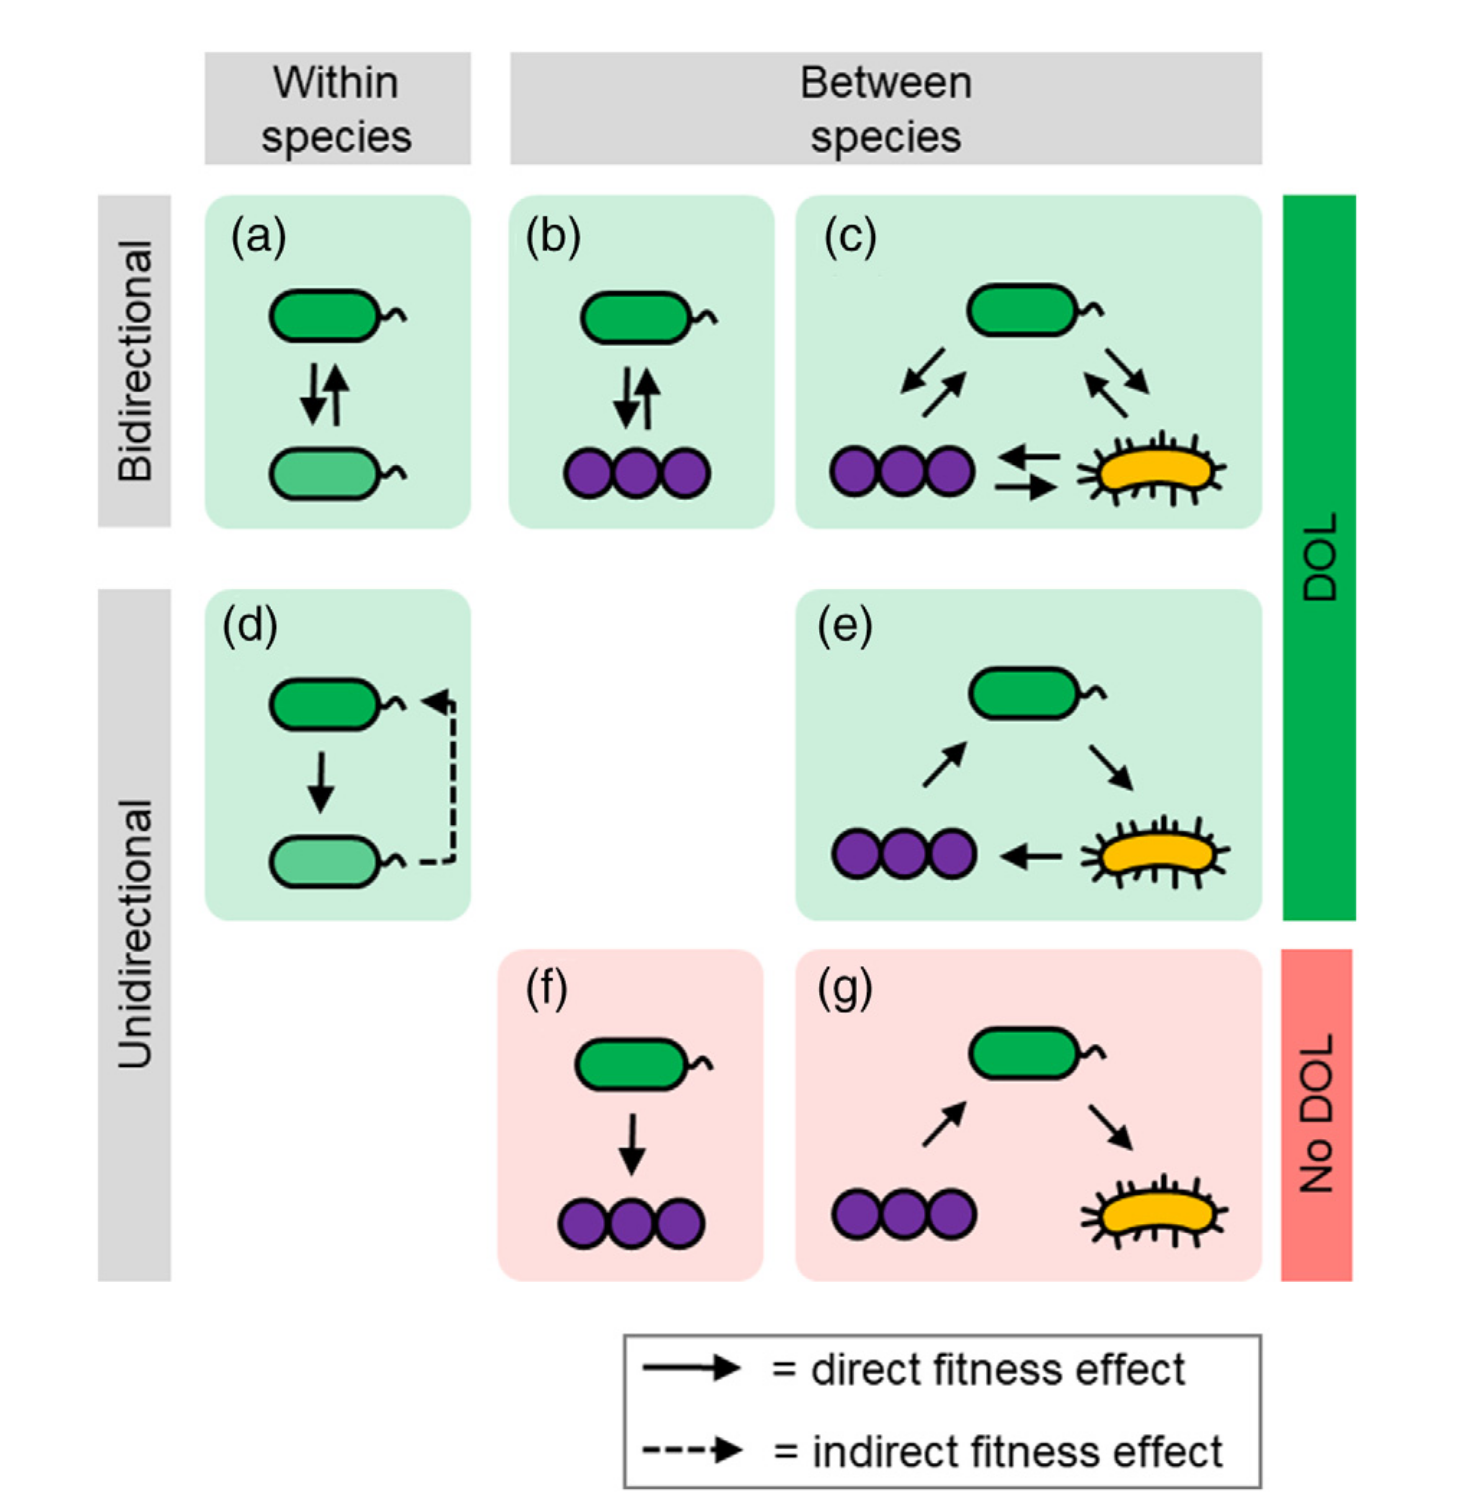
\includegraphics[width=0.6\linewidth,height=\textheight,keepaspectratio]{chapters/../figures/DoL_bacteria.png}

}

\caption{\label{fig-microbial-DoL}Division of Labor in Microbial
Communities (from Giri et al.~2019)}

\end{figure}%

\emph{Classification of pairwise and three-way interactions as DoL.
Interactions can be uni- or bidirectional as well as occur within one or
between two microbial species. Arrows indicate fitness benefits that are
exchanged between interaction partners that can be direct (straight
line) or indirect (dashed line). For an interaction to classify as DoL,
four main criteria need to be fulfilled, which is only the case in
closed (reciprocal) interactions (green), yet not in open (linear)
interactions (red). (a) Mutually beneficial (reciprocal) interaction
within two conspecific genotypes. (b) Mutually beneficial (reciprocal)
interaction within two heterospecific genotypes. (c) Mutually beneficial
(reciprocal) interaction between three different species. (d)
Unidirectional interaction between two members of the same species. (e)
Unidirectional interaction between three members of three different
species. (f) Unidirectional interaction between two members of two
different species. (g) Unidirectional (linear) interaction chain between
members of three different species.}

\section{Division of Labor in Root
Microbiota}\label{division-of-labor-in-root-microbiota}

Interspecific DoL has been well-characterized in various ecosystems,
with numerous examples of cross-feeding and mutualistic interactions
documented in the human gut microbiome and soil
communities\textsuperscript{\citeproc{ref-rafieenia2022}{4}}.

The root microbiota represents a particularly well-studied example of
interspecific DoL. Roots of healthy plants host diverse bacteria that
are collectively referred to as the bacterial root microbiota. Unlike
their multicellular eukaryotic hosts that evolved diverse cell-types to
achieve distinct biological functions and promote a division of labour,
unicellular organisms such as bacteria rely on metabolic exchange(s)
with their surrounding biotic environment to establish and maintain
their ecological niches. Recent
reports\textsuperscript{\citeproc{ref-mataigne2021}{5},\citeproc{ref-mataigne2022}{6}},
indicate that metabolic interdependencies and cross-feeding exchanges
are widespread among taxonomically diverse bacteria and likely drive
microbial co-existence within complex bacterial
communities\textsuperscript{\citeproc{ref-estrela2016}{7},\citeproc{ref-adkins-jablonsky2021}{8}}.

While interspecific DoL has been extensively studied, intraspecific DoL
within clonal/isogenic bacterial populations remains less explored,
despite its potential importance for understanding population-level
adaptation and functional diversity. The traditional view of biological
populations assumed that all individuals within a clonal population
behave identically. However, evidence has accumulated over decades
showing that even genetically identical organisms can exhibit functional
heterogeneity, leading to population-level benefits through task
specialization\textsuperscript{\citeproc{ref-giri2019}{2}}
\textsuperscript{\citeproc{ref-luxf3pez-paguxe1n2025}{9}}.

A major unsolved question is whether populations of genetically
identical bacteria can minimise energetically costly processes by each
executing different metabolic tasks at the intra-population level. Here,
we hypothesise that metabolic cooperation within bacterial populations
plays a key role in modulating population dynamics, competitiveness, and
persistence at the root--soil interface. This hypothesis builds on the
idea that bacteria are subject to stochastic, noisy gene
expression\textsuperscript{\citeproc{ref-raj2008}{10}--\citeproc{ref-chowdhury2021}{12}}.
In such systems, not all individuals respond identically to
environmental cues, leading to phenotypic heterogeneity. This
noise-driven diversity can be beneficial at the population level. The
theory of Noise-Averaging Cooperation
(NAC)\textsuperscript{\citeproc{ref-lopez2022}{13}} further proposes
that metabolic noise---exacerbated by the small size of bacteria---can
constrain individual growth, but can be mitigated through metabolite
sharing among related cells. This ``leaky function'', forming a
``metabolic marketplace'', allows populations to buffer stochastic
fluctuations and improve collective fitness. In this context,
cross-feeding interactions may emerge as a result of gene expression
variability and/or the selection of advantageous mutations, fostering
metabolic interdependencies within the population (see
Figure~\ref{fig-intraspecific-DoL}).

Finally, environmental regulation also shapes this process:
microenvironmental cues and spatial heterogeneity can induce
context-dependent gene expression
patterns\textsuperscript{\citeproc{ref-luxf3pez-paguxe1n2025}{9},\citeproc{ref-korshoj2024}{14}},
which, if consistently beneficial, may become genetically encoded over
evolutionary time. Altogether, these mechanisms point toward an
intra-population division of labour emerging from the interplay between
gene expression noise, environmental signals, and evolutionary
selection.

\begin{figure}

\centering{

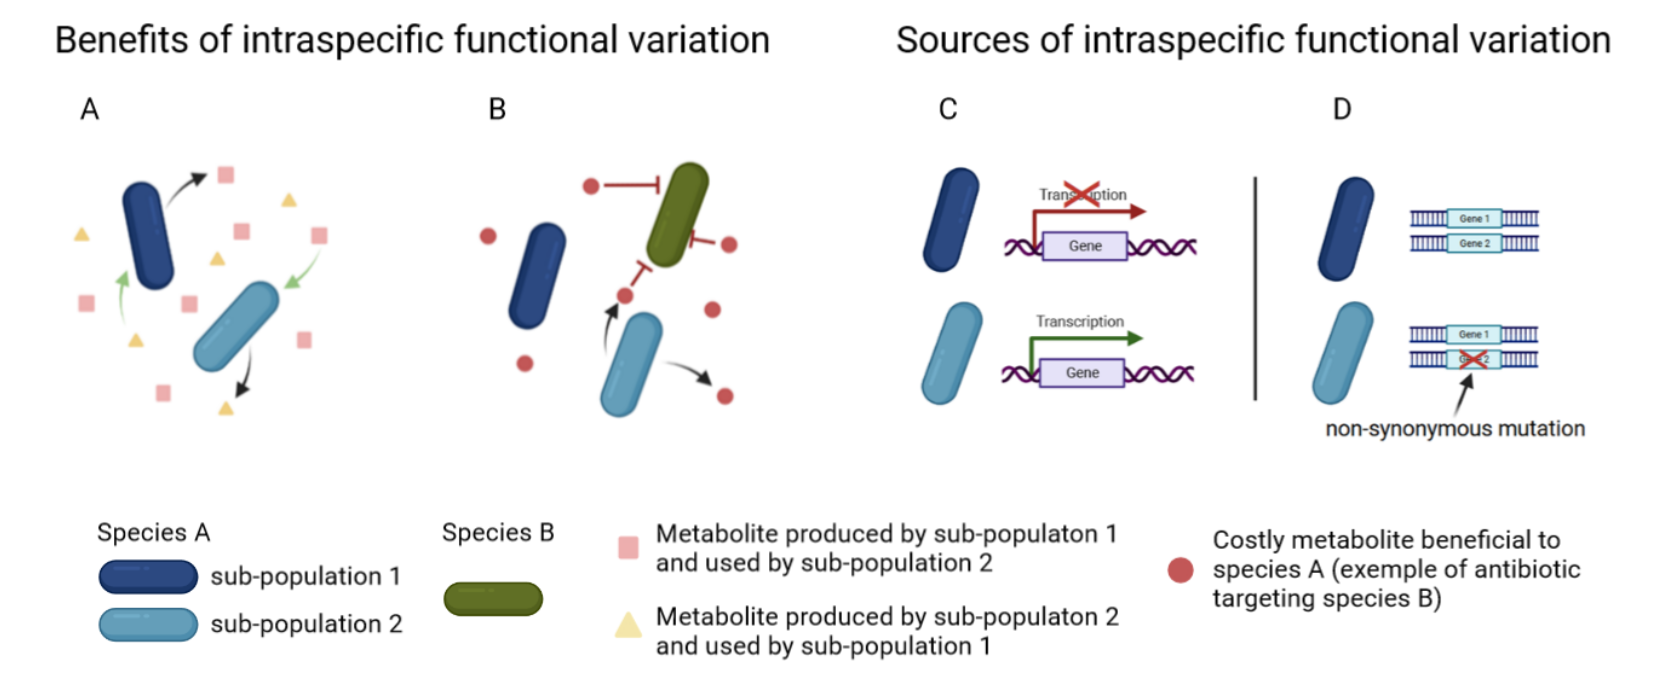
\includegraphics[width=0.9\linewidth,height=\textheight,keepaspectratio]{chapters/../figures/intraspecific_DoL.png}

}

\caption{\label{fig-intraspecific-DoL}Examples of benefits and sources
of intraspecific division of labour between intra-populations based on
metabolic complementation and costly ``common good'' metabolite
production.}

\end{figure}%

\emph{From the left to the right, co-metabolism within an isogenic
bacterial population (A) and production of antimicrobials targeting
other bacteria (B) can be considered as division of labour in a
population. These mechanisms of division of labour can be based on
differential transcription between bacteria (C) within a population
and/or genetic variations between intra-populations (D).}

\section{\texorpdfstring{\emph{PsR401}: A Model System for Studying
Intraspecific
DoL}{PsR401: A Model System for Studying Intraspecific DoL}}\label{psr401-a-model-system-for-studying-intraspecific-dol}

To investigate these theoretical frameworks of intraspecific DoL, we
require a well-characterized bacterial model system that exhibits the
complex metabolic interactions described above. Successful establishment
of bacteria at roots is driven by multiple independent biological
processes involved in both host-microbe (i.e., signal recognition,
chemotaxis, surface attachment, biofilm formation, virulence
factors)\textsuperscript{\citeproc{ref-luxf3pez-paguxe1n2025}{9}} and
microbe-microbe interactions (i.e., production of antimicrobials or
public goods)\textsuperscript{\citeproc{ref-knights2021}{15}}.
Therefore, we postulate that the simultaneous activation of these
diverse processes is costly and that cooperation between genetically
identical strains is key for promoting bacterial pervasiveness at roots.
Consistent with this hypothesis, it was recently demonstrated that the
robust root coloniser \emph{Pseudomonas brassicacearum R401} (hereafter
referred to as \emph{PsR401}) deploys multiple independent strategies
that co-function to promote colonisation and persistence at
roots\textsuperscript{\citeproc{ref-getzke2023}{16}}. Unlike many
pathogenic bacteria, \emph{PsR401} lacks genes for a type III secretion
system (T3SS) and does not overgrow or suppress plant immune
responses\textsuperscript{\citeproc{ref-jian2024}{17},\citeproc{ref-dodds2024}{18}}.
This opportunistic
pathogen\textsuperscript{\citeproc{ref-getzke2024}{19}} of the plant
model \emph{Arabidopsis thaliana} acts as a potent antagonist that
relies on the combined action of three distinct exometabolites to
suppress competitors and promote root colonization.

First, this Gram-negative bacterium produces a phytotoxin called
Brassicapeptin\textsuperscript{\citeproc{ref-getzke2024}{19},\citeproc{ref-chesneau2025}{20}},
which promotes both pathogenicity and root colonization in
mono-association experiments with Arabidopsis thaliana. Second, PsR401
synthesizes 2,4-diacetylphloroglucinol
(DAPG)\textsuperscript{\citeproc{ref-getzke2023}{16}}, an antimicrobial
compound that directly inhibits competing microbes. Third, it produces
pyoverdine\textsuperscript{\citeproc{ref-getzke2023}{16}}, a siderophore
that chelates iron from the environment---an essential but scarce
micronutrient in the
rhizosphere\textsuperscript{\citeproc{ref-cao2024}{21}}.

Iron availability plays a central role in microbial interactions at the
root--soil interface. It also delineates iron as a major micronutrient
modulating strain competitiveness and proliferation at
roots\textsuperscript{\citeproc{ref-gu2020}{22},\citeproc{ref-harbort2020}{23}}.
In iron-limited environments, siderophore-mediated iron scavenging
confers a strong competitive advantage by depriving rival microbes of
access to this vital resource. Resource competition, especially for
iron, thus represents a key mechanism of indirect microbial antagonism.
Beyond simply acquiring nutrients, microbes may also sequester them,
preventing uptake by others and modulating community composition and
function\textsuperscript{\citeproc{ref-mesny2023}{24}}.

\begin{tcolorbox}[enhanced jigsaw, arc=.35mm, colbacktitle=quarto-callout-tip-color!10!white, rightrule=.15mm, title=\textcolor{quarto-callout-tip-color}{\faLightbulb}\hspace{0.5em}{Biological Hypothesis}, coltitle=black, bottomrule=.15mm, left=2mm, opacityback=0, colback=white, toprule=.15mm, toptitle=1mm, titlerule=0mm, breakable, bottomtitle=1mm, opacitybacktitle=0.6, colframe=quarto-callout-tip-color-frame, leftrule=.75mm]

Given that iron functions as a public good whose availability becomes
rate-limiting in the root compartment and that production of the
above-mentioned processes are all modulated by iron
availability,\textsuperscript{\citeproc{ref-lim2012}{25}} we propose
that division of labour (DoL) among genetically identical PsR401 cells
may be reinforced under iron-limiting conditions, such as those found in
the root habitat. In such scenarios, phenotypic heterogeneity---whether
driven by gene expression noise or environmentally induced
regulation---could lead to subpopulations specialising in complementary
tasks, such as toxin production, antimicrobial defense, or
siderophore-mediated iron acquisition, thereby enhancing
population-level fitness.

\end{tcolorbox}

\section{Leveraging Single-Cell Transcriptomics to Study
DoL}\label{leveraging-single-cell-transcriptomics-to-study-dol}

To test our biological hypothesis regarding intraspecific DoL in
\emph{PsR401}, we need to examine transcriptional heterogeneity at the
single-cell level. Traditionally, studies of bacterial gene expression
have relied on bulk RNA sequencing methods, which provide an average
view of the transcriptome across a
population.\textsuperscript{\citeproc{ref-nishimura2025}{26}} However,
these approaches mask the underlying cell-to-cell variability that is
critical for understanding complex bacterial behaviors and adaptations.
The advent of single-cell RNA sequencing (scRNA-seq) and now multi-omics
technologies has provided unprecedented insights into cellular
heterogeneity across various biological
systems\textsuperscript{\citeproc{ref-vandereyken2023}{27}--\citeproc{ref-nobori}{29}}.
Although eukaryotic cells have benefited from scRNA-seq technology since
2009, prokaryotic systems have faced significant implementation delays
owing to distinct technical obstacles. These challenges include low RNA
content in individual cells, the absence of poly-A tails on bacterial
mRNAs, and diverse cell wall
structures.\textsuperscript{\citeproc{ref-nishimura2025}{26}} These
factors necessitate the development of specialized techniques for
efficient cell lysis, RNA extraction, and mRNA enrichment in bacterial
systems. Despite these challenges, recent years have seen significant
progress in developing and refining bacterial scRNA-seq
methods\textsuperscript{\citeproc{ref-nishimura2025}{26},\citeproc{ref-sarfatis2025}{30}}.
These methodological improvements have created novel opportunities to
explore bacterial physiology, stress responses, and population dynamics
at single-cell resolution.

\section{Research Objectives and
Approach}\label{research-objectives-and-approach}

\subsection{Our Focus: microSPLiT
Technology}\label{our-focus-microsplit-technology}

To address our biological hypothesis regarding intraspecific DoL in
\emph{PsR401}, we will leverage the microSPLiT (microbial Split-Pool
Ligation Transcriptomics)
technology\textsuperscript{\citeproc{ref-kuchina2021}{31},\citeproc{ref-gaisser2024}{32}}.
This cutting-edge bacterial scRNA-seq method enables high-throughput
profiling of individual bacterial cells, providing the resolution
necessary to detect transcriptional heterogeneity within clonal
populations. By analyzing \emph{PsR401} cells under contrasting nutrient
conditions---particularly iron-limited versus iron-replete
environments---we hope to identify potential subpopulations that
specialize in different metabolic tasks (see
Figure~\ref{fig-hypothesis-iron}).

\begin{figure}

\centering{

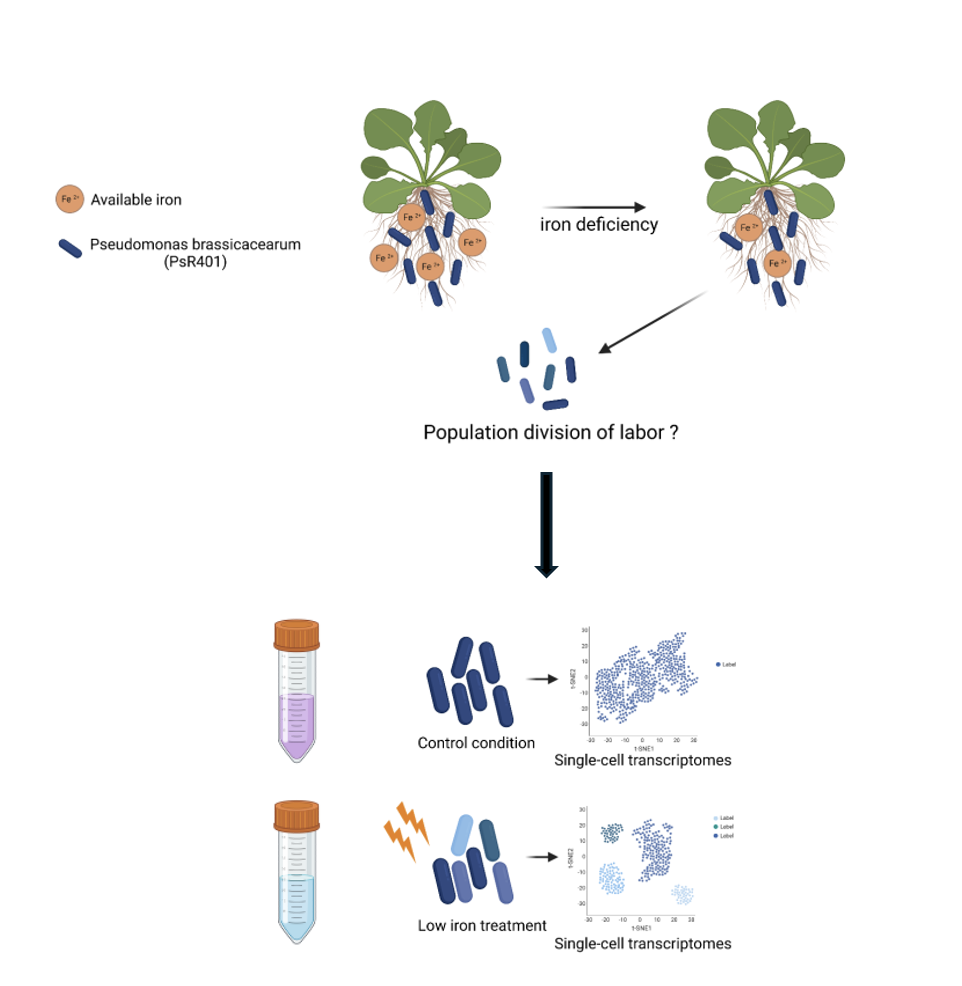
\includegraphics[width=0.8\linewidth,height=\textheight,keepaspectratio]{chapters/../figures/DoL_hypothesis.png}

}

\caption{\label{fig-hypothesis-iron}Hypothesis of DoL in \emph{PsR401}
under iron-limiting conditions}

\end{figure}%

\emph{Testing the division of labor hypothesis in PsR401 under two
contrasting conditions: iron-limited and iron-replete environments.
Single-cell RNA sequencing (scRNA-seq) with microSPLiT will enable
detection of transcriptional heterogeneity within the population,
revealing whether this specialization is driven by gene expression noise
or environmentally induced metabolic specialization in both
environmental conditions.}

\subsection{Internship Goals and Expected
Outcomes}\label{internship-goals-and-expected-outcomes}

Building upon the theoretical framework of intraspecific division of
labor and the biological characteristics of \emph{PsR401}, this
internship aims to leverage cutting-edge single-cell transcriptomics to
investigate metabolic cooperation within clonal bacterial populations.
The primary goal is to validate the microSPLiT technology for bacterial
systems while testing our hypothesis that iron limitation promotes
functional specialization among genetically identical cells.

Through systematic analysis of transcriptional heterogeneity under
contrasting iron conditions in culture medium, we expect to uncover
whether \emph{PsR401} populations exhibit distinct subpopulations with
specialized metabolic functions or whether cooperation emerges through
noisy gene expression regulation across the population. By examining
temporal dynamics of gene expression patterns, we will gain insights
into how these cooperative behaviors evolve and stabilize over time.
This investigation will provide critical insights into the mechanisms
underlying population-level adaptation and resilience, particularly in
the context of fluctuating iron availability.

The expected outcomes of this research extend beyond understanding
\emph{PsR401} biology. By establishing robust methodologies for
bacterial single-cell transcriptomics, this work will contribute to the
broader field of microbial population dynamics.

Ultimately, this project will advance our understanding of how
phenotypic diversity among clonal bacterial populations facilitates
ecological success and resilience during root colonization, while
establishing methodological foundations for future studies of bacterial
population dynamics at single-cell resolution.

\bookmarksetup{startatroot}

\chapter{Materials and Methods}\label{sec-materials-and-methods}

\section{Bacterial culture}\label{bacterial-culture}

\begin{figure}

\centering{

\includegraphics[width=4in,height=3in]{chapters/02-Materials-and-methods_files/figure-latex/mermaid-figure-1.png}

}

\caption{\label{fig-experimental-design}Experimental design for
bacterial culture}

\end{figure}%

\emph{The workflow illustrates the progression from initial culture of
P. brassicacearum R401 on petri dishes to liquid culture in two
different media: M9 (low glucose and iron) and M9F (high glucose and
iron). Each medium condition was replicated three times (Rep A, B, C)
and growth was monitored at three timepoints (T1, T2, T3) by optical
density measurements. This design resulted in 18 total experimental
conditions (2 media × 3 biological replicates × 3 timepoints) for
subsequent single-cell RNA-seq analysis.}

An isogenic\footnote{An isogenic population refers to a group of
  organisms that are genetically identical, derived from a single
  ancestral cell or clone.} population of \emph{P. brassicacearum} R401
was initially cultured on petri dishes and then transferred to different
liquid media to investigate the effects of nutrient availability on
bacterial growth and gene expression
(Figure~\ref{fig-experimental-design}).

Two distinct culture conditions were applied to the bacteria: M9 medium
containing low glucose and low iron concentrations, and M9F medium
containing high glucose and high iron concentrations (see
Table~\ref{tbl-media} for detailed concentrations). Each condition was
replicated three times to ensure statistical robustness of the
experimental results. The bacterial growth was monitored by measuring
optical density (OD) at regular intervals. The growth curves obtained
from these measurements are presented (Figure~\ref{fig-growth-curves})
and (Table~\ref{tbl-growth-curves}). This experimental design resulted
in a total of 18 conditions: 2 media types × 3 biological replicates × 3
time points, providing comprehensive coverage of the growth dynamics
under different nutrient conditions.

\begin{figure}

\centering{

\pandocbounded{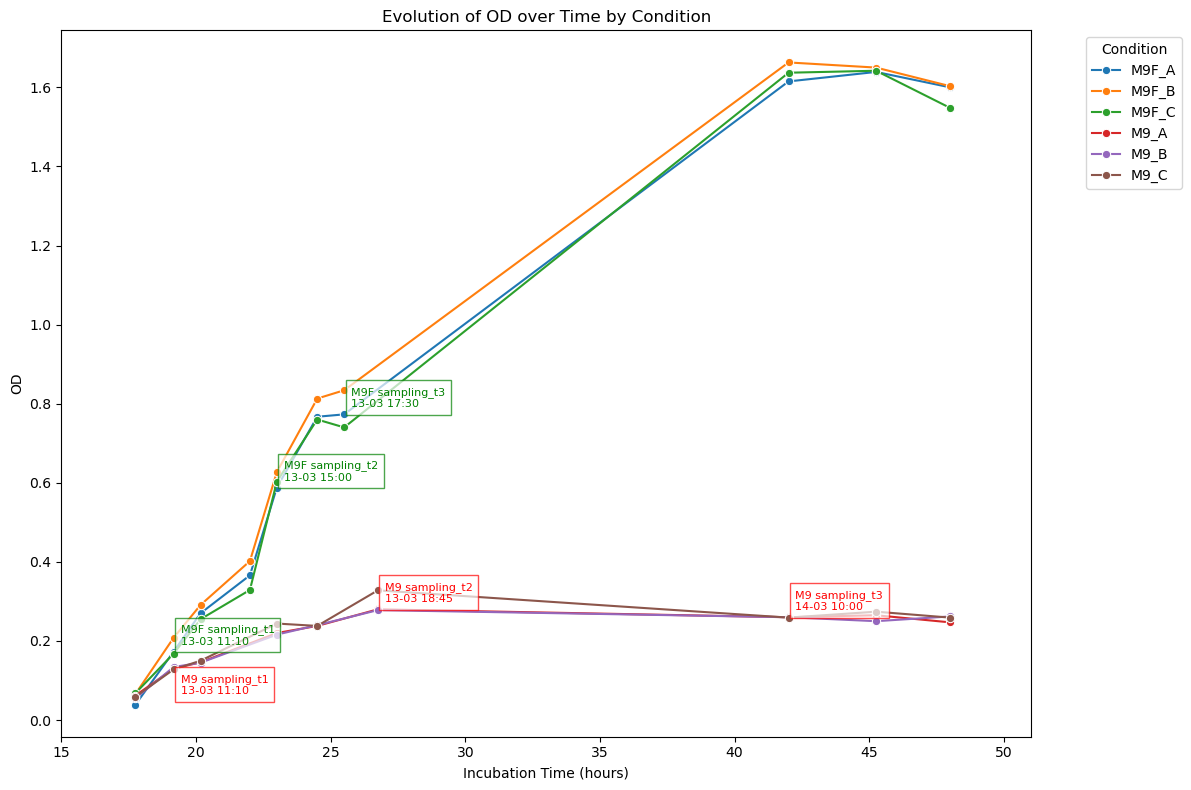
\includegraphics[keepaspectratio]{chapters/../figures/growth_curves_all.png}}

}

\caption{\label{fig-growth-curves}Bacterial growth dynamics of \emph{P.
brassicacearum} R401 populations measured by optical density (OD600)
cultured under two different nutrient conditions: M9 (low glucose/iron)
and M9F (high glucose/iron).}

\end{figure}%

\emph{Measurements were taken at three timepoints (T1, T2, T3) for three
biological replicates (Rep A, B, C).}

The growth curves reveal distinct patterns between the two culture
conditions. Bacteria grown in M9F medium (high glucose and iron)
exhibited significantly higher growth rates and reached higher optical
densities (OD 0.17-0.21 at T1, 0.59-0.63 at T2, 0.74-0.83 at T3)
compared to M9 medium (low glucose and iron) which showed limited growth
(OD 0.13 at T1, 0.28-0.33 at T2, 0.26 at T3). While M9F cultures showed
continued growth from T2 to T3, the growth rate slowed down during this
period, indicating the beginning of transition towards stationary phase.
The M9 cultures appeared to reach a growth plateau by T3, while M9F
cultures maintained higher densities despite the growth deceleration,
suggesting nutrient limitation in the M9 condition. Biological
replicates showed excellent reproducibility validating the experimental
design.

Cells were collected at each timepoint (T1, T2, T3) from all biological
replicates for subsequent single-cell RNA-seq analysis using the
Microbial split-pool ligation transcriptomics (microSPLiT)
protocol\textsuperscript{\citeproc{ref-kuchina2021}{31},\citeproc{ref-gaisser2024}{32}}.

\section{microSPLiT protocol}\label{microsplit-protocol}

MicroSPLiT\textsuperscript{\citeproc{ref-kuchina2021}{31},\citeproc{ref-gaisser2024}{32}}
is a high-throughput single-cell RNA sequencing method for bacteria,
capable of profiling transcriptional states in hundreds of thousands of
cells per experiment without the need for specialized
equipment\textsuperscript{\citeproc{ref-nishimura2025}{26},\citeproc{ref-gaisser2024}{32}}.
Unlike other single-cell RNA-seq approaches that require physical
isolation of individual cells (e.g., plate-based or droplet-based
methods), microSPLiT uses a split-pool barcoding strategy to uniquely
label transcripts within each cell. (see
Figure~\ref{fig-nishimura_review} for an overview of single-cell RNA-seq
methods in bacteria)

\begin{tcolorbox}[enhanced jigsaw, arc=.35mm, colbacktitle=quarto-callout-tip-color!10!white, rightrule=.15mm, title=\textcolor{quarto-callout-tip-color}{\faLightbulb}\hspace{0.5em}{Information}, coltitle=black, bottomrule=.15mm, left=2mm, opacityback=0, colback=white, toprule=.15mm, toptitle=1mm, titlerule=0mm, breakable, bottomtitle=1mm, opacitybacktitle=0.6, colframe=quarto-callout-tip-color-frame, leftrule=.75mm]

The microSPLiT strategy will not be described in detail here; for more
information, see Gaisser
protocol.\textsuperscript{\citeproc{ref-gaisser2024}{32}}. Only the key
steps necessary for a general understanding of the method are presented
below.

\end{tcolorbox}

\begin{figure}

\centering{

\pandocbounded{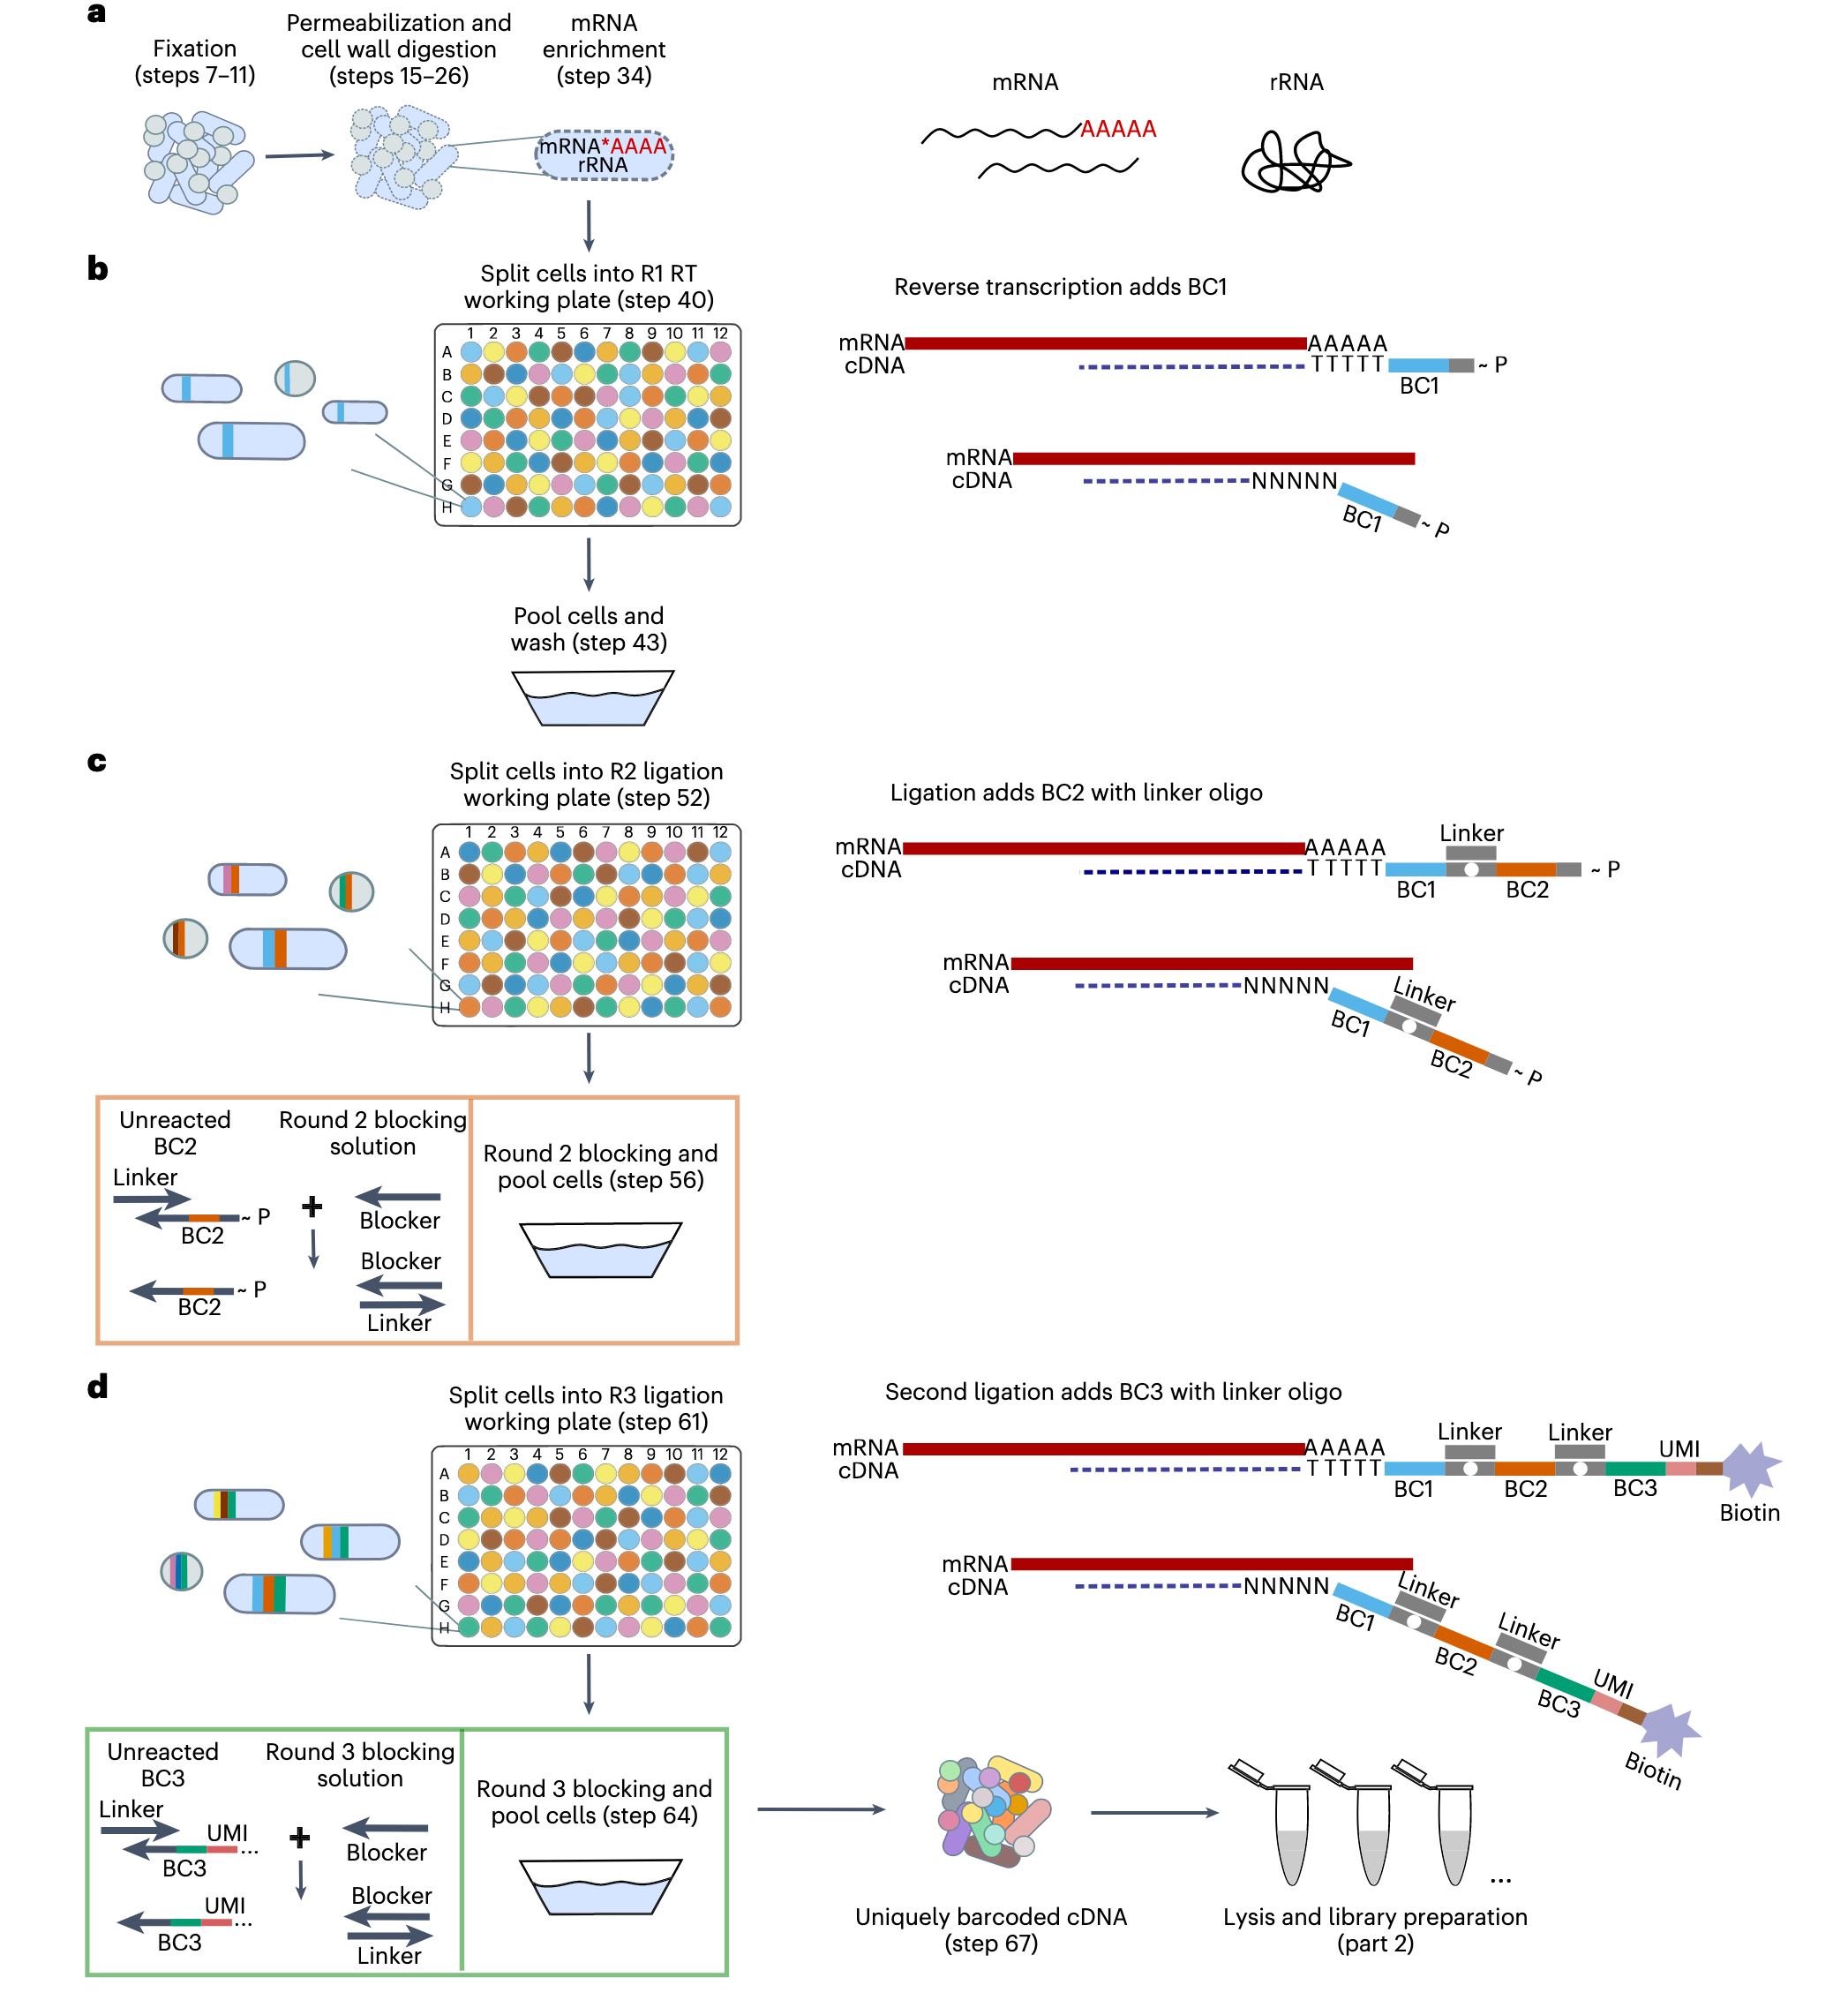
\includegraphics[keepaspectratio]{chapters/../figures/protocol.png}}

}

\caption{\label{fig-protocol}MicroSPLiT in-cell cDNA barcoding scheme.}

\end{figure}%

\emph{a, Bacterial cells are fixed overnight and permeabilized before
the mRNA is preferentially polyadenylated. After mRNA enrichment, cells
may contain both polyadenylated and non-polyadenylated mRNA. b, Cells
are distributed into the first barcoding plate, and the mRNA is reverse
transcribed by using a mixture of poly-dT and random hexamer primers
carrying a barcode (barcode 1, BC1) and a 5' phosphate for future
ligation at their 5' end. After the barcoding reaction, cells are pooled
together and split again into the second barcoded plate. c, Ligation
adds a 5' phosphorylated barcode 2 (BC2) to BC1 with a linker strand. A
blocking solution is then added to each of the wells of the second
plate, preventing any unreacted BC2 from future ligation. Cells are
pooled and split into the third and final barcoded plate. d, A second
ligation step adds barcode 3 (BC3) with another linker strand. BC3 also
contains a 5' biotin, a primer binding site and a unique molecular
identifier (UMI). A blocking solution for the R3 linker is added to each
of the wells in the plate before the final pooling of cells. This
results in uniquely barcoded cells that can be distributed in aliquots
into sub-libraries and stored until future use or used immediately for
library preparation. (R1, round 1; R2, round 2; R3, round
3).\textsuperscript{\citeproc{ref-gaisser2024}{32}}}

\subsection{Fixation and
permeabilization}\label{fixation-and-permeabilization}

The first step is fixation of the bacterial suspension with formaldehyde
Figure~\ref{fig-protocol} immediately after sampling the 18 conditions
Figure~\ref{fig-experimental-design}. This preserves the transcriptomic
state and cross-links RNA to proteins, preventing leakage of each cell's
transcriptome. Next, cells are permeabilized using mild detergent and
lysozyme, allowing enzymes and oligonucleotides to access intracellular
RNA for barcoding.

\begin{tcolorbox}[enhanced jigsaw, arc=.35mm, colbacktitle=quarto-callout-note-color!10!white, rightrule=.15mm, title=\textcolor{quarto-callout-note-color}{\faInfo}\hspace{0.5em}{Note}, coltitle=black, bottomrule=.15mm, left=2mm, opacityback=0, colback=white, toprule=.15mm, toptitle=1mm, titlerule=0mm, breakable, bottomtitle=1mm, opacitybacktitle=0.6, colframe=quarto-callout-note-color-frame, leftrule=.75mm]

Adequate permeabilization is essential for efficient barcoding, but
over-permeabilization can compromise cell integrity. For successful
single-cell resolution, cells must remain intact after permeabilization
to allow multiple split-pool steps and retain cross-linked RNA.
Figure~\ref{fig-protocol}

\end{tcolorbox}

\subsection{mRNA enrichment}\label{mrna-enrichment}

After permeabilization, the transcripts in the fixed and permeabilized
cells undergo in situ polyadenylation with the addition of a poly(A)
polymerase (PAP) and ATP. This step enriches for mRNA in the total
barcoded RNA pool because, under these conditions, PAP preferentially
polyadenylates mRNA as opposed to ribosomique RNA (rRNA)
Figure~\ref{fig-protocol}.

\subsection{Barcoding}\label{barcoding}

\begin{tcolorbox}[enhanced jigsaw, arc=.35mm, colbacktitle=quarto-callout-tip-color!10!white, rightrule=.15mm, title=\textcolor{quarto-callout-tip-color}{\faLightbulb}\hspace{0.5em}{Tip}, coltitle=black, bottomrule=.15mm, left=2mm, opacityback=0, colback=white, toprule=.15mm, toptitle=1mm, titlerule=0mm, breakable, bottomtitle=1mm, opacitybacktitle=0.6, colframe=quarto-callout-tip-color-frame, leftrule=.75mm]

\textbf{The protocol utilizes several rounds of split-pool barcoding
where cells are distributed into 96-well plates, barcoded, pooled, and
redistributed for subsequent rounds, creating unique barcode
combinations that identify individual cells.}

\end{tcolorbox}

\subsubsection{Barcoding round 1 (R1) to identify the condition and the
technical
replicate}\label{barcoding-round-1-r1-to-identify-the-condition-and-the-technical-replicate}

Each of the 18 samples is split into 5 technical replicates for
barcoding, resulting in 90 subsamples. These technical replicates are
then distributed into individual wells of a 96-well plate (6 wells not
used), with each well containing uniquely barcoded primers
Figure~\ref{fig-protocol}. In each well, mRNA is reverse transcribed
into cDNA using a mix of barcoded poly(T) and random hexamer primers.
The primers used in each well contain either a dT15 sequence to capture
polyadenylated mRNA or six random nucleotides to bind any RNA, followed
by a universal sequence for subsequent ligation steps. By assigning each
technical replicate to a specific well, all cells in the same well
receive the same unique barcode during reverse transcription. This
allows each technical replicate and condition to be identified later
based on the first barcode.

\subsubsection{Barcoding rounds 2 (R2) and 3 (R3) for unique cell and
transcript
identification}\label{barcoding-rounds-2-r2-and-3-r3-for-unique-cell-and-transcript-identification}

Cells are then pooled, washed and randomly redistributed into a new
96-well plate (round 2 (R2) ligation working plate) containing a second
set of well-specific barcodes, which are appended to the first barcode
on the cDNA through an in-cell ligation reaction
Figure~\ref{fig-protocol}. Due to the random redistribution of cells,
each well of the second-round plate is likely to contain a mix of cells
with different first-round barcodes, resulting in highly diverse barcode
combinations. The ligation reaction is carried out by the T4 DNA ligase,
which requires double-stranded DNA. Therefore, in the second barcoding
plate, each barcode is first hybridized to a short linker
oligonucleotide whose overhang is complementary to the universal
sequence at the 5' end of the RT barcodes. Figure~\ref{fig-protocol}.

\begin{tcolorbox}[enhanced jigsaw, arc=.35mm, colbacktitle=quarto-callout-note-color!10!white, rightrule=.15mm, title=\textcolor{quarto-callout-note-color}{\faInfo}\hspace{0.5em}{Note}, coltitle=black, bottomrule=.15mm, left=2mm, opacityback=0, colback=white, toprule=.15mm, toptitle=1mm, titlerule=0mm, breakable, bottomtitle=1mm, opacitybacktitle=0.6, colframe=quarto-callout-note-color-frame, leftrule=.75mm]

After the ligation step, some barcodes may remain unreacted in the
solution. To prevent these free barcodes from attaching non-specifically
to DNA from other cells during pooling, a blocker strand is added. This
blocker has a longer complementary region to the linker, allowing it to
displace any unreacted barcodes from the linker and thus ensures that
only correctly ligated barcodes remain attached to the cDNA.
Figure~\ref{fig-protocol}

\end{tcolorbox}

Cells are then pooled again, and a split-ligation-pool cycle is repeated
for the second time. Cells are randomly distributed into a third 96-well
plate (round 3 (R3) ligation working plate), which is loaded with
barcoded oligonucleotides containing the third cell barcode annealed
with a linker, a 10-base Unique Molecular Identifier (UMI), a universal
PCR handle and a 5' biotin\footnote{Biotin is a small vitamin molecule
  that binds with extremely high affinity to streptavidin. This
  biotin-streptavidin interaction is used for the selective capture and
  purification of biotinylated cDNA molecules on streptavidin-coated
  beads during the library preparation process.} molecule. The ligation
reaction is stopped by adding a second blocker strand and EDTA.

\begin{tcolorbox}[enhanced jigsaw, arc=.35mm, colbacktitle=quarto-callout-warning-color!10!white, rightrule=.15mm, title=\textcolor{quarto-callout-warning-color}{\faExclamationTriangle}\hspace{0.5em}{Warning}, coltitle=black, bottomrule=.15mm, left=2mm, opacityback=0, colback=white, toprule=.15mm, toptitle=1mm, titlerule=0mm, breakable, bottomtitle=1mm, opacitybacktitle=0.6, colframe=quarto-callout-warning-color-frame, leftrule=.75mm]

In our experiment, only 95 out of the 96 wells of the R3 plate are used
to minimize potential bias in cell distribution. This setup allows for
90 × 96 × 95 = \textbf{820,800 possible barcode combinations}, enabling
the identification of up to 820,800 individual cells.

\end{tcolorbox}

\subsection{Sub-library and sequencing
preparation}\label{sub-library-and-sequencing-preparation}

The pooled cells are washed, counted, and divided into multiple
sub-libraries. Only sub-libraries containing approximately 3,000 cells
were selected for sequencing, in order to maximize sequencing depth per
cell and minimize barcode collision rates which is the probability that
two cells receive the same barcode combination.

After lysis and cDNA purification on streptavidin beads
(Figure~\ref{fig-protocol-p2}), a second reverse transcription is
performed to improve cDNA yield, during which a template switch oligo
(TSO) is added to introduce a 3' adapter. The resulting cDNA is then
amplified by PCR. Following amplification, a size selection step removes
short byproducts such as adapter or barcode dimers, ensuring that only
high-quality cDNA fragments are retained for sequencing.

To optimize sequencing depth, the final library was split into four
sub-libraries, each receiving a distinct index during adapter ligation:
BC\_0076 (CAGATC), BC\_0077 (ACTTGA), BC\_0078 (TAGCTT), and BC\_0079
(GGCTAC). These indexes were used solely to improve sequencing quality
and balance on the NovaSeq platform, without introducing any
experimental or technical variation between sub-libraries.

\subsection{Sequencing and demultiplexing
sub-libraries}\label{sequencing-and-demultiplexing-sub-libraries}

Sequencing was performed on a NovaSeq\textsuperscript{TM} X plus
instrument at GenoBIRD platform in paired-end mode. The library pool was
loaded onto all lanes of the flowcell at a final concentration of 200 pM
with 20\% PhiX\footnote{PhiX is a control library containing a known
  viral genome sequence that is spiked into sequencing runs to monitor
  sequencing quality, calibrate base calling, and provide a reference
  for quality control metrics. It helps ensure accurate sequencing
  performance and data quality assessment.}. The sequencing program
consisted of 241 cycles for Read 1, 6 cycles for Index i7 and 91 cycles
for Read 2. The sequencing facility performed demultiplexing of
sub-libraries, resulting in eight FASTQ files (R1 and R2 for each
index). R1 files contain the cDNA sequences, while R2 files contain the
cell barcodes (from the three split-pool rounds) and unique molecular
identifiers (UMIs).

\begin{itemize}
\tightlist
\item
  For each index, two paired-end FASTQ files were generated :

  \begin{itemize}
  \tightlist
  \item
    \textbf{R1} contains the cDNA sequence of interest (transcriptome).
  \item
    \textbf{R2} contains the cell barcodes and unique molecular
    identifiers (UMIs).
  \end{itemize}
\end{itemize}

\section{Pipeline for microSPLiT data
processing}\label{pipeline-for-microsplit-data-processing}

\begin{figure}

\centering{

\pandocbounded{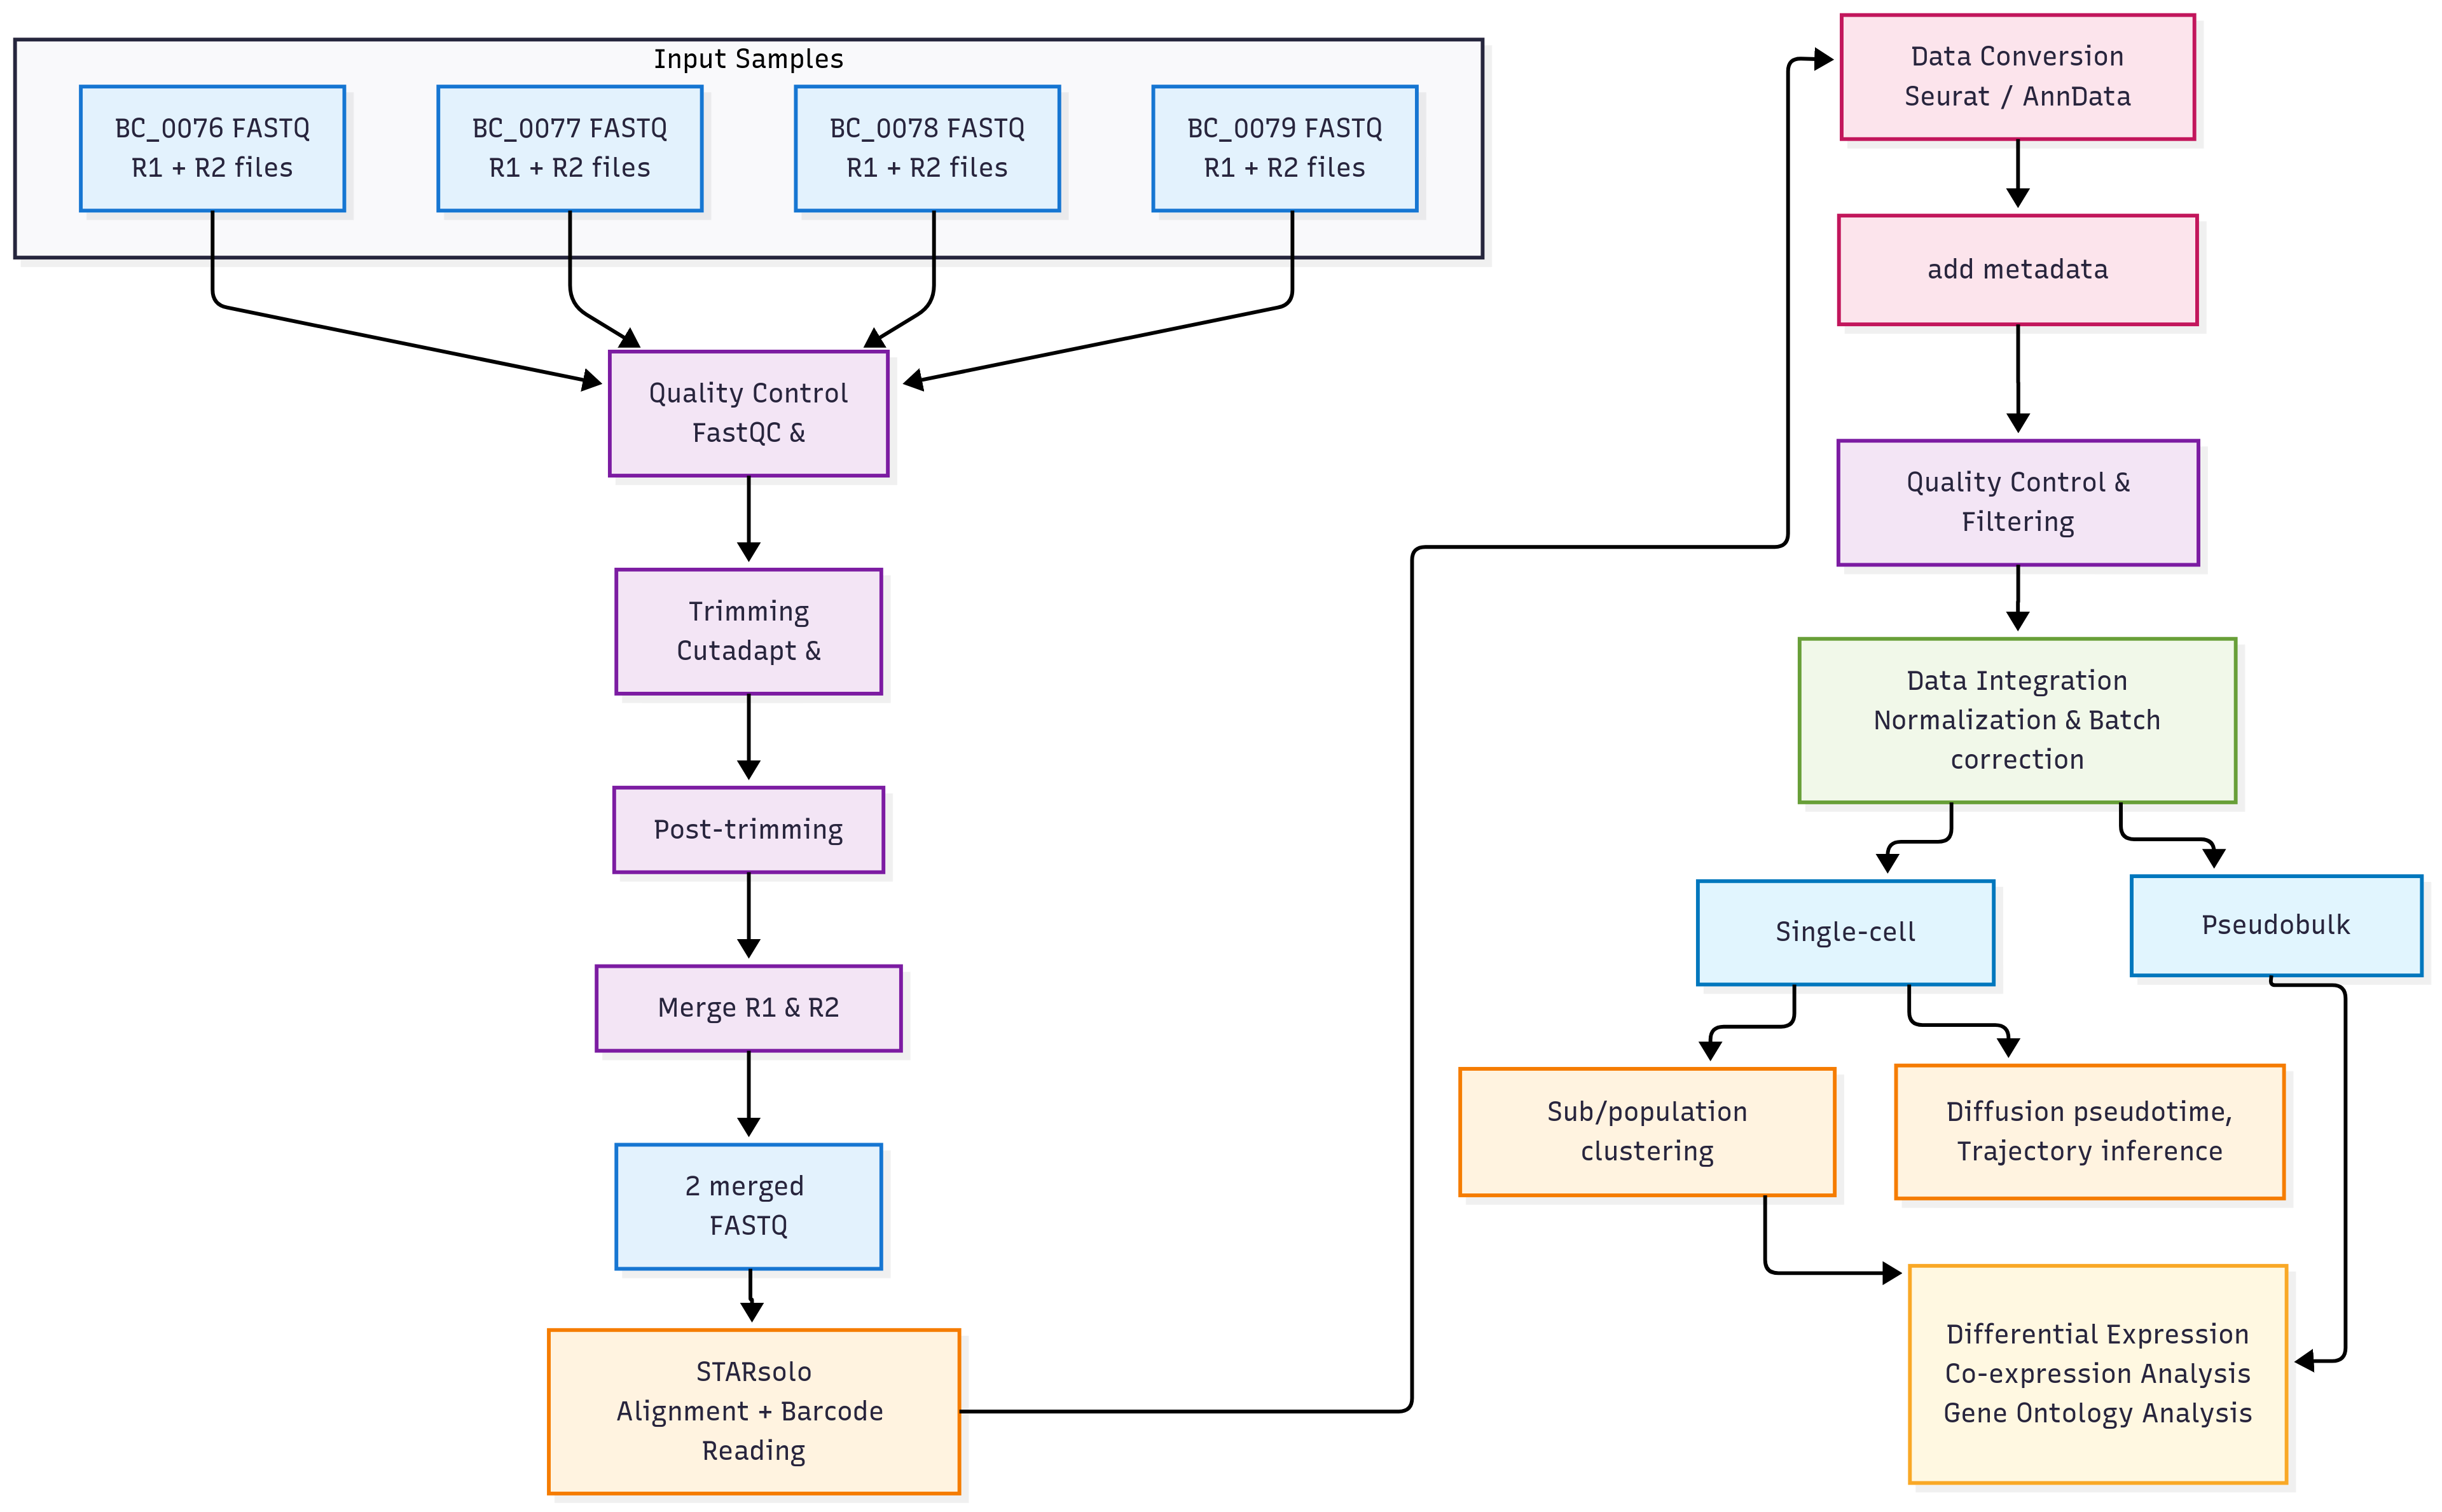
\includegraphics[keepaspectratio]{chapters/../figures/pipeline.png}}

}

\caption{\label{fig-pipeline}Comprehensive pipeline for microSPLiT
single-cell RNA-seq data processing.}

\end{figure}%

\emph{The workflow encompasses the complete analytical process from raw
sequencing data to biological interpretation, including quality control
and preprocessing of FASTQ files, alignment and quantification using
STARsolo, data structuring with metadata assignment, quality filtering
and integration, single-cell and pseudobulk analysis approaches,
population characterization through clustering and trajectory inference,
and downstream expression analysis including differential expression,
co-expression networks, and gene ontology enrichment.
Figure~\ref{fig-pipeline}}

\subsection{Preprocessing of the sequencing
data}\label{preprocessing-of-the-sequencing-data}

All quality control, trimming, alignment, barcode reading and generation
of cell-gene count matrix steps were performed on the GenOuest
high-performance computing cluster using SLURM job scripts and
parallelization to ensure efficient and reproducible analysis of
large-scale sequencing data.

\subsubsection{Quality control and
trimming}\label{quality-control-and-trimming}

Read quality was initially assessed for all four libraries (R1 and R2)
using FastQC\textsuperscript{\citeproc{ref-babraham}{33}} and
MultiQC\textsuperscript{\citeproc{ref-ewels2016}{34}}. Trimming was then
performed with Cutadapt\textsuperscript{\citeproc{ref-martin2011}{35}}
and Fastp\textsuperscript{\citeproc{ref-chen2018}{36}} to clean the
sequencing data. For R2 files, trimming focused on filtering for valid
barcodes. For R1 files, trimming removed various artifacts:
template-switching oligo (TSO) sequences at the 5' end, adapter
sequences, and 3' artifacts including polyG stretches (NovaSeq-specific
artifacts) and potential R1 complement sequences when cDNA was short.
Only reads with a minimum length of 25 bp were kept. The detailed
trimming pipeline is described in Appendix Section
Section~\ref{sec-appendix-trimming-steps}. After trimming, read quality
was reassessed with FastQC\textsuperscript{\citeproc{ref-babraham}{33}}
and MultiQC\textsuperscript{\citeproc{ref-chen2018}{36}}, and results
were merged into unique files (R1 and R2).

\subsubsection{Quality control after
trimming}\label{quality-control-after-trimming}

After trimming, a quality control step was performed to ensure that the
remaining reads were of high quality and suitable for downstream
analysis. This step involved checking the distribution of read lengths,
GC content, and other relevant metrics.

\subsubsection{Merge files}\label{merge-files}

After quality control, the files from all four libraries (R1 and R2 for
each index) were merged into a single file for each index. This step
ensured that all cells from all conditions and technical replicates were
included in the analysis.

\subsubsection{Alignment, barcode reading and generation of cell-gene
count
matrix}\label{alignment-barcode-reading-and-generation-of-cell-gene-count-matrix}

The alignment and quantification pipeline was implemented using
STARsolo\textsuperscript{\citeproc{ref-dobin2013}{37},\citeproc{ref-kaminow}{38}},
an extension of the STAR aligner specifically designed for single-cell
RNA-seq data. STARsolo was chosen based on benchmarking studies showing
it offers the best combination of speed and reproducibility for
SPLiT-seq / microSPLiT data
analysis\textsuperscript{\citeproc{ref-kuijpers2024}{39}}. The
implementation followed the recommendations outlined in Gaisser et
al\textsuperscript{\citeproc{ref-gaisser2024}{32}} for optimal
microSPLiT data processing. Complete pipeline scripts and parameters are
detailed in Appendix Section Section~\ref{sec-appendix-starsolo}.

\textbf{Reference genome and annotation.} The reference genome of
\emph{Pseudomonas brassicacearum} R401:
\href{https://www.ncbi.nlm.nih.gov/datasets/genome/GCA_030064105.1/}{ASM3006410v1
(GCA\_030064105.1)} and its
\href{https://www.ncbi.nlm.nih.gov/datasets/gene/GCA_030064105.1/}{annotation}
were downloaded from GenBank. The GFF3 annotation file was converted to
GTF format using gffread
(Cufflinks\textsuperscript{\citeproc{ref-trapnell2010}{40}} package) for
compatibility with STARsolo.

\textbf{Correcting GTF file for compatibility with STAR.} The conversion
was verified to ensure all required fields were present, particularly
confirming that genes were labeled as `exon' features rather than `CDS'
descriptors, and that chromosome names matched between reference
sequence and annotation files. This correction was performed to ensure
proper compatibility with STARsolo.

\textbf{Alignment parameters.} The pipeline used optimized parameters
for microSPLiT data: minimum 50 matching bases for valid alignment and 1
mismatch tolerance for both barcode and UMI matching. The complex
barcode structure (R2) was configured with positions 0\_10\_0\_17,
0\_48\_0\_55, and 0\_78\_0\_85 for the three barcoding rounds, and UMI
position 0\_0\_0\_9.

\textbf{Output matrices.} STARsolo generated count matrices using
\texttt{GeneFull} feature counting and \texttt{UniqueAndMult-Uniform}
mapping strategy (distributes multi-mapped reads uniformly). Although
bacteria lack introns, \texttt{GeneFull} was chosen to include reads
that may map to intergenic regions or incompletely annotated gene
boundaries, which is common in bacterial genomes. The
\texttt{UniqueAndMult-Uniform} strategy is particularly important for
bacterial genomes due to the presence of paralogous genes, repetitive
sequences, and operon structures that can result in reads mapping to
multiple genomic locations. Raw data matrices (unfiltered barcodes) were
used for downstream
analysis\textsuperscript{\citeproc{ref-gaisser2024}{32}}, with cell
filtering applied later in the processing pipeline.

\textbf{Quality control and output files.} After STARsolo analysis,
quality control was performed using the Log.final.out and summary.csv
files. The main output files for downstream analysis included
barcode.tsv (cell identifiers), features.tsv (gene identifiers), and
UniqueAndMult-Uniform.mtx (count matrix).

\subsection{Single-cell data
processing}\label{single-cell-data-processing}

All downstream analyses were performed locally using a reproducible
development container environment
(Docker\textsuperscript{\citeproc{ref-merkel2014}{41}} and
\href{https://rocker-project.org/images/devcontainer/features.html}{Rocker
Project}) with Visual Studio Code dev containers to ensure consistent
software versions and analysis reproducibility, including version
control for R and Python packages.

\subsubsection{Data conversion and metadata
assignment.}\label{data-conversion-and-metadata-assignment.}

Raw count matrix was converted to
\href{https://satijalab.org/seurat/}{Seurat v5}
objects\textsuperscript{\citeproc{ref-hao2024}{42}} in R. Two types of
metadata were assigned:

\begin{itemize}
\tightlist
\item
  \textbf{Cell metadata} based on barcode combinations, linking each
  cell to its experimental condition (medium type, biological and
  technical replicate, timepoint, and well plate position at each
  barcoding round)
\end{itemize}

\begin{itemize}
\tightlist
\item
  \textbf{Gene metadata} including sequence type and gene symbols for
  downstream analysis.
\end{itemize}

For Python-based analyses, Seurat objects were converted to AnnData
objects\textsuperscript{\citeproc{ref-virshup2024}{43}} for use with
\href{https://scanpy.readthedocs.io/en/stable/}{Scanpy}\textsuperscript{\citeproc{ref-wolf2018}{44}}.

\subsubsection{Quality control and
filtering.}\label{quality-control-and-filtering.}

The data was processed through quality control and filtering steps.
Quality control metrics were calculated for each cell, including total
UMI counts and number of detected genes. Cells with low quality metrics
or potential contamination were filtered out to ensure robust downstream
analysis. Because the reads depth or cell expression is different
between : Stress condition (M9F) and non-stress condition (M9) et also
between the 3 timepoints (T1, T2, T3) (see suppl figure ) , we decided
to filter the cells based on the number of UMI counts per cell (nCounts)
and the number of detected genes (nFeatures) per sample.

\textbf{Cell filtering strategy.} For each of the 90 samples (18
conditions × 5 technical replicates), cells were filtered to retain only
the top 10\% of cells with the highest number of expressed genes
(nFeatures) per sample, resulting in 82,080 cells from the initial
820,800 possible cells. This selection strategy ensures that only the
highest quality cells from each sample are retained for downstream
analysis.

\textbf{UMI-based filtering.} Following the initial gene-based
filtering, cells were further filtered based on UMI counts per cell
(nCounts). From each sample, only the best cells were retained to
achieve a target of 3,000 cells total across all conditions. This
approach maximizes sequencing depth per cell while maintaining
representation across all experimental conditions.

\textbf{Doublet estimation.} Based on the doublet rate of 0.34\%
reported by Gaisser et
al.~(2024)\textsuperscript{\citeproc{ref-gaisser2024}{32}}, we estimated
approximately 10.2 potential doublets among the 3,000 selected cells
(0.34 × 3000/100). To remove potential doublets, cells were filtered
using arbitrary thresholds: cells with nCount \textgreater{} 5000 or
nFeature \textgreater{} 1500 were excluded, as these thresholds
typically indicate doublet contamination in single-cell RNA-seq data (3
cells removed).

\textbf{Gene filtering.} Only mRNA sequences were retained for analysis,
excluding ribosomal RNA and transfer RNA sequences etc. Additionally,
genes were required to be expressed in a minimum of 5 cells to ensure
statistical reliability in downstream analyses.

\textbf{Final dataset.} After applying these filtering criteria, the
final processed dataset contained high-quality single-cell
transcriptomes ready for differential expression analysis and cell state
characterization.

\begin{tcolorbox}[enhanced jigsaw, arc=.35mm, colbacktitle=quarto-callout-warning-color!10!white, rightrule=.15mm, title=\textcolor{quarto-callout-warning-color}{\faExclamationTriangle}\hspace{0.5em}{Warning}, coltitle=black, bottomrule=.15mm, left=2mm, opacityback=0, colback=white, toprule=.15mm, toptitle=1mm, titlerule=0mm, breakable, bottomtitle=1mm, opacitybacktitle=0.6, colframe=quarto-callout-warning-color-frame, leftrule=.75mm]

The filtering thresholds used in this study were chosen arbitrarily, as
each single-cell RNA-seq study typically defines its own filtering
criteria. These choices may have implications for the interpretation of
results, particularly regarding the representation of different cell
states and the detection of rare cell populations. The potential biases
introduced by these filtering strategies will be discussed in the
Results and Discussion sections, as this is a common limitation across
single-cell RNA-seq studies in the field.

\end{tcolorbox}

-retiré un replica tech aussi (voir annexe ) au total on conserve : x
cellules , avec x genes

Single-cell analysis filtering, log-normalized by \ldots{} counts per
cell, and scaled to unit variance and zero mean. Normalized expression
data was dimensionally reduced using principal component analysis (PCA).
Shared neighbor graphs and uniform manifold approximation
representations (UMAP(71)) were calculated with the first 12 principal
components. All subsequent calculations were run in Python using
Scanpy(72) documentation for single-cell analysis.

Differential gene expression analysis Scanpy gene ranking functions
(sc.tl.rank\_genes\_groups and sc.get.rank\_genes\_groups\_df) were used
to analyze and retrieve statistical data between two groups of interest
within the annotated data object. The output parameters included names
of all genes, z-score, log fold change, p-values, and adjusted p-values.

In addition, we kept the highest-scored multimapping reads, assigning a
fractional count based on the number of equally good alignments, because
bacterial genomes are known to contain overlapping coding sequences. We
then generated a matrix of gene counts for each cell (N-by-K matrix,
with N cells and K genes).

\bookmarksetup{startatroot}

\chapter{Results}\label{results}

This chapter presents the findings of our single-cell RNA-seq analysis
of \emph{P. brassicacearum} R401, focusing on the division of labor
within bacterial populations. To investigate division of labor patterns,
we first established robust data quality through comprehensive
preprocessing and quality control steps. We then applied appropriate
filtering strategies to ensure reliable cell identification and gene
expression quantification. These preliminary steps are essential
prerequisites that will enable us to characterize the cellular
heterogeneity and transcriptional diversity across different
experimental conditions to identify potential division of labor
mechanisms.

\section{Preprocessing of the sequencing
data}\label{preprocessing-of-the-sequencing-data-1}

\subsection{Trimming and quality control of fastq
files}\label{trimming-and-quality-control-of-fastq-files}

\begin{figure}

\begin{minipage}{0.50\linewidth}

\centering{

\pandocbounded{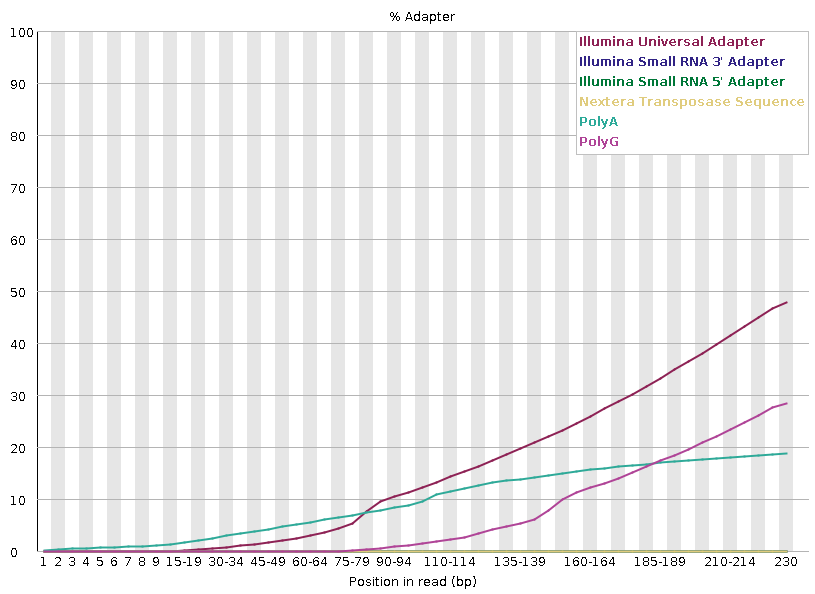
\includegraphics[keepaspectratio]{chapters/../figures/adaptateur_R1_BC76_bf_trimm.png}}

}

\subcaption{\label{fig-before}before trimming}

\end{minipage}%
%
\begin{minipage}{0.50\linewidth}

\centering{

\pandocbounded{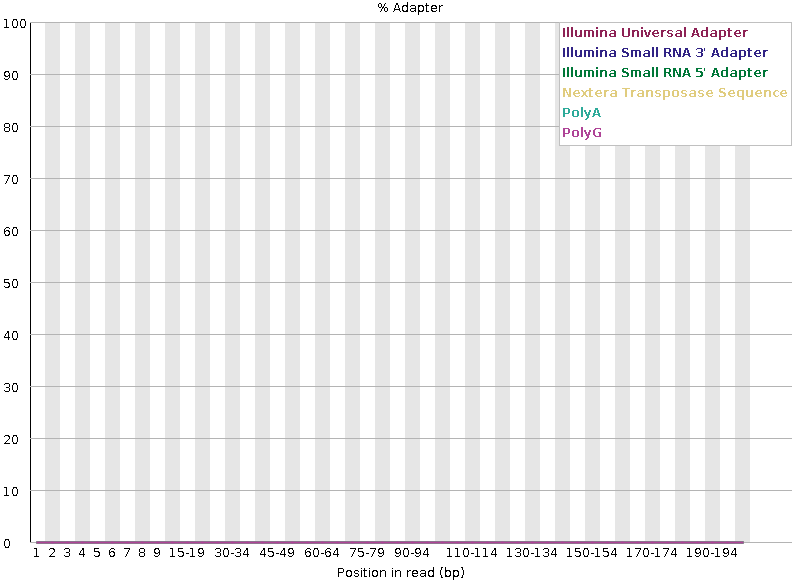
\includegraphics[keepaspectratio]{chapters/../figures/adaptateur_R1_BC76_after_trimm.png}}

}

\subcaption{\label{fig-after}after trimming}

\end{minipage}%

\caption{\label{fig-adaptateur}Artifacts content of the sublibrary
BC\_0076 before and after trimming with Cutadapt and Fastp}

\end{figure}%

\emph{The adapter content analysis shows the presence of various
sequencing artifacts in the raw data (example of BC\_0076). In the
before trimming plot (Figure~\ref{fig-before}), distinct patterns are
visible: polyG stretches (pink), polyA tails (cyan), and Illumina
adapter sequences (purple). After trimming (Figure~\ref{fig-after}),
these artifacts are effectively removed, resulting in clean sequence
data suitable for downstream analysis. The successful elimination of
these technical artifacts demonstrates the effectiveness of the trimming
pipeline in improving data quality.}

\begin{table}

\caption{\label{tbl-summary-trimming}Summary of sequence metrics before
and after trimming of each sublibrary with Cutadapt and Fastp (R1 read
length metrics)}

\begin{minipage}{\linewidth}

\begin{longtable}[]{@{}
  >{\raggedright\arraybackslash}p{(\linewidth - 10\tabcolsep) * \real{0.2131}}
  >{\raggedright\arraybackslash}p{(\linewidth - 10\tabcolsep) * \real{0.1475}}
  >{\raggedright\arraybackslash}p{(\linewidth - 10\tabcolsep) * \real{0.1475}}
  >{\raggedright\arraybackslash}p{(\linewidth - 10\tabcolsep) * \real{0.1475}}
  >{\raggedright\arraybackslash}p{(\linewidth - 10\tabcolsep) * \real{0.1475}}
  >{\raggedright\arraybackslash}p{(\linewidth - 10\tabcolsep) * \real{0.1967}}@{}}
\toprule\noalign{}
\begin{minipage}[b]{\linewidth}\raggedright
Sample Name
\end{minipage} & \begin{minipage}[b]{\linewidth}\raggedright
BC\_0076
\end{minipage} & \begin{minipage}[b]{\linewidth}\raggedright
BC\_0077
\end{minipage} & \begin{minipage}[b]{\linewidth}\raggedright
BC\_0079
\end{minipage} & \begin{minipage}[b]{\linewidth}\raggedright
BC\_0080
\end{minipage} & \begin{minipage}[b]{\linewidth}\raggedright
\(Mean\)/Total
\end{minipage} \\
\midrule\noalign{}
\endhead
\bottomrule\noalign{}
\endlastfoot
R1 length before trimming & 241bp & 241bp & 241bp & 241bp & \(241bp\) \\
R1 length after trimming & 127bp & 157bp & 152bp & 132bp & \(142bp\) \\
R1 number of sequences before trimming & 631.4M & 325.5M & 379.1M &
397.7M & \textbf{1733.7M} \\
R1 number of sequences after trimming & 450.8M & 248.4M & 285.2M &
300.1M & \textbf{1284.5M} \\
Change in number of sequences & -28.6\% & -23.7\% & -24.8\% & -24.5\% &
\textbf{-25.4\%} \\
\end{longtable}

\end{minipage}%

\end{table}%

The trimming process successfully removed various sequencing artifacts
and improved data quality for downstream analysis. The preprocessing
pipeline eliminated template-switching oligo (TSO) sequences, polyG
stretches (NovaSeq-specific artifacts), polyA tails, and adapter
sequences from the raw sequencing data (Figure~\ref{fig-adaptateur},
Table~\ref{tbl-summary-trimming}). This cleaning step was essential for
accurate gene expression quantification and reliable single-cell
analysis.

\subsubsection{Trimming Efficiency and Data
Retention}\label{trimming-efficiency-and-data-retention}

The trimming process resulted in an average reduction of 25.4\% in the
total number of sequences across all sublibraries, from 1,733.7 million
to 1,284.5 million reads (Table~\ref{tbl-summary-trimming}). This
reduction rate is within the expected range for single-cell RNA-seq data
and indicates effective removal of low-quality sequences while
preserving the majority of informative reads. The final dataset of 1.284
billion reads provides substantial sequencing depth for robust analysis.

\subsubsection{Sub-library Size Variations and Their
Implications}\label{sub-library-size-variations-and-their-implications}

The four sublibraries showed notable size differences before trimming,
ranging from 325.5 million reads (BC\_0077) to 631.4 million reads
(BC\_0076) (Table~\ref{tbl-summary-trimming}). These variations likely
reflect differences in library preparation efficiency and sequencing
performance across the flowcell. The largest library (BC\_0076)
exhibited the most significant reduction in read length after trimming
(from 241bp to 127bp), suggesting higher levels of sequencing artifacts
in this sublibrary (Table~\ref{tbl-summary-trimming}).

\subsubsection{Quality Improvements and Technical
Considerations}\label{quality-improvements-and-technical-considerations}

The trimming process revealed interesting patterns across sublibraries.
BC\_0076 and BC\_0080 showed the most pronounced reductions in R1 read
length, which may indicate higher initial quality of these libraries
requiring more aggressive trimming to remove artifacts while maintaining
better overall data integrity.

BC\_0076 specifically showed earlier and more prominent polyG artifacts,
likely due to reagent depletion during sequencing that led to increased
G nucleotide incorporation errors. This phenomenon is common in NovaSeq
sequencing runs where the largest libraries may experience reagent
exhaustion, resulting in higher error rates and more artifacts that
require removal during trimming. Despite these technical challenges, the
trimming process successfully mitigated these artifacts, resulting in
high-quality data suitable for downstream analysis.

\begin{tcolorbox}[enhanced jigsaw, arc=.35mm, colbacktitle=quarto-callout-tip-color!10!white, rightrule=.15mm, title=\textcolor{quarto-callout-tip-color}{\faLightbulb}\hspace{0.5em}{Recommendations for Future Experiments}, coltitle=black, bottomrule=.15mm, left=2mm, opacityback=0, colback=white, toprule=.15mm, toptitle=1mm, titlerule=0mm, breakable, bottomtitle=1mm, opacitybacktitle=0.6, colframe=quarto-callout-tip-color-frame, leftrule=.75mm]

The observed size variations between sublibraries highlight the
importance of balanced library preparation for optimal sequencing
efficiency. Libraries of unequal sizes can lead to differential reagent
consumption and varying quality across the flowcell. Future experiments
should aim for more balanced library sizes to minimize technical
artifacts and ensure consistent quality across all sublibraries.

\end{tcolorbox}

\subsubsection{MultiQC Report R1 Before
Trimming}\label{multiqc-report-r1-before-trimming}

Click to view MultiQC report R1 before trimming

\subsubsection{MultiQC Report R1 After
Trimming}\label{multiqc-report-r1-after-trimming}

Click to view MultiQC report R1 after trimming

\subsubsection{MultiQC Report R2 Before
Trimming}\label{multiqc-report-r2-before-trimming}

Click to view MultiQC report R2 before trimming

\subsubsection{MultiQC Report R2 After
Trimming}\label{multiqc-report-r2-after-trimming}

Click to view MultiQC report R2 after trimming

\subsection{Transcriptome Description after STARsolo
processing}\label{transcriptome-description-after-starsolo-processing}

Following the successful preprocessing and trimming of our sequencing
data, we performed alignment against the reference genome of \emph{P.
brassicacearum R401} (Figure~\ref{fig-genome}). The barcode reading and
quantification by STARsolo provided comprehensive quality metrics and
mapping statistics.

\begin{table}

\caption{\label{tbl-starsolo-comprehensive}Summary of metrics obtained
with STARsolo after barcode-UMI reading and alignment with the reference
genome of \emph{P. brassicacearum R401}}

\begin{minipage}{\linewidth}

\begin{longtable}[]{@{}
  >{\raggedright\arraybackslash}p{(\linewidth - 2\tabcolsep) * \real{0.7049}}
  >{\raggedright\arraybackslash}p{(\linewidth - 2\tabcolsep) * \real{0.2951}}@{}}
\toprule\noalign{}
\begin{minipage}[b]{\linewidth}\raggedright
Metric
\end{minipage} & \begin{minipage}[b]{\linewidth}\raggedright
Count/Percentage
\end{minipage} \\
\midrule\noalign{}
\endhead
\bottomrule\noalign{}
\endlastfoot
\textbf{Total Reads Processed} & 1,284,475,633 \\
\textbf{N\_reads with valid barcodes} & 1,099,327,755
(\textbf{85.58\%}) \\
- Exact Barcode Match & -\textgreater{} 1,046,121,284
(\textbf{81.44\%}) \\
- Single Mismatch Barcode & -\textgreater{} 53,206,471
(\textbf{4.14\%}) \\
\textbf{Q30 Bases in RNA reads} & 95.79\% \\
\textbf{Q30 Bases in CB+UMI} & 95.51\% \\
\textbf{Unique Gene Mapping} & 34,593,349 (2.69\%) \\
\textbf{Unique + Multiple Gene Mapping} & 971,519,404 (75.64\%) \\
\textbf{Total Genes Detected} & 6,035 on the total of 6,249 genes
(96.57\%) \\
\textbf{Cell Barcodes Detected} & 699,355 \\
\textbf{N\_umi} & 36,565,214 \\
\textbf{Sequencing Saturation} & 0.97\% \\
\end{longtable}

\end{minipage}%

\end{table}%

\emph{Metrics obtained with STARsolo after barcode-UMI reading and
alignment with the reference genome of }P. brassicacearum R401\emph{.}

The STARsolo analysis processed the 1.284 billion trimmed reads and
successfully identified 1.099 billion reads with valid barcodes (85.58\%
of total reads), demonstrating excellent barcode quality
(Table~\ref{tbl-starsolo-comprehensive}). Among these, 81.44\% had exact
barcode matches and 4.14\% had single mismatches, indicating robust cell
identification. The sequencing quality was outstanding with Q30 scores
above 95\% for both RNA reads and barcode/UMI sequences. This high
percentage of valid barcodes falls within the expected range of 70-90\%
for successful experiments, as recommended by Gaisser et al.~(2024)
(\textsuperscript{\citeproc{ref-gaisser2024}{32}}), indicating excellent
library preparation and barcoding efficiency with no significant issues
in the protocol optimization.

Gene mapping analysis revealed that 75.64\% of reads mapped to genes,
with 2.69\% showing unique mapping and the remainder showing multiple
mapping, which is typical for bacterial genomes with overlapping genes
and repeated sequences. The fraction of uniquely aligned reads (2.69\%)
falls within the expected range of 3-12\% for bacterial samples (Gaisser
et al.~(\textsuperscript{\citeproc{ref-gaisser2024}{32}})). This value
is influenced by the species-specific characteristics and experimental
conditions.

A total of 6,035 genes were detected across 699,355 unique cell
barcodes, representing 96.6\% of the 6,249 genes
(Figure~\ref{fig-genome}) annotated in the \emph{P. brassicacearum R401}
genome, with one gene being automatically ignored by STARsolo due to
poor annotation.

The sequencing saturation, calculated as:

\[ Sequencing\ Saturation = 1 - \frac{N_{\text{umi}}}{N_{\text{reads with valid barcodes}}} = 1 - \frac{36,565,214}{1,099,327,755} = 0.97\% \]

\begin{itemize}
\tightlist
\item
  Where:

  \begin{itemize}
  \tightlist
  \item
    \(N_{\text{umi}}\) = number of unique molecules detected, distinct
    combinations of Cell Barcode (CB) / UMI / gene
  \item
    \(N_{\text{reads}}\) = total number of reads with valid CB/UMI/gene
    combinations
  \end{itemize}
\end{itemize}

\begin{tcolorbox}[enhanced jigsaw, arc=.35mm, colbacktitle=quarto-callout-warning-color!10!white, rightrule=.15mm, title=\textcolor{quarto-callout-warning-color}{\faExclamationTriangle}\hspace{0.5em}{Warning}, coltitle=black, bottomrule=.15mm, left=2mm, opacityback=0, colback=white, toprule=.15mm, toptitle=1mm, titlerule=0mm, breakable, bottomtitle=1mm, opacitybacktitle=0.6, colframe=quarto-callout-warning-color-frame, leftrule=.75mm]

This very low saturation indicates that we have captured only a small
fraction of the total unique molecules in the transcriptome. According
to Gaisser et
al.~(2024)\textsuperscript{\citeproc{ref-gaisser2024}{32}}, a sequencing
saturation of \textless0.5 may indicate that more sequencing is required
to capture all barcoded transcripts in the library, with a saturation
value of \textgreater= 0.7 typically indicating sufficient coverage. Our
saturation value of 0.97\% falls well below these recommended
thresholds, suggesting that \textbf{our current sequencing depth may not
be sufficient to capture the full complexity of the transcriptome}.
While the current sequencing depth of 1.284 billion reads provides
substantial coverage, the low saturation indicates that we could
potentially benefit from deeper sequencing to capture more unique
transcripts and achieve better coverage of the transcriptional
landscape.

\end{tcolorbox}

\begin{figure}

\begin{minipage}{0.50\linewidth}

\centering{

\pandocbounded{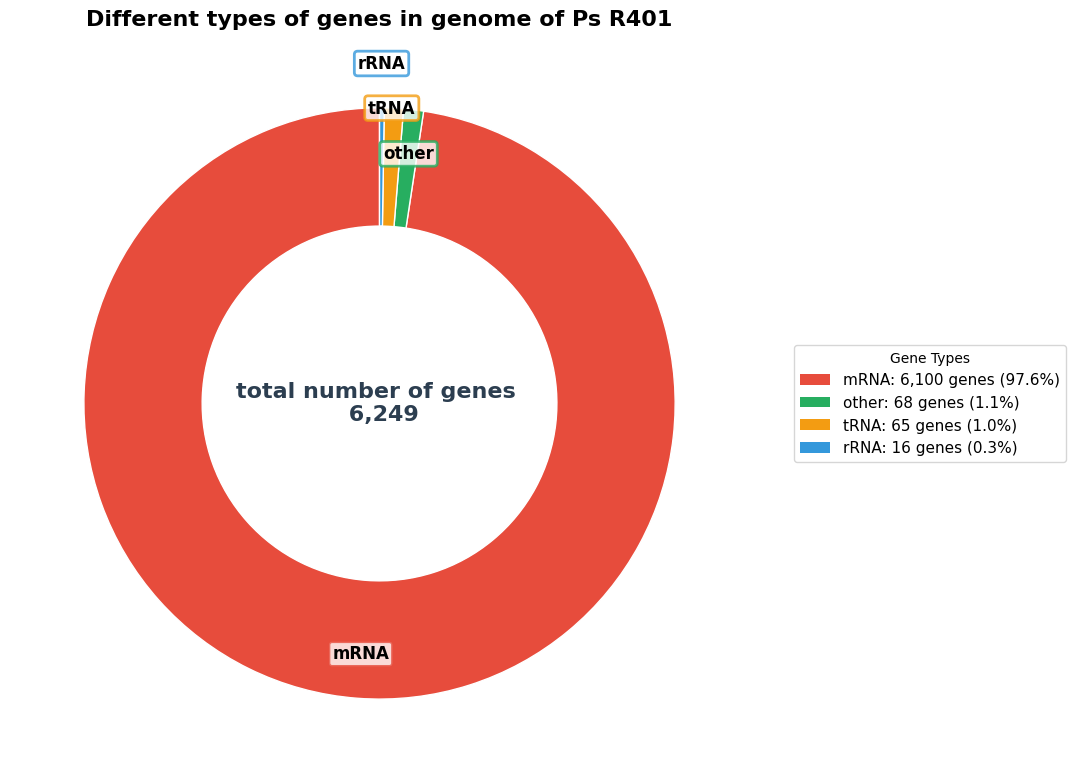
\includegraphics[keepaspectratio]{chapters/../figures/genome_description.png}}

}

\subcaption{\label{fig-genome}genome}

\end{minipage}%
%
\begin{minipage}{0.50\linewidth}

\centering{

\pandocbounded{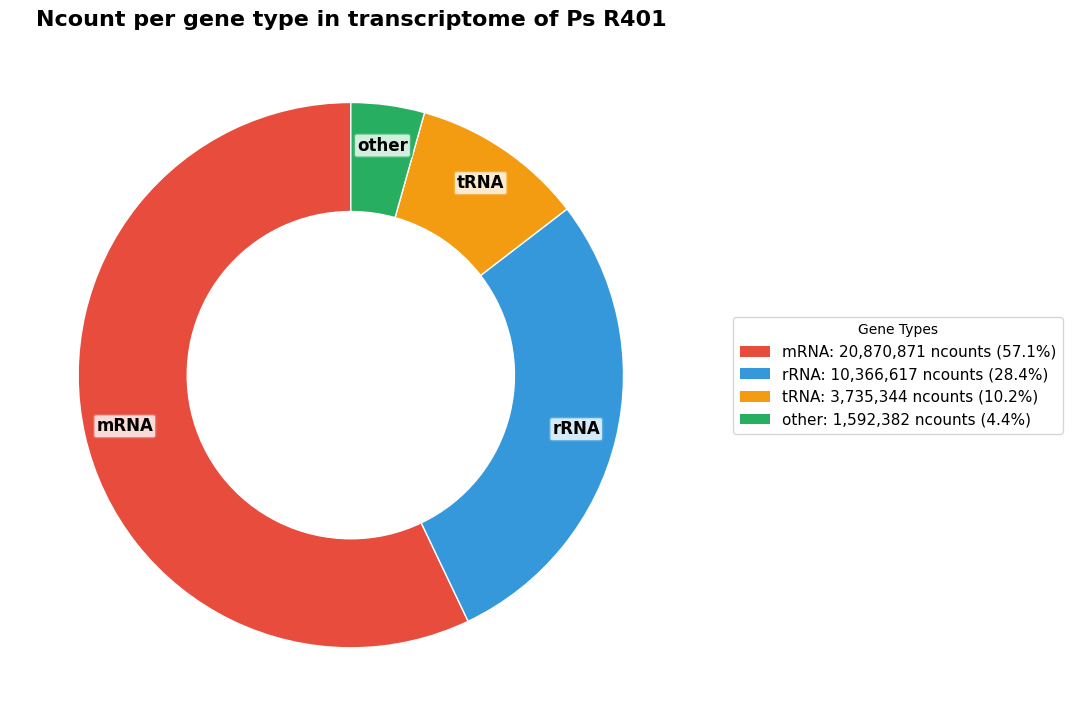
\includegraphics[keepaspectratio]{chapters/../figures/transcriptome_description.png}}

}

\subcaption{\label{fig-transcriptome}transcriptome}

\end{minipage}%

\caption{\label{fig-genome-transcriptome}Compositional analysis of
\emph{P. brassicacearum} R401 genome annotation and transcriptome
distribution of different RNA types}

\end{figure}%

The genome and transcriptome composition analysis reveals the
distribution of different RNA types in our \emph{P. brassicacearum}
sample. In the
\href{https://www.ncbi.nlm.nih.gov/datasets/gene/GCA_030064105.1/}{annotated}
genome of \emph{P. brassicacearum} R401, we identified 6,100 mRNA genes
(97.6\% of total genes), 65 tRNA genes, 16 rRNA genes (0.3\% of the
genome) and 68 other genes. However, in the transcriptome analysis of
our 36,565,214 UMIs, the distribution shows a different pattern: 57.1\%
correspond to mRNA transcripts (21 millions), while 28.4\% are rRNA
transcripts (representing approximately 10 millions UMIs), 10.2 \% are
tRNA transcripts (representing approximately 4 millions UMIs) and 4.4\%
are other genes (representing approximately 1.5 millions UMIs). This
distribution concords with the well-established observation that rRNA
and tRNA transcripts represent a large proportion of the bacterial
transcriptome despite constituting only a small fraction of the genome,
due to their high transcriptional activity and
stability\textsuperscript{\citeproc{ref-nishimura2025}{26}}.

STARsolo detected 699,355 out of 820,800 possible barcode combinations.
Given that our sublibrary was designed to target approximately 3,000
cells, the observed number of barcodes is within the expected range. The
presence of additional barcodes likely represents contamination that can
occur throughout the protocol, including potential contamination in the
source oligonucleotide plates. To identify genuine cells among the total
barcode population, STARsolo employs a knee plot strategy (see
supplementary data for associated results). As recommended in the
literature (Gaisser et
al.~(2024)\textsuperscript{\citeproc{ref-gaisser2024}{32}}), we chose to
apply our own filtering criteria rather than using STARsolo's default
KneePant method, which would have resulted in approximately 27,000
cells. This decision was based on the concern that the KneePant method
might eliminate stressed cells that could have lower quality metrics
compared to non-stressed cells, potentially biasing our division of
labor analysis by removing biologically relevant subpopulations.

Despite the low sequencing depth indicated by the saturation value, we
will assess whether the signal is sufficient for division of labor
analysis. However, before proceeding with this assessment, it is
necessary to filter the barcodes to retain only genuine cells, as the
current dataset contains a large number of contaminating barcodes that
could mask the biological signal of interest.

\subsection{Cell Filtering Strategy}\label{cell-filtering-strategy}

\subsection{Filtering of cells based on UMI
counts}\label{filtering-of-cells-based-on-umi-counts}

\subsubsection{Filtering minimum 100 UMI per Barcode
Cell}\label{filtering-minimum-100-umi-per-barcode-cell}

\begin{figure}

\begin{minipage}{0.50\linewidth}

\centering{

\pandocbounded{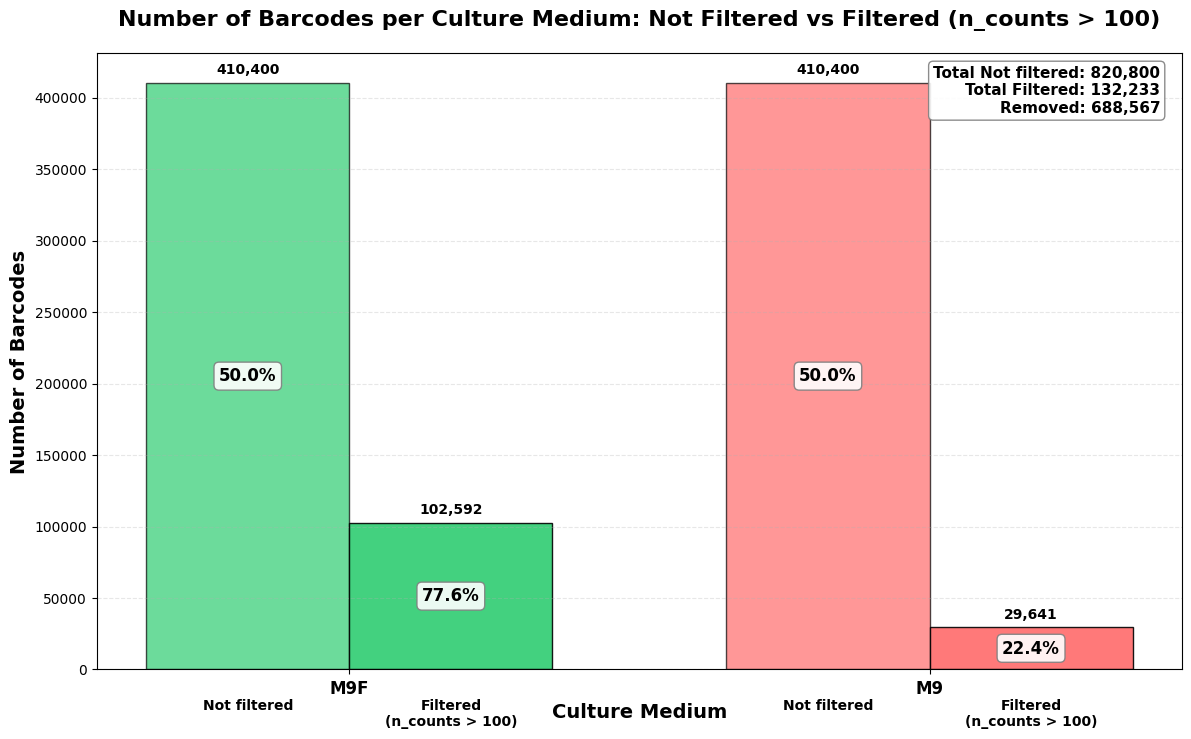
\includegraphics[keepaspectratio]{chapters/../figures/filter_100UMIs_barplot.png}}

}

\subcaption{\label{fig-barplot}Barplot of the number of UMI per cell
before and after filtering}

\end{minipage}%
%
\begin{minipage}{0.50\linewidth}

\centering{

\pandocbounded{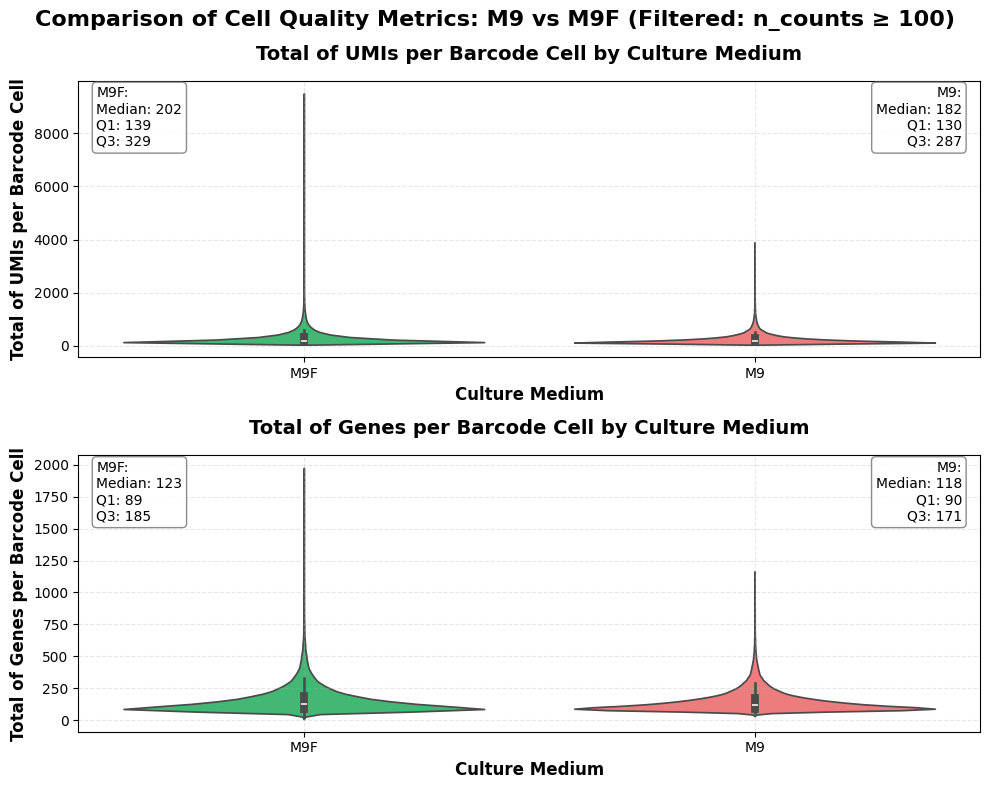
\includegraphics[keepaspectratio]{chapters/../figures/violinplot_100UMIs.png}}

}

\subcaption{\label{fig-violin}Violin plot of the number of UMI and genes
per Barcode Cell after a filtering at 100 UMIs}

\end{minipage}%
\newline
\begin{minipage}{\linewidth}

\centering{

\pandocbounded{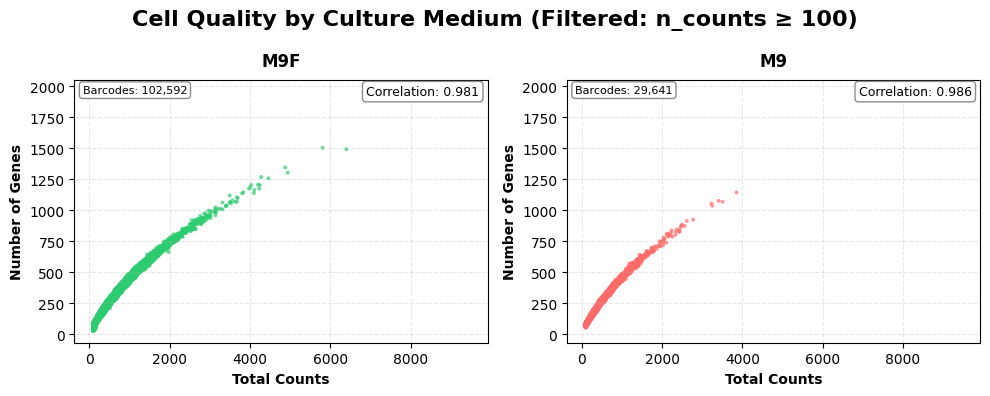
\includegraphics[keepaspectratio]{chapters/../figures/filter_100UMI_scatter_CutureMedium.png}}

}

\subcaption{\label{fig-scatter}Scatter plot of the number of UMI per
cell after 100 UMIs per Barcode Cell filtering}

\end{minipage}%
\newline
\begin{minipage}{\linewidth}

\centering{

\pandocbounded{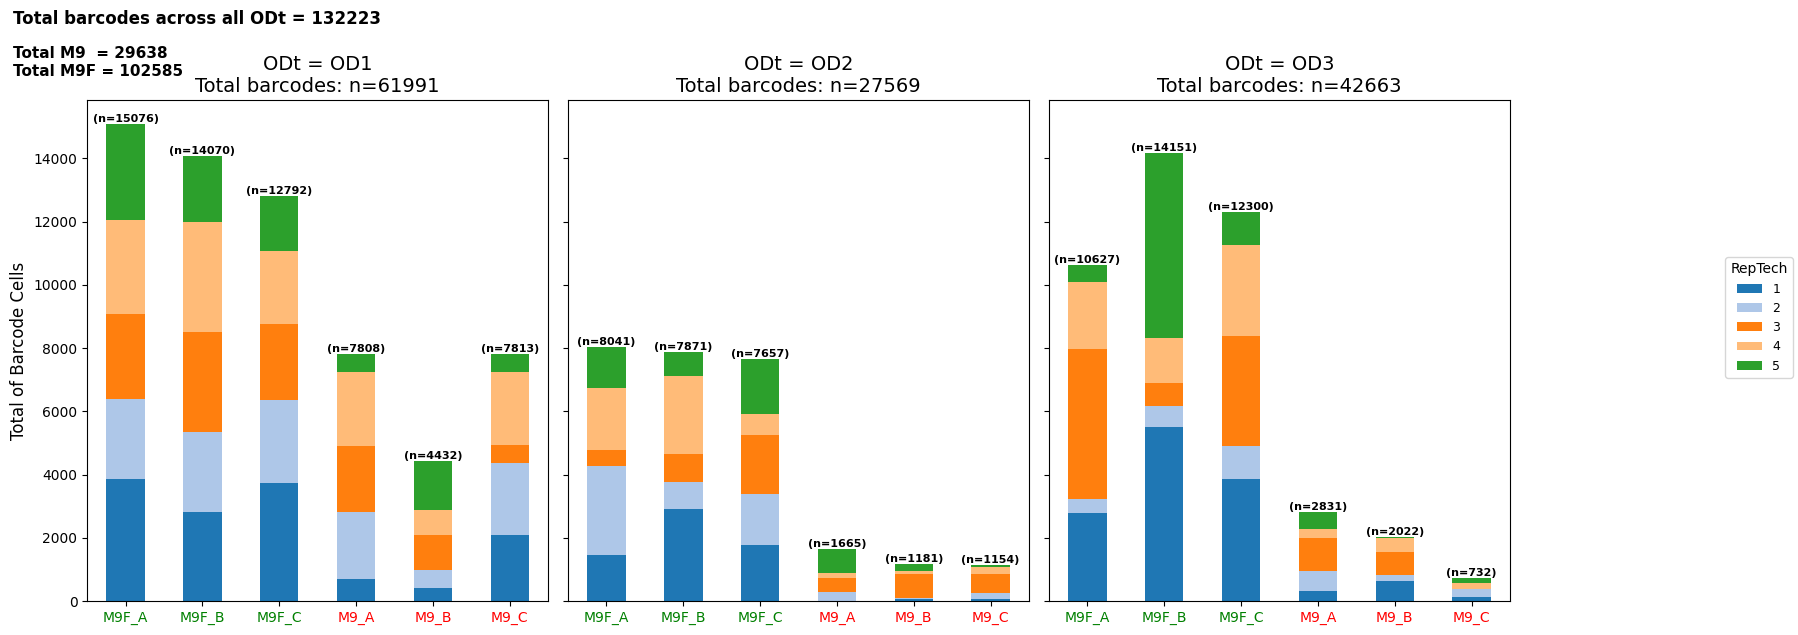
\includegraphics[keepaspectratio]{chapters/../figures/splitplot_barcodes_100UMIs.png}}

}

\subcaption{\label{fig-splitplot-barcodes}Total of barcodes for each
biological replicate after filtering at 100 UMIs}

\end{minipage}%

\caption{\label{fig-filter_100UMI}Filtering of cells with less than 100
UMI per cell}

\end{figure}%

\subsubsection{Final Filtering}\label{final-filtering}

\begin{figure}

\centering{

\pandocbounded{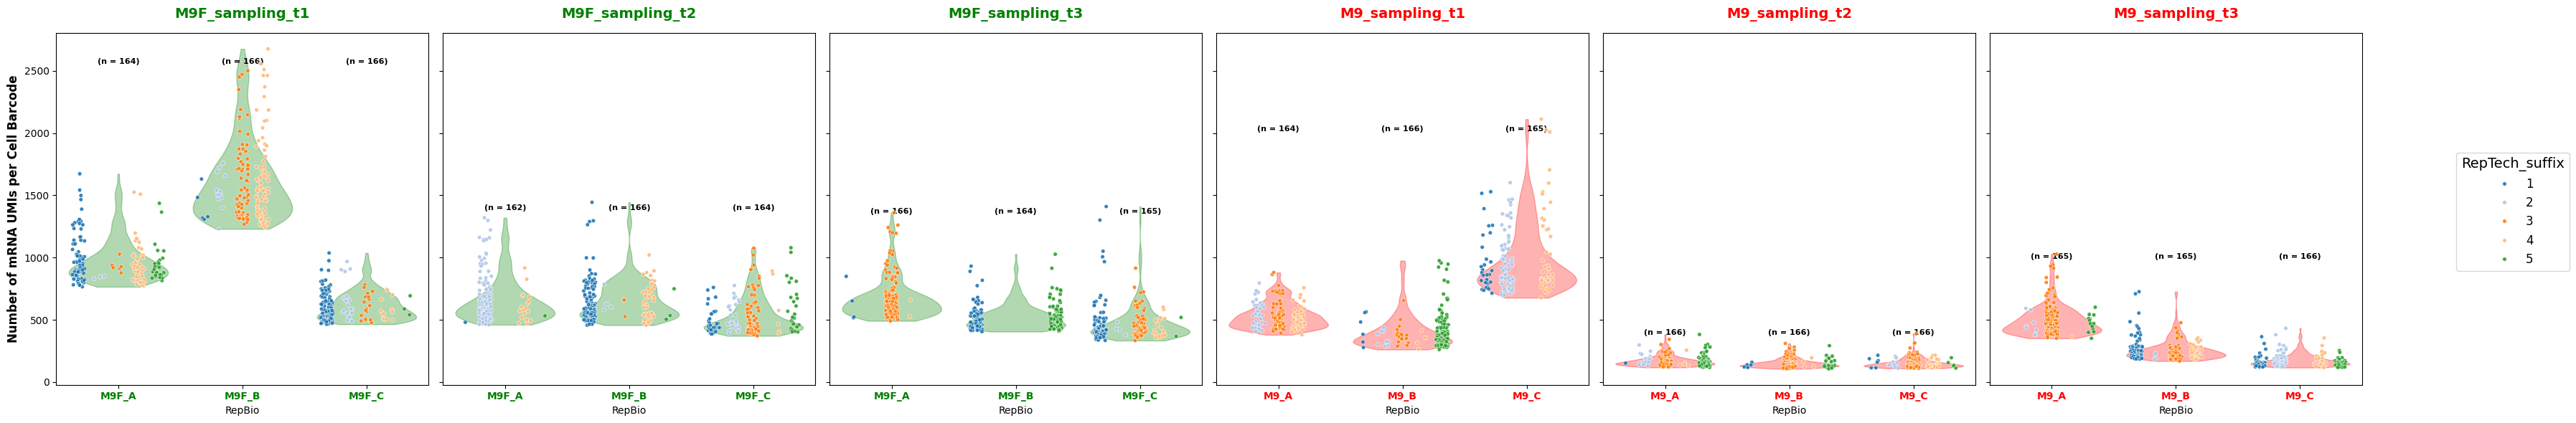
\includegraphics[keepaspectratio]{chapters/../figures/mRNA_Genes_filtered.png}}

}

\caption{\label{fig-filtered_mRNA_violin}}

\end{figure}%

le choix de filtration sera discuté apres

because the reads depth is different between : Stress condition (M9F)
and non-stress condition (M9) et also between the 3 timepoints (T1, T2,
T3) (voir figure, reuslttas comme deja observé chez )

, which typically corresponds to the mRNA proportion in the library

attention duplication des reads

serait bien de tester chaque sublirbai starsolo independant

The low saturation may be partially explained by the high complexity of
the bacterial transcriptome and the large number of unique cell barcode
combinations detected (699,355).

Our results align well with the expected performance metrics for
single-cell RNA-seq in bacteria.

It is important to note that preliminary STARsolo tests without trimming
yielded saturation values 0.94 \textbf{\textgreater{} 0.7}, which would
have met the Gaisser et
al.~(\textsuperscript{\citeproc{ref-gaisser2024}{32}}) recommendation
for adequate sequencing depth. However, these elevated saturation values
were not due to superior sequencing quality but rather to less
effectively trimmed reads that artificially affected the saturation
ratio. The lower saturation observed in our final analysis with proper
trimming (0.0097) actually reflects more accurate data quality
assessment, as the trimming process removed sequencing artifacts and
low-quality reads that would have otherwise inflated the saturation
metric. This observation suggests that the interpretation of saturation
values in the Gaisser et
al.(\textsuperscript{\citeproc{ref-gaisser2024}{32}}) study may need
revision, as their trimming protocol reportedly left approximately 10\%
of TSO sequences remaining, which could have artificially inflated their
saturation metrics. While our saturation value of 0.97\% falls well
below their recommended threshold of \textgreater0.7, this difference
likely reflects the superior quality of our trimming protocol rather
than inadequate sequencing depth. The low saturation value (0.97\%)
indicates minimal redundancy in our sequencing data, suggesting that a
substantial portion of the transcriptome remains unexplored. This
implies that deeper sequencing could potentially capture additional
unique transcripts and provide more comprehensive coverage of the
transcriptional landscape.

peut etre devoir verifier les 4 biblioteques pour comprendre les
differences de duplication et voir si differences de satureation

For our division of labor analysis focusing on mRNA expression patterns,
these highly abundant non-coding RNAs will need to be filtered out to
avoid masking subtle transcriptional differences between subpopulations.
This information is crucial for understanding the transcriptional
landscape and identifying potential division of labor patterns, as
different RNA types may be differentially expressed across
subpopulations.

\textbf{Key considerations for division of labor analysis:} - The choice
of filtering threshold can significantly impact the detection of rare
subpopulations - Housekeeping genes and rRNA content may provide
insights into growth rate variations across cells - Technical replicates
may need to be pooled or analyzed separately depending on experimental
design

\bookmarksetup{startatroot}

\chapter{Discussion}\label{discussion}

We applied microSPLiT to P. brassicacearum growing in two different
conditions in rich medium (M9F) and in minimal medium (M9).

-d'autres methodes de filtrage , log log comme dans\ldots{}

While other tools exist for alignment and barcode reading in
SPLiT-seq/microSPLiT protocols, such as
Kallisto\textsuperscript{\citeproc{ref-bray2016}{45},\citeproc{ref-sullivan2025}{46}},
The pipeline could be further improved with additional quality
verification steps and implementation of workflow management systems
such as Nextflow and nf-core for enhanced reproducibility and
scalability.

\begin{verbatim}
-   different other tools existe comme pour alignement et lecture des barcodes SPLiTseq/ microSPliT comme Kallisto [@bray2016], [@sullivan2025] mais d'apres le benchmarking de le plus rapide, reproductible est starsolo [@kuijpers2024]
\end{verbatim}

pleins parametre pour etre change, unique alignement peut de rRNA je
trouve par rapport a autre articles

To remove empty and low gene detection barcodes, we applied the ``knee''
detection filter previously described in Brettner et al.~202435. These
quality-thresholded gene-by-barcode matrices were then converted to the
R datatype, Seurat Objects, using the Seurat R package for further
analyses83.

\begin{itemize}
\tightlist
\item
  biais de la methode
\item
  coloration fluorescences pour voir marqueur , cell states , i
\end{itemize}

-agotation oiu pas

-discuter du pipeline bac -voir

\begin{itemize}
\item
  recepetion tardives des resultats
\item
  mis beaucoup de temps pour le trimming ( 1mois) le temps de comprendre
  la structure de la librairie et
\item
\item
\item
  analyse temporelle , metabolique , bulkRNAseq
\item
  utilisation pour capturer specifique mRNA (voir article : 2 methodes
  existes ; et apres aussi peut etre fait )
\item
  mais je pense deja bioinformatiquement on peut faire des choses pour
  ameliorer reads utilisables
\item
  comparer avec differentes methodes de single cell RNA seq, voir si on
  observe toujours la meme chose ou pas
\item
  versionnement des outils utilisés (renv , singularity, conda)
\item
  rapport fait un template pour rendu propre
\item
\end{itemize}

autres outils pourrait etre ajouter dans le pipeline comme BarQC
alternative à Starsolo pour meilleur la lecture des barcodes (en
considerant utilisant des positions non fixe (CIGAR motif) et evaluer la
qualité UMIs et
repartitions\textsuperscript{\citeproc{ref-rossello}{47}},

pour la qualité et contamination : centriguge et
recentrifuge\textsuperscript{\citeproc{ref-martuxed2019}{48},\citeproc{ref-kim2016}{49}}

meme si moins de risque de contamination car cellules fixé \ldots{}
(deve

\begin{itemize}
\tightlist
\item
  Nextflow pour le trimming, QC , et STARsolo serait une bonne idée , et
  barQC ; pourrait etre utile pour la communauté
\end{itemize}

-autono -gestion des datas tailles des \#\# Interpretation of Key
Findings

\subsection{Division of Labor
Mechanisms}\label{division-of-labor-mechanisms}

\subsection{Biological Significance}\label{biological-significance}

\subsection{Technical Considerations}\label{technical-considerations}

\section{Comparison with Existing
Literature}\label{comparison-with-existing-literature}

\subsection{Similarities with Previous
Studies}\label{similarities-with-previous-studies}

\subsection{Novel Insights}\label{novel-insights}

\subsection{Discrepancies and Their
Implications}\label{discrepancies-and-their-implications}

\section{Methodological Strengths and
Limitations}\label{methodological-strengths-and-limitations}

\subsection{Technical Advantages}\label{technical-advantages}

\subsection{Potential Limitations}\label{potential-limitations}

\subsection{Future Methodological
Improvements}\label{future-methodological-improvements}

\section{Biological Implications}\label{biological-implications}

\subsection{Ecological Significance}\label{ecological-significance}

\subsection{Evolutionary Perspectives}\label{evolutionary-perspectives}

\subsection{Potential Applications}\label{potential-applications}

\section{Future Research Directions}\label{future-research-directions}

\subsection{Open Questions}\label{open-questions}

\subsection{Suggested Follow-up
Studies}\label{suggested-follow-up-studies}

\subsection{Technical Improvements}\label{technical-improvements}

\section{Conclusion}\label{conclusion}

\bookmarksetup{startatroot}

\chapter{Conclusion and Future Work}\label{conclusion-and-future-work}

\section{Summary of Main Findings}\label{summary-of-main-findings}

\subsection{Key Discoveries}\label{key-discoveries}

\subsection{Methodological
Contributions}\label{methodological-contributions}

\subsection{Biological Insights}\label{biological-insights}

\section{Impact on the Field}\label{impact-on-the-field}

\subsection{Contribution to Single-cell RNA-seq
Methodology}\label{contribution-to-single-cell-rna-seq-methodology}

\subsection{Contribution to Pseudomonas
Research}\label{contribution-to-pseudomonas-research}

\subsection{Broader Implications for Microbial
Ecology}\label{broader-implications-for-microbial-ecology}

\section{Future Research Directions}\label{future-research-directions-1}

\subsection{Technical Improvements}\label{technical-improvements-1}

\subsection{Biological Questions to
Address}\label{biological-questions-to-address}

\subsection{Potential Applications}\label{potential-applications-1}

\section{Final Remarks}\label{final-remarks}

\section{References}\label{references}

\clearpage
% Désactiver l'inclusion des prochaines figures et tableaux dans les listes
\captionsetup[figure]{list=false}
\captionsetup[table]{list=false}

\bookmarksetup{startatroot}

\chapter*{Bibliography}\label{bibliography}
\addcontentsline{toc}{chapter}{Bibliography}

\markboth{Bibliography}{Bibliography}

\phantomsection\label{refs}
\begin{CSLReferences}{0}{0}
\bibitem[\citeproctext]{ref-cooper2018}
\CSLLeftMargin{1. }%
\CSLRightInline{Cooper, G. A. \& West, S. A.
\href{https://doi.org/10.1038/s41559-018-0564-9}{Division of labour and
the evolution of extreme specialization}. \emph{Nature Ecology \&
Evolution} \textbf{2}, 1161--1167 (2018).}

\bibitem[\citeproctext]{ref-giri2019}
\CSLLeftMargin{2. }%
\CSLRightInline{Giri, S., Waschina, S., Kaleta, C. \& Kost, C.
\href{https://doi.org/10.1016/j.jmb.2019.06.023}{Defining division of
labor in microbial communities}. \emph{Journal of Molecular Biology}
\textbf{431}, 4712--4731 (2019).}

\bibitem[\citeproctext]{ref-taborsky2025}
\CSLLeftMargin{3. }%
\CSLRightInline{Taborsky, M., Fewell, J. H., Gilles, R. \& Taborsky, B.
\href{https://doi.org/10.1098/rstb.2023.0261}{Division of labour as key
driver of social evolution}. \emph{Philosophical Transactions of the
Royal Society B: Biological Sciences} \textbf{380}, 20230261 (2025).}

\bibitem[\citeproctext]{ref-rafieenia2022}
\CSLLeftMargin{4. }%
\CSLRightInline{Rafieenia, R., Atkinson, E. \& Ledesma-Amaro, R.
\href{https://doi.org/10.1016/j.copbio.2022.102706}{Division of labor
for substrate utilization in natural and synthetic microbial
communities}. \emph{Current Opinion in Biotechnology} \textbf{75},
102706 (2022).}

\bibitem[\citeproctext]{ref-mataigne2021}
\CSLLeftMargin{5. }%
\CSLRightInline{Mataigne, V., Vannier, N., Vandenkoornhuyse, P. \&
Hacquard, S. \href{https://doi.org/10.3389/fmicb.2021.780469}{Microbial
systems ecology to understand cross-feeding in microbiomes}.
\emph{Frontiers in Microbiology} \textbf{12}, (2021).}

\bibitem[\citeproctext]{ref-mataigne2022}
\CSLLeftMargin{6. }%
\CSLRightInline{Mataigne, V., Vannier, N., Vandenkoornhuyse, P. \&
Hacquard, S.
\href{https://doi.org/10.1186/s40168-022-01383-z}{Multi-genome metabolic
modeling predicts functional inter-dependencies in the arabidopsis root
microbiome}. \emph{Microbiome} \textbf{10}, 217 (2022).}

\bibitem[\citeproctext]{ref-estrela2016}
\CSLLeftMargin{7. }%
\CSLRightInline{Estrela, S., Kerr, B. \& Morris, J. J.
\href{https://doi.org/10.1016/j.mib.2016.04.007}{Transitions in
individuality through symbiosis}. \emph{Current Opinion in Microbiology}
\textbf{31}, 191--198 (2016).}

\bibitem[\citeproctext]{ref-adkins-jablonsky2021}
\CSLLeftMargin{8. }%
\CSLRightInline{Adkins-Jablonsky, S. J., Clark, C. M., Papoulis, S. E.,
Kuhl, M. D. \& Morris, J. J.
\href{https://doi.org/10.1073/pnas.2109813118}{Market forces determine
the distribution of a leaky function in a simple microbial community}.
\emph{Proceedings of the National Academy of Sciences of the United
States of America} \textbf{118}, e2109813118 (2021).}

\bibitem[\citeproctext]{ref-luxf3pez-paguxe1n2025}
\CSLLeftMargin{9. }%
\CSLRightInline{López-Pagán, N. \emph{et al.}
\href{https://doi.org/10.1038/s41564-025-01966-0}{Pseudomonas syringae
subpopulations cooperate by coordinating flagellar and type III
secretion spatiotemporal dynamics to facilitate plant infection}.
\emph{Nature Microbiology} \textbf{10}, 958--972 (2025).}

\bibitem[\citeproctext]{ref-raj2008}
\CSLLeftMargin{10. }%
\CSLRightInline{Raj, A. \& Oudenaarden, A. van.
\href{https://doi.org/10.1016/j.cell.2008.09.050}{Nature, nurture, or
chance: Stochastic gene expression and its consequences}. \emph{Cell}
\textbf{135}, 216--226 (2008).}

\bibitem[\citeproctext]{ref-keren2015}
\CSLLeftMargin{11. }%
\CSLRightInline{Keren, L. \emph{et al.}
\href{https://doi.org/10.1101/gr.191635.115}{Noise in gene expression is
coupled to growth rate}. \emph{Genome Research} \textbf{25}, 1893--1902
(2015).}

\bibitem[\citeproctext]{ref-chowdhury2021}
\CSLLeftMargin{12. }%
\CSLRightInline{Chowdhury, D., Wang, C., Lu, A. \& Zhu, H.
\href{https://doi.org/10.3389/fgene.2021.698910}{Cis-regulatory logic
produces gene-expression noise describing phenotypic heterogeneity in
bacteria}. \emph{Frontiers in Genetics} \textbf{12}, (2021).}

\bibitem[\citeproctext]{ref-lopez2022}
\CSLLeftMargin{13. }%
\CSLRightInline{Lopez, J. G. \& Wingreen, N. S.
\href{https://doi.org/10.7554/eLife.70694}{Noisy metabolism can promote
microbial cross-feeding}. \emph{eLife} \textbf{11}, e70694 (2022).}

\bibitem[\citeproctext]{ref-korshoj2024}
\CSLLeftMargin{14. }%
\CSLRightInline{Korshoj, L. E. \& Kielian, T.
\href{https://doi.org/10.1038/s41467-024-54581-8}{Bacterial single-cell
RNA sequencing captures biofilm transcriptional heterogeneity and
differential responses to immune pressure}. \emph{Nature Communications}
\textbf{15}, 10184 (2024).}

\bibitem[\citeproctext]{ref-knights2021}
\CSLLeftMargin{15. }%
\CSLRightInline{Knights, H. E., Jorrin, B., Haskett, T. L. \& Poole, P.
S. \href{https://doi.org/10.1111/1758-2229.12934}{Deciphering bacterial
mechanisms of root colonization}. \emph{Environmental Microbiology
Reports} \textbf{13}, 428--444 (2021).}

\bibitem[\citeproctext]{ref-getzke2023}
\CSLLeftMargin{16. }%
\CSLRightInline{Getzke, F. \emph{et al.}
\href{https://doi.org/10.1073/pnas.2221508120}{Cofunctioning of
bacterial exometabolites drives root microbiota establishment}.
\emph{Proceedings of the National Academy of Sciences} \textbf{120},
e2221508120 (2023).}

\bibitem[\citeproctext]{ref-jian2024}
\CSLLeftMargin{17. }%
\CSLRightInline{Jian, Y. \emph{et al.}
\href{https://doi.org/10.1038/s44319-023-00023-3}{How plants manage
pathogen infection}. \emph{EMBO reports} \textbf{25}, 31--44 (2024).}

\bibitem[\citeproctext]{ref-dodds2024}
\CSLLeftMargin{18. }%
\CSLRightInline{Dodds, P. N., Chen, J. \& Outram, M. A.
\href{https://doi.org/10.1093/plcell/koae020}{Pathogen perception and
signaling in plant immunity}. \emph{The Plant Cell} \textbf{36},
1465--1481 (2024).}

\bibitem[\citeproctext]{ref-getzke2024}
\CSLLeftMargin{19. }%
\CSLRightInline{Getzke, F. \emph{et al.}
\href{https://doi.org/10.1038/s41467-024-48517-5}{Physiochemical
interaction between osmotic stress and a bacterial exometabolite
promotes plant disease}. \emph{Nature Communications} \textbf{15}, 4438
(2024).}

\bibitem[\citeproctext]{ref-chesneau2025}
\CSLLeftMargin{20. }%
\CSLRightInline{Chesneau, G., Herpell, J., Wolf, S. M., Perin, S. \&
Hacquard, S.
\href{https://doi.org/10.1038/s41467-025-58530-x}{MetaFlowTrain: a
highly parallelized and modular fluidic system for studying
exometabolite-mediated inter-organismal interactions}. \emph{Nature
Communications} \textbf{16}, 3310 (2025).}

\bibitem[\citeproctext]{ref-cao2024}
\CSLLeftMargin{21. }%
\CSLRightInline{Cao, M. \emph{et al.}
\href{https://doi.org/10.1038/s41586-023-06891-y}{Spatial IMA1
regulation restricts root iron acquisition on MAMP perception}.
\emph{Nature} \textbf{625}, 750--759 (2024).}

\bibitem[\citeproctext]{ref-gu2020}
\CSLLeftMargin{22. }%
\CSLRightInline{Gu, S. \emph{et al.}
\href{https://doi.org/10.1038/s41564-020-0719-8}{Competition for iron
drives phytopathogen control by natural rhizosphere microbiomes}.
\emph{Nature Microbiology} \textbf{5}, 1002--1010 (2020).}

\bibitem[\citeproctext]{ref-harbort2020}
\CSLLeftMargin{23. }%
\CSLRightInline{Harbort, C. J. \emph{et al.}
\href{https://doi.org/10.1016/j.chom.2020.09.006}{Root-secreted
coumarins and the microbiota interact to improve iron nutrition in
arabidopsis}. \emph{Cell Host \& Microbe} \textbf{28}, 825--837.e6
(2020).}

\bibitem[\citeproctext]{ref-mesny2023}
\CSLLeftMargin{24. }%
\CSLRightInline{Mesny, F., Hacquard, S. \& Thomma, B. P.
\href{https://doi.org/10.15252/embr.202357455}{Co{-}evolution within the
plant holobiont drives host performance}. \emph{EMBO reports}
\textbf{24}, e57455 (2023).}

\bibitem[\citeproctext]{ref-lim2012}
\CSLLeftMargin{25. }%
\CSLRightInline{Lim, C. K., Hassan, K. A., Tetu, S. G., Loper, J. E. \&
Paulsen, I. T. \href{https://doi.org/10.1371/journal.pone.0039139}{The
Effect of Iron Limitation on the Transcriptome and Proteome of
Pseudomonas fluorescens Pf-5}. \emph{PLOS ONE} \textbf{7}, e39139
(2012).}

\bibitem[\citeproctext]{ref-nishimura2025}
\CSLLeftMargin{26. }%
\CSLRightInline{Nishimura, M., Takahashi, K. \& Hosokawa, M. Recent
advances in single-cell RNA sequencing of bacteria: Techniques,
challenges, and applications. \emph{Journal of Bioscience and
Bioengineering} (2025)
doi:\href{https://doi.org/10.1016/j.jbiosc.2025.01.008}{10.1016/j.jbiosc.2025.01.008}.}

\bibitem[\citeproctext]{ref-vandereyken2023}
\CSLLeftMargin{27. }%
\CSLRightInline{Vandereyken, K., Sifrim, A., Thienpont, B. \& Voet, T.
\href{https://doi.org/10.1038/s41576-023-00580-2}{Methods and
applications for single-cell and spatial multi-omics}. \emph{Nature
Reviews Genetics} \textbf{24}, 494--515 (2023).}

\bibitem[\citeproctext]{ref-nobori2025}
\CSLLeftMargin{28. }%
\CSLRightInline{Nobori, T. \emph{et al.} A rare PRIMER cell state in
plant immunity. \emph{Nature} 1--9 (2025)
doi:\href{https://doi.org/10.1038/s41586-024-08383-z}{10.1038/s41586-024-08383-z}.}

\bibitem[\citeproctext]{ref-nobori}
\CSLLeftMargin{29. }%
\CSLRightInline{Nobori, T.
\href{https://doi.org/10.1111/nph.70220}{Exploring the untapped
potential of single-cell and spatial omics in plant biology}. \emph{New
Phytologist} \textbf{n/a},.}

\bibitem[\citeproctext]{ref-sarfatis2025}
\CSLLeftMargin{30. }%
\CSLRightInline{Sarfatis, A., Wang, Y., Twumasi-Ankrah, N. \& Moffitt,
J. R. \href{https://doi.org/10.1126/science.adr0932}{Highly multiplexed
spatial transcriptomics in bacteria}. \emph{Science} \textbf{387},
eadr0932 (2025).}

\bibitem[\citeproctext]{ref-kuchina2021}
\CSLLeftMargin{31. }%
\CSLRightInline{Kuchina, A. \emph{et al.}
\href{https://doi.org/10.1126/science.aba5257}{Microbial single-cell RNA
sequencing by split-pool barcoding}. \emph{Science} \textbf{371},
eaba5257 (2021).}

\bibitem[\citeproctext]{ref-gaisser2024}
\CSLLeftMargin{32. }%
\CSLRightInline{Gaisser, K. D. \emph{et al.}
\href{https://doi.org/10.1038/s41596-024-01007-w}{High-throughput
single-cell transcriptomics of bacteria using combinatorial barcoding}.
\emph{Nature Protocols} \textbf{19}, 3048--3084 (2024).}

\bibitem[\citeproctext]{ref-babraham}
\CSLLeftMargin{33. }%
\CSLRightInline{\href{https://www.bioinformatics.babraham.ac.uk/projects/fastqc/}{Babraham
bioinformatics - FastQC a quality control tool for high throughput
sequence data}.}

\bibitem[\citeproctext]{ref-ewels2016}
\CSLLeftMargin{34. }%
\CSLRightInline{Ewels, P., Magnusson, M., Lundin, S. \& Käller, M.
\href{https://doi.org/10.1093/bioinformatics/btw354}{MultiQC: summarize
analysis results for multiple tools and samples in a single report}.
\emph{Bioinformatics (Oxford, England)} \textbf{32}, 3047--3048 (2016).}

\bibitem[\citeproctext]{ref-martin2011}
\CSLLeftMargin{35. }%
\CSLRightInline{Martin, M.
\href{https://doi.org/10.14806/ej.17.1.200}{Cutadapt removes adapter
sequences from high-throughput sequencing reads}. \emph{EMBnet.journal}
\textbf{17}, 10--12 (2011).}

\bibitem[\citeproctext]{ref-chen2018}
\CSLLeftMargin{36. }%
\CSLRightInline{Chen, S., Zhou, Y., Chen, Y. \& Gu, J.
\href{https://doi.org/10.1093/bioinformatics/bty560}{Fastp: An
ultra-fast all-in-one FASTQ preprocessor}. \emph{Bioinformatics}
\textbf{34}, i884--i890 (2018).}

\bibitem[\citeproctext]{ref-dobin2013}
\CSLLeftMargin{37. }%
\CSLRightInline{Dobin, A. \emph{et al.}
\href{https://doi.org/10.1093/bioinformatics/bts635}{STAR: ultrafast
universal RNA-seq aligner}. \emph{Bioinformatics (Oxford, England)}
\textbf{29}, 15--21 (2013).}

\bibitem[\citeproctext]{ref-kaminow}
\CSLLeftMargin{38. }%
\CSLRightInline{Kaminow, B., Yunusov, D. \& Dobin, A. STARsolo:
accurate, fast and versatile mapping/quantification of single-cell and
single-nucleus RNA-seq data.
doi:\href{https://doi.org/10.1101/2021.05.05.442755}{10.1101/2021.05.05.442755}.}

\bibitem[\citeproctext]{ref-kuijpers2024}
\CSLLeftMargin{39. }%
\CSLRightInline{Kuijpers, L. \emph{et al.}
\href{https://doi.org/10.1186/s12864-024-10285-3}{Split pool
ligation-based single-cell transcriptome sequencing (SPLiT-seq) data
processing pipeline comparison}. \emph{BMC Genomics} \textbf{25}, 361
(2024).}

\bibitem[\citeproctext]{ref-trapnell2010}
\CSLLeftMargin{40. }%
\CSLRightInline{Trapnell, C. \emph{et al.}
\href{https://doi.org/10.1038/nbt.1621}{Transcript assembly and
quantification by RNA-Seq reveals unannotated transcripts and isoform
switching during cell differentiation}. \emph{Nature Biotechnology}
\textbf{28}, 511--515 (2010).}

\bibitem[\citeproctext]{ref-merkel2014}
\CSLLeftMargin{41. }%
\CSLRightInline{Merkel, D. Docker: Lightweight linux containers for
consistent development and deployment. \emph{Linux J.} \textbf{2014},
2:2 (2014).}

\bibitem[\citeproctext]{ref-hao2024}
\CSLLeftMargin{42. }%
\CSLRightInline{Hao, Y. \emph{et al.}
\href{https://doi.org/10.1038/s41587-023-01767-y}{Dictionary learning
for integrative, multimodal and scalable single-cell analysis}.
\emph{Nature Biotechnology} \textbf{42}, 293--304 (2024).}

\bibitem[\citeproctext]{ref-virshup2024}
\CSLLeftMargin{43. }%
\CSLRightInline{Virshup, I., Rybakov, S., Theis, F. J., Angerer, P. \&
Wolf, F. A. \href{https://doi.org/10.21105/joss.04371}{anndata: Access
and store annotated data matrices}. \emph{Journal of Open Source
Software} \textbf{9}, 4371 (2024).}

\bibitem[\citeproctext]{ref-wolf2018}
\CSLLeftMargin{44. }%
\CSLRightInline{Wolf, F. A., Angerer, P. \& Theis, F. J.
\href{https://doi.org/10.1186/s13059-017-1382-0}{SCANPY: Large-scale
single-cell gene expression data analysis}. \emph{Genome Biology}
\textbf{19}, 15 (2018).}

\bibitem[\citeproctext]{ref-bray2016}
\CSLLeftMargin{45. }%
\CSLRightInline{Bray, N. L., Pimentel, H., Melsted, P. \& Pachter, L.
\href{https://doi.org/10.1038/nbt.3519}{Near-optimal probabilistic
RNA-seq quantification}. \emph{Nature Biotechnology} \textbf{34},
525--527 (2016).}

\bibitem[\citeproctext]{ref-sullivan2025}
\CSLLeftMargin{46. }%
\CSLRightInline{Sullivan, D. K. \emph{et al.}
\href{https://doi.org/10.1038/s41596-024-01057-0}{kallisto, bustools and
kb-python for quantifying bulk, single-cell and single-nucleus RNA-seq}.
\emph{Nature Protocols} \textbf{20}, 587--607 (2025).}

\bibitem[\citeproctext]{ref-rossello}
\CSLLeftMargin{47. }%
\CSLRightInline{Rossello, M., Tandonnet, S. \& Almudi, I. BarQC: Quality
Control and Preprocessing for SPLiT-Seq Data.
doi:\href{https://doi.org/10.1101/2025.02.04.635005}{10.1101/2025.02.04.635005}.}

\bibitem[\citeproctext]{ref-martuxed2019}
\CSLLeftMargin{48. }%
\CSLRightInline{Martí, J. M.
\href{https://doi.org/10.1371/journal.pcbi.1006967}{Recentrifuge: Robust
comparative analysis and contamination removal for metagenomics}.
\emph{PLoS Computational Biology} \textbf{15}, e1006967 (2019).}

\bibitem[\citeproctext]{ref-kim2016}
\CSLLeftMargin{49. }%
\CSLRightInline{Kim, D., Song, L., Breitwieser, F. P. \& Salzberg, S. L.
\href{https://doi.org/10.1101/gr.210641.116}{Centrifuge: Rapid and
sensitive classification of metagenomic sequences}. \emph{Genome
Research} \textbf{26}, 1721--1729 (2016).}

\end{CSLReferences}

\cleardoublepage
\phantomsection
\addcontentsline{toc}{part}{Appendices}
\appendix

\chapter{Appendix A}\label{sec-appendix-a}

\section{Media composition}\label{sec-appendix-media}

The following table details the composition of the culture media used in
this study.

\begin{longtable}[]{@{}lll@{}}
\caption{Media composition for bacterial culture
experiments}\label{tbl-media}\tabularnewline
\toprule\noalign{}
Component & M9F (mL) & M9 (mL) \\
\midrule\noalign{}
\endfirsthead
\toprule\noalign{}
Component & M9F (mL) & M9 (mL) \\
\midrule\noalign{}
\endhead
\bottomrule\noalign{}
\endlastfoot
Base M9 & 125 & 125 \\
Glucose 1M & 2.5 & 0.25 \\
MgSO4 1M & 0.25 & 0.25 \\
CaCl2 1M & 0.0125 & 0.0125 \\
FeCl3 100mM & 0.1277 & 0 \\
\textbf{Vf (mL)} & \textbf{127.7625} & \textbf{125.5125} \\
\end{longtable}

The M9 medium represents low nutrient conditions with minimal glucose
and iron concentrations, while M9F medium provides high nutrient
availability with elevated glucose and iron levels.

\section{Growth curves data}\label{sec-appendix-growth}

The following table presents the optical density (OD) measurements for
each culture condition and biological replicate at the three timepoints.

\begin{longtable}[]{@{}lllll@{}}
\caption{Growth curves data for bacterial culture
experiments}\label{tbl-growth-curves}\tabularnewline
\toprule\noalign{}
Culture Medium & Rep Bio & OD1 (T1) & OD2 (T2) & OD3 (T3) \\
\midrule\noalign{}
\endfirsthead
\toprule\noalign{}
Culture Medium & Rep Bio & OD1 (T1) & OD2 (T2) & OD3 (T3) \\
\midrule\noalign{}
\endhead
\bottomrule\noalign{}
\endlastfoot
M9 & A & 0.130 & 0.280 & 0.260 \\
M9 & B & 0.130 & 0.280 & 0.260 \\
M9 & C & 0.130 & 0.328 & 0.260 \\
M9F & A & 0.173 & 0.588 & 0.773 \\
M9F & B & 0.208 & 0.627 & 0.834 \\
M9F & C & 0.168 & 0.603 & 0.740 \\
\end{longtable}

\section{Overview of single-cell RNA-seq methods in
bacteria}\label{sec-appendix-nishimura}

\begin{figure}

\centering{

\pandocbounded{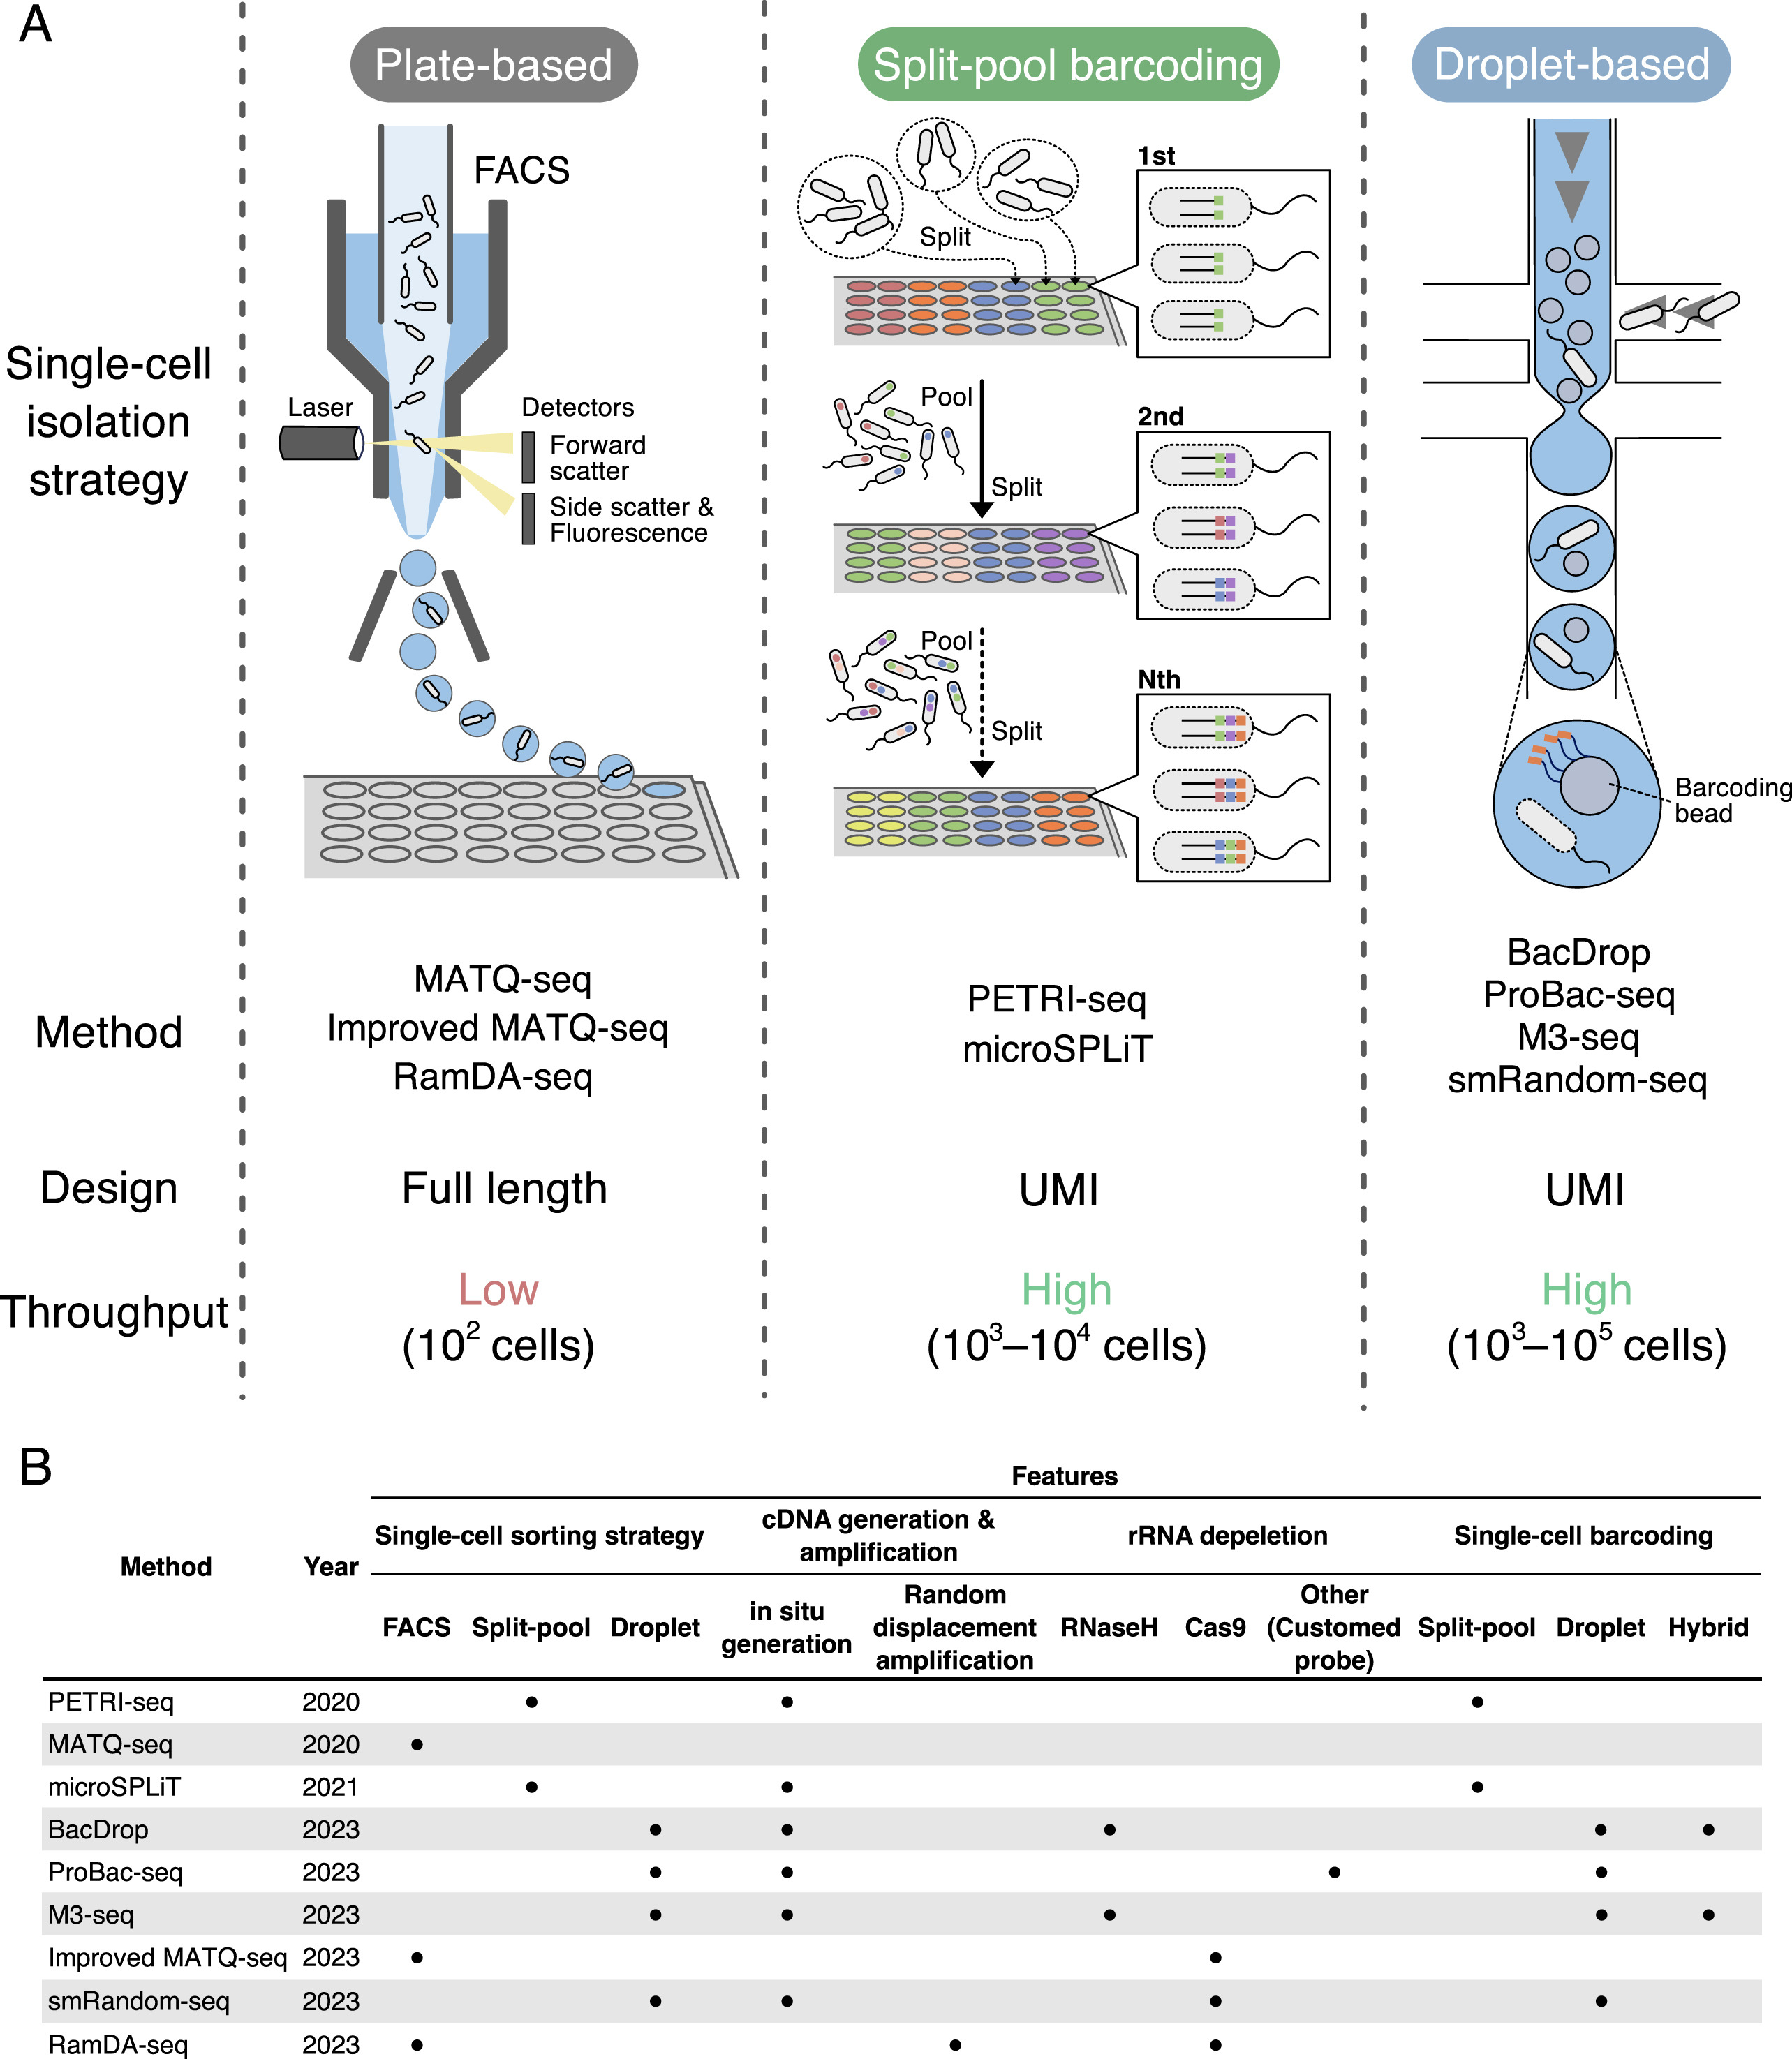
\includegraphics[keepaspectratio]{chapters/../figures/nishimura_review.jpg}}

}

\caption{\label{fig-nishimura_review}Overview of bacterial single-cell
RNA sequencing approaches. (A) Schematic summary of single-cell
isolation strategies employed in bacterial single-cell RNA-seq,
highlighting the key features and distinctions of each approach. FACS,
fluorescent activated cell sorting; UMI, unique molecular identifier.
(B) Summary of features of each bacterial single-cell RNA-seq method,
including MATQ-seq, RamDA-seq, PETRI-seq, microSPLiT, BacDrop,
ProBac-seq, M3-seq, and
smRandom-seq\textsuperscript{\citeproc{ref-nishimura2025}{26}}}

\end{figure}%

\section{MicroSPLiT sequencing library
preparation}\label{microsplit-sequencing-library-preparation}

\begin{figure}

\centering{

\pandocbounded{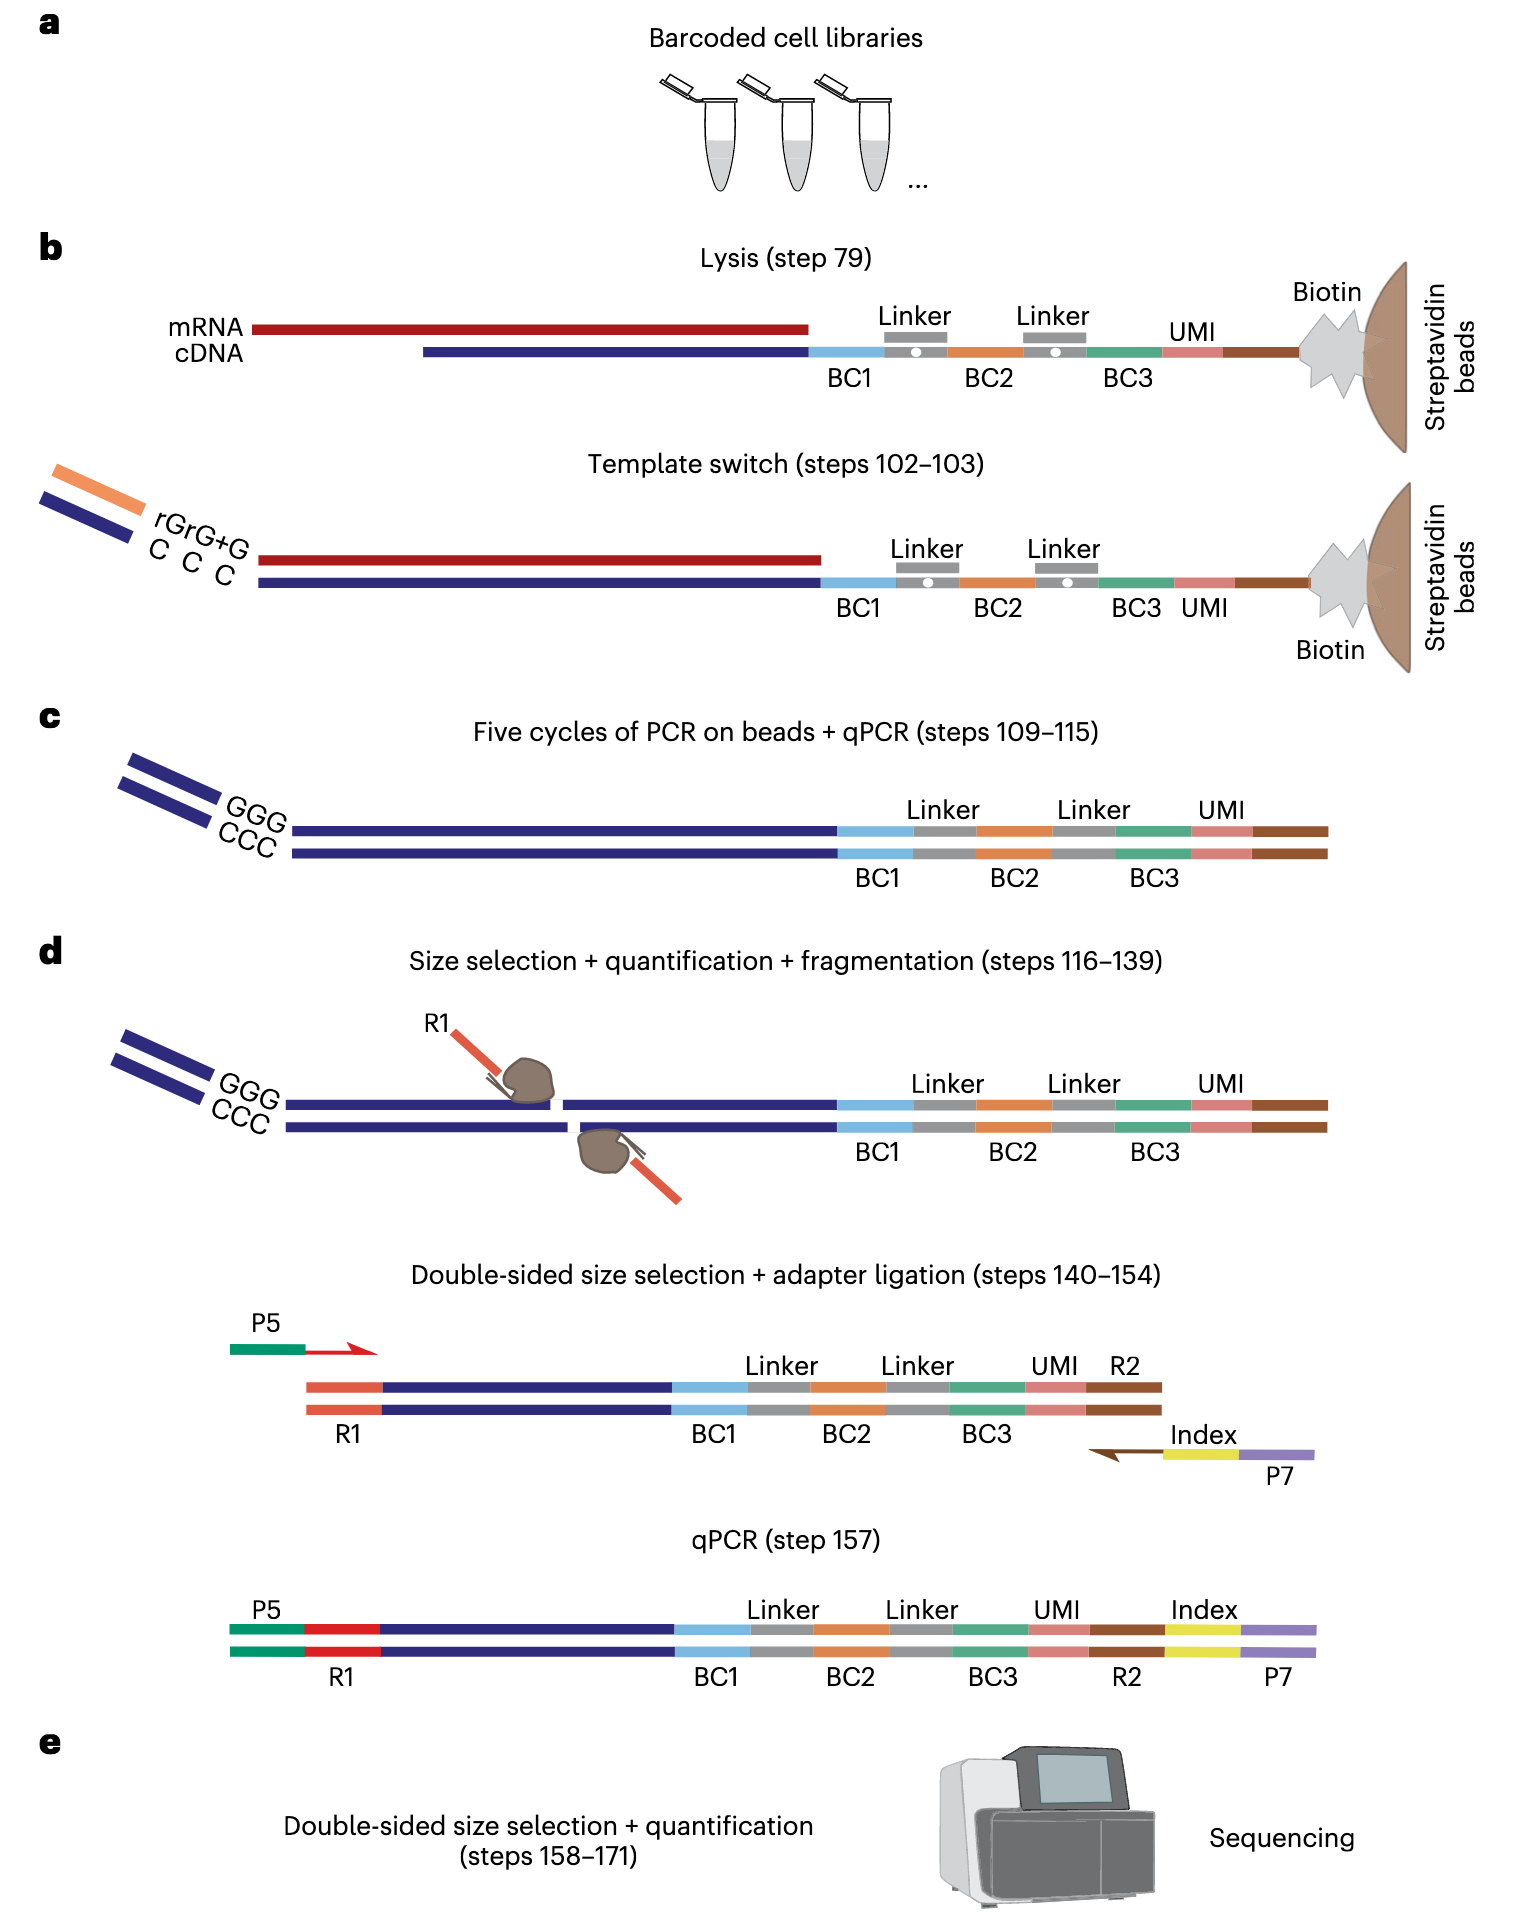
\includegraphics[keepaspectratio]{chapters/../figures/protocol_p2.png}}

}

\caption{\label{fig-protocol-p2}MicroSPLiT sequencing library
preparation. a, Selected sub-libraries with barcoded cells are lysed.
Because cDNA molecules primed with both random hexamer and poly-dT
primers undergo the same downstream reactions, only one of them is shown
for clarity. b, After lysis, cDNA is purified via streptavidin beads.
The cells then undergo an additional RT and template switching step. The
template switch primer has two RNA G bases and a locked nucleic acid G
base (`rGrG+G') sequence to facilitate the binding. c, cDNA is
amplified, and size is selected to eliminate the unwanted short product
(`dimer') from the cDNA amplification product. At this point, the size
and concentration of the cDNA product are quantified (Part 2, Step 127).
d, The library then undergoes fragmentation and adapter ligation. The
desired sequencing product containing the barcodes is amplified with the
primers for both the third barcode adapter and the ligation adapter,
which contain Read 1 (R1) and Read 2 (R2) sequences. Illumina P5 and P7
sequence adapters and a final sub-library index are also appended at
this final PCR step . e, A 0.5--0.7× double size selection then selects
out unwanted fragments. The final product's concentration and size are
measured before sequencing .}

\end{figure}%

\section{TSO removal statistics}\label{sec-appendix-tso}

The following table summarizes the number of R1 reads before and after
TSO removal for each sample, as well as the corresponding percentage.

\begin{longtable}[]{@{}llll@{}}
\caption{TSO removal statistics for each sample. The table shows the
total number of R1 reads, the number of R1 reads after TSO sequence
removal, and the corresponding
percentage.}\label{tbl-tso-removal}\tabularnewline
\toprule\noalign{}
Sample & Total R1 & R1 with TSO removed & Percentage (\%) \\
\midrule\noalign{}
\endfirsthead
\toprule\noalign{}
Sample & Total R1 & R1 with TSO removed & Percentage (\%) \\
\midrule\noalign{}
\endhead
\bottomrule\noalign{}
\endlastfoot
BC\_0076 & 631,393,326 & 153,472,373 & 24.3 \\
BC\_0077 & 325,495,590 & 90,142,002 & 27.7 \\
BC\_0079 & 379,108,253 & 102,386,519 & 27.0 \\
BC\_0080 & 397,654,767 & 99,430,515 & 25.0 \\
\end{longtable}

// Table added to summarize TSO removal efficiency for each sample. //
\ldots{} existing code \ldots{}

\section{Trimming pipeline steps}\label{sec-appendix-trimming-steps}

The following steps were performed sequentially for read trimming, as
implemented in the custom pipeline (see process\_sample.sh). Each step
is performed in paired-end mode to maintain synchronization between R1
and R2 files.

\begin{enumerate}
\def\labelenumi{\arabic{enumi}.}
\item
  \textbf{TSO trimming (Cutadapt):}\\
  Removal of template-switching oligo (TSO) sequences from R1 using
  Cutadapt. This step targets TSO sequences at the 5' end of cDNA reads
  to eliminate technical artifacts.

\begin{Shaded}
\begin{Highlighting}[]
\ExtensionTok{cutadapt} \AttributeTok{{-}j} \VariableTok{$\{SLURM\_CPUS\_PER\_TASK\}} \DataTypeTok{\textbackslash{}}
    \AttributeTok{{-}g} \StringTok{"AAGCAGTGGTATCAACGCAGAGTGAATGGG; min\_overlap=6; max\_errors=0.2"} \DataTypeTok{\textbackslash{}}
    \AttributeTok{{-}g} \StringTok{"CAGAGTGAATGGG; min\_overlap=6; max\_errors=0.2"} \DataTypeTok{\textbackslash{}}
    \AttributeTok{{-}{-}pair{-}filter}\OperatorTok{=}\NormalTok{both }\DataTypeTok{\textbackslash{}}
    \AttributeTok{{-}m}\NormalTok{ 20: }\DataTypeTok{\textbackslash{}}
    \AttributeTok{{-}{-}too{-}short{-}output} \StringTok{"}\VariableTok{$\{output\_dir\}}\StringTok{/}\VariableTok{$\{sample\_name\}}\StringTok{\_R1\_too\_short.fastq.gz"} \DataTypeTok{\textbackslash{}}
    \AttributeTok{{-}{-}too{-}short{-}paired{-}output} \StringTok{"}\VariableTok{$\{output\_dir\}}\StringTok{/}\VariableTok{$\{sample\_name\}}\StringTok{\_R2\_too\_short.fastq.gz"} \DataTypeTok{\textbackslash{}}
    \AttributeTok{{-}o} \StringTok{"}\VariableTok{$\{r1\_output\}}\StringTok{"} \DataTypeTok{\textbackslash{}}
    \AttributeTok{{-}p} \StringTok{"}\VariableTok{$\{r2\_output\}}\StringTok{"} \DataTypeTok{\textbackslash{}}
    \StringTok{"}\VariableTok{$\{r1\_input\}}\StringTok{"} \StringTok{"}\VariableTok{$\{r2\_input\}}\StringTok{"} \DataTypeTok{\textbackslash{}}
    \AttributeTok{{-}{-}report}\OperatorTok{=}\NormalTok{full }\DataTypeTok{\textbackslash{}}
    \AttributeTok{{-}{-}json} \StringTok{"}\VariableTok{$\{output\_dir\}}\StringTok{/}\VariableTok{$\{sample\_name\}}\StringTok{\_stats.json"}
\end{Highlighting}
\end{Shaded}
\item
  \textbf{Initial quality and adapter trimming (Fastp):}\\
  Removal of low-quality bases, polyG/polyX tails, and adapter sequences
  using Fastp. This step also removes the TruSeq Read 2 adapter and I7
  adapter at the end of R1 if present.

\begin{Shaded}
\begin{Highlighting}[]
\ExtensionTok{fastp} \DataTypeTok{\textbackslash{}}
    \AttributeTok{{-}i} \StringTok{"}\VariableTok{$\{r1\_input\}}\StringTok{"} \DataTypeTok{\textbackslash{}}
    \AttributeTok{{-}I} \StringTok{"}\VariableTok{$\{r2\_input\}}\StringTok{"} \DataTypeTok{\textbackslash{}}
    \AttributeTok{{-}o} \StringTok{"}\VariableTok{$\{r1\_output\}}\StringTok{"} \DataTypeTok{\textbackslash{}}
    \AttributeTok{{-}O} \StringTok{"}\VariableTok{$\{r2\_output\}}\StringTok{"} \DataTypeTok{\textbackslash{}}
    \AttributeTok{{-}{-}html} \StringTok{"}\VariableTok{$\{output\_dir\}}\StringTok{/}\VariableTok{$\{sample\_name\}}\StringTok{\_report.html"} \DataTypeTok{\textbackslash{}}
    \AttributeTok{{-}{-}json} \StringTok{"}\VariableTok{$\{output\_dir\}}\StringTok{/}\VariableTok{$\{sample\_name\}}\StringTok{\_report.json"} \DataTypeTok{\textbackslash{}}
    \AttributeTok{{-}{-}report\_title} \StringTok{"microSplit Initial Fastp Report {-} }\VariableTok{$\{sample\_name\}}\StringTok{"} \DataTypeTok{\textbackslash{}}
    \AttributeTok{{-}{-}compression}\NormalTok{ 4 }\DataTypeTok{\textbackslash{}}
    \AttributeTok{{-}{-}verbose} \DataTypeTok{\textbackslash{}}
    \AttributeTok{{-}{-}unpaired1} \StringTok{"}\VariableTok{$\{unpaired1\}}\StringTok{"} \DataTypeTok{\textbackslash{}}
    \AttributeTok{{-}{-}unpaired2} \StringTok{"}\VariableTok{$\{unpaired2\}}\StringTok{"} \DataTypeTok{\textbackslash{}}
    \AttributeTok{{-}{-}length\_required}\NormalTok{ 91 }\DataTypeTok{\textbackslash{}}
    \AttributeTok{{-}{-}dont\_overwrite} \DataTypeTok{\textbackslash{}}
    \AttributeTok{{-}{-}trim\_front1}\NormalTok{ 0 }\DataTypeTok{\textbackslash{}}
    \AttributeTok{{-}{-}trim\_front2}\NormalTok{ 0 }\DataTypeTok{\textbackslash{}}
    \AttributeTok{{-}{-}trim\_tail1}\NormalTok{ 0 }\DataTypeTok{\textbackslash{}}
    \AttributeTok{{-}{-}trim\_tail2}\NormalTok{ 0 }\DataTypeTok{\textbackslash{}}
    \AttributeTok{{-}{-}trim\_poly\_g} \DataTypeTok{\textbackslash{}}
    \AttributeTok{{-}{-}poly\_g\_min\_len}\NormalTok{ 10 }\DataTypeTok{\textbackslash{}}
    \AttributeTok{{-}{-}trim\_poly\_x} \DataTypeTok{\textbackslash{}}
    \AttributeTok{{-}{-}poly\_x\_min\_len}\NormalTok{ 12 }\DataTypeTok{\textbackslash{}}
    \AttributeTok{{-}{-}detect\_adapter\_for\_pe} \DataTypeTok{\textbackslash{}}
    \AttributeTok{{-}{-}adapter\_sequence}\OperatorTok{=}\NormalTok{ATCTCGTATGCCGTCTTCTGCTTGA }\DataTypeTok{\textbackslash{}}
    \AttributeTok{{-}{-}adapter\_sequence}\OperatorTok{=}\NormalTok{AGATCGGAAGAGCACACGTCTGAACTCCAGTCAC}
\end{Highlighting}
\end{Shaded}
\item
  \textbf{PolyA trimming (Cutadapt):}\\
  Removal of polyA stretches (\textgreater=12 nt) and all downstream
  sequences from R1 using Cutadapt, targeting polyA sequences introduced
  during library preparation. This step cleans reads with short cDNA
  that extend into the R2 complementary region, using polyA as a repeat
  sequence (read\_polyA from the library).

\begin{Shaded}
\begin{Highlighting}[]
\ExtensionTok{cutadapt} \AttributeTok{{-}j} \VariableTok{$\{SLURM\_CPUS\_PER\_TASK\}} \DataTypeTok{\textbackslash{}}
    \AttributeTok{{-}a} \StringTok{"A\{12\}; min\_overlap=12; max\_errors=0.2"} \DataTypeTok{\textbackslash{}}
    \AttributeTok{{-}{-}pair{-}filter}\OperatorTok{=}\NormalTok{both }\DataTypeTok{\textbackslash{}}
    \AttributeTok{{-}m}\NormalTok{ 20: }\DataTypeTok{\textbackslash{}}
    \AttributeTok{{-}{-}too{-}short{-}output} \StringTok{"}\VariableTok{$\{output\_dir\}}\StringTok{/}\VariableTok{$\{sample\_name\}}\StringTok{\_R1\_too\_short.fastq.gz"} \DataTypeTok{\textbackslash{}}
    \AttributeTok{{-}{-}too{-}short{-}paired{-}output} \StringTok{"}\VariableTok{$\{output\_dir\}}\StringTok{/}\VariableTok{$\{sample\_name\}}\StringTok{\_R2\_too\_short.fastq.gz"} \DataTypeTok{\textbackslash{}}
    \AttributeTok{{-}o} \StringTok{"}\VariableTok{$\{r1\_output\}}\StringTok{"} \DataTypeTok{\textbackslash{}}
    \AttributeTok{{-}p} \StringTok{"}\VariableTok{$\{r2\_output\}}\StringTok{"} \DataTypeTok{\textbackslash{}}
    \StringTok{"}\VariableTok{$\{r1\_input\}}\StringTok{"} \StringTok{"}\VariableTok{$\{r2\_input\}}\StringTok{"} \DataTypeTok{\textbackslash{}}
    \AttributeTok{{-}{-}report}\OperatorTok{=}\NormalTok{full }\DataTypeTok{\textbackslash{}}
    \AttributeTok{{-}{-}json} \StringTok{"}\VariableTok{$\{output\_dir\}}\StringTok{/}\VariableTok{$\{sample\_name\}}\StringTok{\_stats.json"}
\end{Highlighting}
\end{Shaded}

  This step trims polyA15 and longer stretches that may remain after the
  previous steps.
\item
  \textbf{Specific adapter trimming (Cutadapt):}\\
  Removal of the specific adapter sequence CCACAGTCTCAAGCAC from R1
  using Cutadapt (corresponds to the round 2 linker sequence). This step
  uses the round 2 linker barcode as a reference point and eliminates
  everything behind it, particularly useful for cleaning random hexamer
  sequences with short cDNA that extend into R2 complementary sequences.

\begin{Shaded}
\begin{Highlighting}[]
\ExtensionTok{cutadapt} \AttributeTok{{-}j} \VariableTok{$\{SLURM\_CPUS\_PER\_TASK\}} \DataTypeTok{\textbackslash{}}
    \AttributeTok{{-}a} \StringTok{"CCACAGTCTCAAGCAC; min\_overlap=6; max\_errors=0.1"} \DataTypeTok{\textbackslash{}}
    \AttributeTok{{-}{-}pair{-}filter}\OperatorTok{=}\NormalTok{both }\DataTypeTok{\textbackslash{}}
    \AttributeTok{{-}m}\NormalTok{ 20: }\DataTypeTok{\textbackslash{}}
    \AttributeTok{{-}{-}too{-}short{-}output} \StringTok{"}\VariableTok{$\{output\_dir\}}\StringTok{/}\VariableTok{$\{sample\_name\}}\StringTok{\_R1\_too\_short.fastq.gz"} \DataTypeTok{\textbackslash{}}
    \AttributeTok{{-}{-}too{-}short{-}paired{-}output} \StringTok{"}\VariableTok{$\{output\_dir\}}\StringTok{/}\VariableTok{$\{sample\_name\}}\StringTok{\_R2\_too\_short.fastq.gz"} \DataTypeTok{\textbackslash{}}
    \AttributeTok{{-}o} \StringTok{"}\VariableTok{$\{r1\_output\}}\StringTok{"} \DataTypeTok{\textbackslash{}}
    \AttributeTok{{-}p} \StringTok{"}\VariableTok{$\{r2\_output\}}\StringTok{"} \DataTypeTok{\textbackslash{}}
    \StringTok{"}\VariableTok{$\{r1\_input\}}\StringTok{"} \StringTok{"}\VariableTok{$\{r2\_input\}}\StringTok{"} \DataTypeTok{\textbackslash{}}
    \AttributeTok{{-}{-}report}\OperatorTok{=}\NormalTok{full }\DataTypeTok{\textbackslash{}}
    \AttributeTok{{-}{-}json} \StringTok{"}\VariableTok{$\{output\_dir\}}\StringTok{/}\VariableTok{$\{sample\_name\}}\StringTok{\_stats.json"}
\end{Highlighting}
\end{Shaded}
\item
  \textbf{Linker and additional adapter trimming (Cutadapt):}\\
  Removal of linker and additional adapter sequences from R1 using
  Cutadapt, to further clean the reads. This includes TruSeq Read 2
  adapter (AGATCGGAAGAGCACACGTCTGAACTCCAGTCA), Round 3 linker
  (AGTCGTACGCCGATGCGAAACATCGGCCAC), and Round 2 linker
  (CCACAGTCTCAAGCACGTGGAT).\\
  This step ensures that any remaining linker or adapter sequences are
  removed for certain libraries.

\begin{Shaded}
\begin{Highlighting}[]
\ExtensionTok{cutadapt} \AttributeTok{{-}j} \VariableTok{$\{SLURM\_CPUS\_PER\_TASK\}} \DataTypeTok{\textbackslash{}}
    \AttributeTok{{-}a} \StringTok{"CCACAGTCTCAAGCACGTGGAT; min\_overlap=6; max\_errors=0.2"} \DataTypeTok{\textbackslash{}}
    \AttributeTok{{-}a} \StringTok{"AGTCGTACGCCGATGCGAAACATCGGCCAC; min\_overlap=6; max\_errors=0.2"} \DataTypeTok{\textbackslash{}}
    \AttributeTok{{-}a} \StringTok{"AGATCGGAAGAGCACACGTCTGAACTCCAGTCA; min\_overlap=6; max\_errors=0.2"} \DataTypeTok{\textbackslash{}}
    \AttributeTok{{-}{-}pair{-}filter}\OperatorTok{=}\NormalTok{both }\DataTypeTok{\textbackslash{}}
    \AttributeTok{{-}m}\NormalTok{ 20: }\DataTypeTok{\textbackslash{}}
    \AttributeTok{{-}{-}too{-}short{-}output} \StringTok{"}\VariableTok{$\{output\_dir\}}\StringTok{/}\VariableTok{$\{sample\_name\}}\StringTok{\_R1\_too\_short.fastq.gz"} \DataTypeTok{\textbackslash{}}
    \AttributeTok{{-}{-}too{-}short{-}paired{-}output} \StringTok{"}\VariableTok{$\{output\_dir\}}\StringTok{/}\VariableTok{$\{sample\_name\}}\StringTok{\_R2\_too\_short.fastq.gz"} \DataTypeTok{\textbackslash{}}
    \AttributeTok{{-}o} \StringTok{"}\VariableTok{$\{r1\_output\}}\StringTok{"} \DataTypeTok{\textbackslash{}}
    \AttributeTok{{-}p} \StringTok{"}\VariableTok{$\{r2\_output\}}\StringTok{"} \DataTypeTok{\textbackslash{}}
    \StringTok{"}\VariableTok{$\{r1\_input\}}\StringTok{"} \StringTok{"}\VariableTok{$\{r2\_input\}}\StringTok{"} \DataTypeTok{\textbackslash{}}
    \AttributeTok{{-}{-}report}\OperatorTok{=}\NormalTok{full }\DataTypeTok{\textbackslash{}}
    \AttributeTok{{-}{-}json} \StringTok{"}\VariableTok{$\{output\_dir\}}\StringTok{/}\VariableTok{$\{sample\_name\}}\StringTok{\_stats.json"}
\end{Highlighting}
\end{Shaded}
\item
  \textbf{Final quality and length filtering (Fastp):}\\
  Final trimming with Fastp, including additional adapter removal,
  trimming of fixed bases from the 5' and 3' ends, and filtering for
  minimum read length to ensure high-quality output for downstream
  analysis.\\
  This step trims R1 at both 5' and 3' ends to keep only cDNA and ensure
  clean sequences for downstream analysis.

\begin{Shaded}
\begin{Highlighting}[]
\ExtensionTok{fastp} \DataTypeTok{\textbackslash{}}
    \AttributeTok{{-}i} \StringTok{"}\VariableTok{$\{r1\_input\}}\StringTok{"} \DataTypeTok{\textbackslash{}}
    \AttributeTok{{-}I} \StringTok{"}\VariableTok{$\{r2\_input\}}\StringTok{"} \DataTypeTok{\textbackslash{}}
    \AttributeTok{{-}o} \StringTok{"}\VariableTok{$\{r1\_output\}}\StringTok{"} \DataTypeTok{\textbackslash{}}
    \AttributeTok{{-}O} \StringTok{"}\VariableTok{$\{r2\_output\}}\StringTok{"} \DataTypeTok{\textbackslash{}}
    \AttributeTok{{-}{-}trim\_front1}\NormalTok{ 10 }\DataTypeTok{\textbackslash{}}
    \AttributeTok{{-}{-}trim\_front2}\NormalTok{ 0 }\DataTypeTok{\textbackslash{}}
    \AttributeTok{{-}{-}trim\_tail1}\NormalTok{ 16 }\DataTypeTok{\textbackslash{}}
    \AttributeTok{{-}{-}trim\_tail2}\NormalTok{ 0 }\DataTypeTok{\textbackslash{}}
    \AttributeTok{{-}{-}length\_required}\NormalTok{ 25 }\DataTypeTok{\textbackslash{}}
    \AttributeTok{{-}{-}detect\_adapter\_for\_pe} \DataTypeTok{\textbackslash{}}
    \AttributeTok{{-}{-}adapter\_sequence}\OperatorTok{=}\NormalTok{AAGCAGTGGTATCAACGCAGAGTGAATGGG }\DataTypeTok{\textbackslash{}}
    \AttributeTok{{-}{-}adapter\_sequence}\OperatorTok{=}\NormalTok{CCACAGTCTCAAGCACGTGGAT }\DataTypeTok{\textbackslash{}}
    \AttributeTok{{-}{-}adapter\_sequence}\OperatorTok{=}\NormalTok{AGTCGTACGCCGATGCGAAACATCGGCCAC }\DataTypeTok{\textbackslash{}}
    \AttributeTok{{-}{-}adapter\_sequence}\OperatorTok{=}\NormalTok{AGATCGGAAGAGCACACGTCTGAACTCCAGTCA }\DataTypeTok{\textbackslash{}}
    \AttributeTok{{-}{-}html} \StringTok{"}\VariableTok{$\{output\_dir\}}\StringTok{/}\VariableTok{$\{sample\_name\}}\StringTok{\_report.html"} \DataTypeTok{\textbackslash{}}
    \AttributeTok{{-}{-}json} \StringTok{"}\VariableTok{$\{output\_dir\}}\StringTok{/}\VariableTok{$\{sample\_name\}}\StringTok{\_report.json"} \DataTypeTok{\textbackslash{}}
    \AttributeTok{{-}{-}report\_title} \StringTok{"microSplit Final Fastp Report {-} }\VariableTok{$\{sample\_name\}}\StringTok{"} \DataTypeTok{\textbackslash{}}
    \AttributeTok{{-}{-}compression}\NormalTok{ 4 }\DataTypeTok{\textbackslash{}}
    \AttributeTok{{-}{-}verbose}
\end{Highlighting}
\end{Shaded}
\end{enumerate}

\section{Final effective command line of
STARsolo}\label{sec-appendix-starsolo}

\subsection{STARsolo KneePant filtering
results}\label{sec-appendix-starsolo-kneepant}

As a comparison to our custom filtering approach, we also analyzed the
data using STARsolo's default KneePant filtering method. The following
table presents the results obtained with this alternative filtering
strategy:

Metric \textbar{} KneePant Filtered Data \textbar{}

\begin{table}

\caption{\label{tbl-starsolo-kneepant}STARsolo KneePant filtering
results for comparison}

\begin{minipage}{\linewidth}

\begin{longtable}[]{@{}
  >{\raggedright\arraybackslash}p{(\linewidth - 4\tabcolsep) * \real{0.5244}}
  >{\raggedright\arraybackslash}p{(\linewidth - 4\tabcolsep) * \real{0.1829}}
  >{\raggedright\arraybackslash}p{(\linewidth - 4\tabcolsep) * \real{0.2927}}@{}}
\toprule\noalign{}
\begin{minipage}[b]{\linewidth}\raggedright
-------------------------------------------
\end{minipage} & \begin{minipage}[b]{\linewidth}\raggedright
------------------------
\end{minipage} & \begin{minipage}[b]{\linewidth}\raggedright
\end{minipage} \\
\midrule\noalign{}
\endhead
\bottomrule\noalign{}
\endlastfoot
\textbf{Estimated Number of Cells} & 27,203 & Large population for DoL
analysis \\
\textbf{Mean Reads per Cell} & 470 & Good coverage depth \\
\textbf{Median Reads per Cell} & 381 & Consistent coverage \\
\textbf{Mean UMI per Cell} & 465 & Reliable molecular counting \\
\textbf{Median UMI per Cell} & 378 & Consistent UMI distribution \\
\textbf{Mean Genes per Cell} & 296 & Rich transcriptional profiles \\
\textbf{Median Genes per Cell} & 258 & Consistent gene detection \\
\textbf{Total Genes Detected} & 6,035 & Comprehensive gene coverage \\
\end{longtable}

\end{minipage}%

\end{table}%

\emph{Results obtained using STARsolo's default KneePant filtering
method. This approach would have resulted in approximately 27,000 cells
with higher average coverage per cell, but potentially at the cost of
removing biologically relevant stressed cells that might exhibit lower
quality metrics.}

The KneePant method applies a knee plot analysis to identify the
inflection point in the barcode rank plot, automatically determining the
threshold between genuine cells and background noise. While this method
provides a standardized approach to cell filtering, it may not be
optimal for division of labor analysis where stressed cells with
potentially lower quality metrics could represent important biological
subpopulations.

\subsection{Computing Environment}\label{computing-environment}

The STARsolo analysis was performed on the GenOuest high-performance
computing cluster using the following specifications: - \textbf{Node
type}: bigmem (high-memory node) - \textbf{Memory allocation}: 500GB RAM
- \textbf{CPU threads}: 64 parallel threads

\subsection{STARsolo Command Line}\label{starsolo-command-line}

\begin{Shaded}
\begin{Highlighting}[]
\ExtensionTok{STAR} \DataTypeTok{\textbackslash{}}
\NormalTok{{-}{-}runThreadN 64 }\DataTypeTok{\textbackslash{}}
\NormalTok{{-}{-}genomeDir /path/to/genome\_index }\DataTypeTok{\textbackslash{}}
\NormalTok{{-}{-}readFilesIn }\DataTypeTok{\textbackslash{}}
\NormalTok{/path/to/input/merged\_trimmed{-}R1.fastq.gz }\DataTypeTok{\textbackslash{}}
\NormalTok{/path/to/input/merged\_trimmed{-}R2.fastq.gz }\DataTypeTok{\textbackslash{}}
\NormalTok{{-}{-}readFilesCommand gunzip }\AttributeTok{{-}c} \DataTypeTok{\textbackslash{}}
\NormalTok{{-}{-}outFileNamePrefix /path/to/output/starsolo\_output/ }\DataTypeTok{\textbackslash{}}
\NormalTok{{-}{-}outSAMtype BAM Unsorted }\DataTypeTok{\textbackslash{}}
\NormalTok{{-}{-}outFilterScoreMinOverLread 0 }\DataTypeTok{\textbackslash{}}
\NormalTok{{-}{-}outFilterMatchNmin 50 }\DataTypeTok{\textbackslash{}}
\NormalTok{{-}{-}outFilterMatchNminOverLread 0 }\DataTypeTok{\textbackslash{}}
\NormalTok{{-}{-}alignSJoverhangMin 1000 }\DataTypeTok{\textbackslash{}}
\NormalTok{{-}{-}alignSJDBoverhangMin 1000 }\DataTypeTok{\textbackslash{}}
\NormalTok{{-}{-}soloType CB\_UMI\_Complex }\DataTypeTok{\textbackslash{}}
\NormalTok{{-}{-}soloCBwhitelist }\DataTypeTok{\textbackslash{}}
\NormalTok{/path/to/barcodes/barcode\_round3.txt }\DataTypeTok{\textbackslash{}}
\NormalTok{/path/to/barcodes/barcode\_round2.txt }\DataTypeTok{\textbackslash{}}
\NormalTok{/path/to/barcodes/barcode\_round1.txt }\DataTypeTok{\textbackslash{}}
\NormalTok{{-}{-}soloFeatures Gene GeneFull }\DataTypeTok{\textbackslash{}}
\NormalTok{{-}{-}soloUMIdedup 1MM\_All }\DataTypeTok{\textbackslash{}}
\NormalTok{{-}{-}soloCBmatchWLtype 1MM }\DataTypeTok{\textbackslash{}}
\NormalTok{{-}{-}soloCBposition 0\_10\_0\_17 0\_48\_0\_55 0\_78\_0\_85 }\DataTypeTok{\textbackslash{}}
\NormalTok{{-}{-}soloUMIposition 0\_0\_0\_9 }\DataTypeTok{\textbackslash{}}
\NormalTok{{-}{-}soloMultiMappers Uniform}
\end{Highlighting}
\end{Shaded}

\subsection{STARsolo Parameters
Explanation}\label{starsolo-parameters-explanation}

This section details the key parameters used in our STARsolo analysis
and their significance:

\subsubsection{General STAR Parameters}\label{general-star-parameters}

\begin{itemize}
\tightlist
\item
  \texttt{-\/-runThreadN\ 64} : Use of 64 threads for parallel alignment
\item
  \texttt{-\/-genomeDir} : Path to the reference genome index
\item
  \texttt{-\/-readFilesIn} : Input FASTQ files (R1 and R2)
\item
  \texttt{-\/-readFilesCommand\ gunzip\ -c} : Command to decompress
  FASTQ.gz files
\item
  \texttt{-\/-outFileNamePrefix} : Prefix for output files
\item
  \texttt{-\/-outSAMtype\ BAM\ Unsorted} : Unsorted BAM output format
\end{itemize}

\subsubsection{Filtering Parameters}\label{filtering-parameters}

\begin{itemize}
\tightlist
\item
  \texttt{-\/-outFilterScoreMinOverLread\ 0} : Minimum filtering score
  relative to read length
\item
  \texttt{-\/-outFilterMatchNmin\ 50} : Minimum number of matching bases
  for a valid alignment
\item
  \texttt{-\/-outFilterMatchNminOverLread\ 0} : Minimum match ratio
  relative to read length
\item
  \texttt{-\/-alignSJoverhangMin\ 1000} and
  \texttt{-\/-alignSJDBoverhangMin\ 1000} : Maximum values for splice
  junction detection (set to maximum since bacterial genomes lack
  splicing)
\end{itemize}

\subsubsection{STARsolo-specific
Parameters}\label{starsolo-specific-parameters}

\begin{itemize}
\tightlist
\item
  \texttt{-\/-soloType\ CB\_UMI\_Complex} : Analysis type for cell
  barcodes (CB) and complex UMIs
\item
  \texttt{-\/-soloCBwhitelist} : List of valid cell barcodes for the
  three barcoding rounds
\item
  \texttt{-\/-soloFeatures\ Gene\ GeneFull} : Analysis of features at
  both gene and full transcript levels
\item
  \texttt{-\/-soloUMIdedup\ 1MM\_All} : UMI deduplication with one
  mutation tolerance
\item
  \texttt{-\/-soloCBmatchWLtype\ 1MM} : Cell barcode matching with one
  mutation tolerance
\item
  \texttt{-\/-soloCBposition} : Cell barcode positions in reads (3
  rounds)

  \begin{itemize}
  \tightlist
  \item
    Round 1: 0\_10\_0\_17
  \item
    Round 2: 0\_48\_0\_55
  \item
    Round 3: 0\_78\_0\_85
  \end{itemize}
\item
  \texttt{-\/-soloUMIposition\ 0\_0\_0\_9} : UMI position in reads
\item
  \texttt{-\/-soloMultiMappers\ Uniform} : Uniform distribution of
  multi-mapped reads
\end{itemize}

These parameters were chosen to optimize single-cell detection while
maintaining high alignment quality and accounting for the complexity of
our three-round barcoding protocol.

Each step is performed in paired-end mode to ensure synchronization
between R1 and R2 files. See the pipeline script for implementation
details.

\begin{itemize}
\tightlist
\item
  plan de plaque
\item
  librairies avec TSO
\item
  tableau choix de profondeur / nombre de cellules
\item
  mettre difference entre experience de kuhina et la notre pour les
  resultats de Starsolo
\end{itemize}

\chapter{Annexe B: erferfrefref}\label{annexe-b}

\section{summary stats and features.stats for
Gene}\label{summary-stats-and-features.stats-for-gene}

\begin{verbatim}
                                     nUnmapped      114628761
                                    nNoFeature       20579292
                                 nAmbigFeature      934096737
                         nAmbigFeatureMultimap      934096737
                                      nTooMany              0
                                 nNoExactMatch         124864
                                   nExactMatch     4458742628
                                        nMatch      964094047
                                  nMatchUnique       30022209
                                 nCellBarcodes         689818
                                         nUMIs       29709734
\end{verbatim}

Number of Reads,1284475633 Reads With Valid Barcodes,0.85576 Sequencing
Saturation,0.0104081 Q30 Bases in CB+UMI,0.955089 Q30 Bases in RNA
read,0.957923 Reads Mapped to Genome: Unique+Multiple,0.895694 Reads
Mapped to Genome: Unique,0.0363836 Reads Mapped to Gene: Unique+Multipe
Gene,0.750574 Reads Mapped to Gene: Unique Gene,0.0233731 Estimated
Number of Cells,27268 Unique Reads in Cells Mapped to Gene,11121465
Fraction of Unique Reads in Cells,0.370441 Mean Reads per Cell,407
Median Reads per Cell,331 UMIs in Cells,10998607 Mean UMI per Cell,403
Median UMI per Cell,327 Mean Gene per Cell,253 Median Gene per Cell,221
Total Gene Detected,5894

\section{warning}\label{warning-2}

!!!!! WARNING: while processing
sjdbGTFfile=/projects/microsplit/data/processed\_data/STARsolo\_result/merged\_trimmed/merged/raw\_data/genome\_annotation/genome\_annotation\_PsR401\_fixed.gtf,
line: CP125962.1 Genbank exon 298557 300953 . - 0 transcript\_id
``gene-QLH64\_29550''; gene\_id ``gene-QLH64\_29550''; gene\_name
``QLH64\_29550''; exon end = 300953 is larger than the chromosome
CP125962.1 length = 299955 , will skip this exon

Log of the STARsolo run : Alignment statistics: -----------------------
Number of input reads \textbar{} 1284475633 Average input read length
\textbar{} 135 Uniquely mapped reads number \textbar{} 46733841 Uniquely
mapped reads \% \textbar{} 3.64\% Number of reads mapped to multiple
loci \textbar{} 1103762730 \% of reads mapped to multiple loci
\textbar{} 85.93\% Number of reads unmapped: other \textbar{} 128049614
\% of reads unmapped: other \textbar{} 9.97\% Mismatch rate per base, \%
\textbar{} 0.38\% Fri May 30 15:39:42 CEST 2025 - Pipeline completed!

\subsection{Pretest STARSolo on BC\_0077 without trimming
:}\label{pretest-starsolo-on-bc_0077-without-trimming}

\begin{verbatim}
                                    nNoAdapter              0
                                        nNoUMI              0
                                         nNoCB              0
                                        nNinCB              0
                                       nNinUMI        4467771
                               nUMIhomopolymer        4325324
                                      nTooMany              0
                                      nNoMatch       66837523
                           nMismatchesInMultCB        1680783
                                   nExactMatch      234544811
                                nMismatchOneWL       13639378
                             nMismatchToMultWL              0
\end{verbatim}

barcodes stats

\subsubsection{Genfull summary stats}\label{genfull-summary-stats}

\begin{longtable}[]{@{}ll@{}}
\toprule\noalign{}
Metric & Count \\
\midrule\noalign{}
\endhead
\bottomrule\noalign{}
\endlastfoot
nUnmapped & 89,425,075 \\
nNoFeature & 1,000,851 \\
nAmbigFeature & 152,909,678 \\
nAmbigFeatureMultimap & 152,443,034 \\
nTooMany & 0 \\
nNoExactMatch & 185,805 \\
nExactMatch & 729,180,878 \\
nMatch & 157,719,964 \\
nMatchUnique & 4,847,425 \\
nCellBarcodes & 168,346 \\
nUMIs & 305,287 \\
\end{longtable}

\begin{longtable}[]{@{}ll@{}}
\toprule\noalign{}
Metric & Value \\
\midrule\noalign{}
\endhead
\bottomrule\noalign{}
\endlastfoot
Number of Reads & 325,495,590 \\
Reads With Valid Barcodes & 76.19\% \\
Sequencing Saturation & 93.70\% \\
Q30 Bases in CB+UMI & 92.28\% \\
Q30 Bases in RNA read & 86.19\% \\
Reads Mapped to Genome: Unique+Multiple & 58.16\% \\
Reads Mapped to Genome: Unique & 2.15\% \\
Reads Mapped to GeneFull: Unique+Multiple & 48.46\% \\
Reads Mapped to GeneFull: Unique & 1.49\% \\
Estimated Number of Cells & 66,026 \\
Unique Reads in Cells Mapped to GeneFull & 3,538,648 \\
Fraction of Unique Reads in Cells & 73.00\% \\
Mean Reads per Cell & 53 \\
Median Reads per Cell & 36 \\
UMIs in Cells & 202,967 \\
Mean UMI per Cell & 3 \\
Median UMI per Cell & 2 \\
Mean GeneFull per Cell & 2 \\
Median GeneFull per Cell & 2 \\
Total GeneFull Detected & 5,295 \\
\end{longtable}

\subsubsection{Gene summary stats}\label{gene-summary-stats}

\begin{verbatim}
                                     nUnmapped       89425075
                                    nNoFeature        7350074
                                 nAmbigFeature      147588031
                         nAmbigFeatureMultimap      147588029
                                      nTooMany              0
                                 nNoExactMatch         182600
                                   nExactMatch      704353731
                                        nMatch      151371640
                                  nMatchUnique        3820029
                                 nCellBarcodes         135433
                                         nUMIs         224743
\end{verbatim}

248001599.933

Number of Reads,325495590 Reads With Valid Barcodes,0.76192 Sequencing
Saturation,0.941167 Q30 Bases in CB+UMI,0.922758 Q30 Bases in RNA
read,0.861863 Reads Mapped to Genome: Unique+Multiple,0.581583 Reads
Mapped to Genome: Unique,0.0215405 Reads Mapped to Gene: Unique+Multipe
Gene,0.46505 Reads Mapped to Gene: Unique Gene,0.011736 Estimated Number
of Cells,47264 Unique Reads in Cells Mapped to Gene,2582244 Fraction of
Unique Reads in Cells,0.675975 Mean Reads per Cell,54 Median Reads per
Cell,40 UMIs in Cells,136574 Mean UMI per Cell,2 Median UMI per Cell,2
Mean Gene per Cell,2 Median Gene per Cell,2 Total Gene Detected,4838

\chapter{Annexe C: codcefe}\label{annexe-c}

R2 before trimming

\begin{table}

\caption{\label{tbl-example}R1 before trimming}

\begin{minipage}{\linewidth}

\begin{longtable}[]{@{}llll@{}}
\toprule\noalign{}
Sample Name & Dups & GC & Median len \\
\midrule\noalign{}
\endhead
\bottomrule\noalign{}
\endlastfoot
BC\_0076\_R2 & 88.9\% & 54.0\% & 91bp \\
BC\_0077\_R2 & 18.6\% & 53.0\% & 91bp \\
BC\_0079\_R2 & 20.3\% & 54.0\% & 91bp \\
BC\_0080\_R2 & 88.1\% & 54.0\% & 91bp \\
\end{longtable}

\end{minipage}%

\end{table}%

R2 after trimming

\begin{table}

\caption{\label{tbl-example}R1 after trimming}

\begin{minipage}{\linewidth}

\begin{longtable}[]{@{}llll@{}}
\toprule\noalign{}
Sample Name & Dups & GC & Median len \\
\midrule\noalign{}
\endhead
\bottomrule\noalign{}
\endlastfoot
BC\_0080\_R2 & 92.0\% & 53.0\% & 90bp \\
BC\_0079\_R2 & 23.5\% & 53.0\% & 90bp \\
BC\_0077\_R2 & 21.4\% & 53.0\% & 90bp \\
BC\_0076\_R2 & 92.9\% & 53.0\% & 90bp \\
\end{longtable}

\end{minipage}%

\end{table}%

\begin{table}

\caption{\label{tbl-example}Before trimming}

\begin{minipage}{\linewidth}

\begin{longtable}[]{@{}llll@{}}
\toprule\noalign{}
Sample Name & Dups & GC & Median len \\
\midrule\noalign{}
\endhead
\bottomrule\noalign{}
\endlastfoot
BC\_0076\_R1 & 94.5\% & 55.0\% & 241bp \\
BC\_0077\_R1 & 94.1\% & 53.0\% & 241bp \\
BC\_0079\_R1 & 93.8\% & 53.0\% & 241bp \\
BC\_0080\_R1 & 94.6\% & 54.0\% & 241bp \\
\end{longtable}

\end{minipage}%

\end{table}%

\begin{table}

\caption{\label{tbl-example}After trimming}

\begin{minipage}{\linewidth}

\begin{longtable}[]{@{}llll@{}}
\toprule\noalign{}
Sample Name & Dups & GC & Median len \\
\midrule\noalign{}
\endhead
\bottomrule\noalign{}
\endlastfoot
BC\_0076\_R1 & 98.7\% & 51.0\% & 127bp \\
BC\_0077\_R1 & 98.6\% & 51.0\% & 157bp \\
BC\_0079\_R1 & 98.6\% & 51.0\% & 152bp \\
BC\_0080\_R1 & 98.7\% & 51.0\% & 132bp \\
\end{longtable}

\end{minipage}%

\end{table}%

\clearpage
\thispagestyle{empty}
\vspace*{\fill}
\vspace*{\fill}
\clearpage



% Back cover content
\newpage  % Force a new page
\thispagestyle{empty}  % Page without header or footer
\begin{center}
  {\Huge \textbf{Master's Thesis in Bioinformatics}} \\[2cm]
  {\Large \textbf{University of Rennes}} \\[1cm]
  
\includegraphics[width=0.4\textwidth]{figures/rapport/logo_Univ_Rennes.png} \\[1cm]
  
\includegraphics[width=0.6\textwidth]{figures/rapport/couverture.png} \\[1cm]
  \begin{minipage}{0.8\textwidth}
    \centering
    \textit{This thesis was conducted in the framework of the Master's program in Bioinformatics at the University of Rennes. The research presented here contributes to the field of computational biology and bioinformatics.}
  \end{minipage} \\[1cm]
  \begin{minipage}{0.8\textwidth}
    \centering
    \small
    \textit{© Valentin Goupille - ?meta:year \\ All rights reserved}
  \end{minipage}
\end{center} 


\end{document}
